% !TEX program = pdflatex
% !TEX encoding = UTF-8 Unicode

% Plantilla de la clase `scrbook` del paquete KOMA-script para la
% elaboración de un TFG siguiendo las directrices del la comisión del
% Grado en Matemáticas de la Universidad de Granada.

% Francisco Torralbo Torralbo
% miércoles, 29 de abril de 2020

\documentclass{scrbook}

\KOMAoptions{%
  fontsize=10pt,        % Tamaño de fuente
  paper=a4,             % Tamaño del papel
  headings=normal,      % Tamaño de letra para los títulos: small, normal, big
  % parskip=half,         % Espacio entre párrafos: full (una línea) o half (media línea)
  headsepline=false,    % Una linea separa la cabecera del texto
  cleardoublepage=empty,% No imprime cabecera ni pie en páginas en blanco 
  chapterprefix=false,  % No antepone el texto "capítulo" antes del número
  appendixprefix=false,	% No antepone el texto "Apéndice" antes de la letra
  listof=totoc,		    	% Añade a la tabla de contenidos la lista de tablas y figuras
  index=totoc,			    % Añade a la talba de contenidos una entrada para el índice
  bibliography=totoc,	  % Añade a la tabla de contenidos una entrada para bibliografía
  BCOR=5mm,           % Reserva margen interior para la encuadernación. 
                        % El valor dependerá el tipo de encuadernado y del grosor del libro.
  DIV=10,             % Cálcula el diseño de página según ciertos 
                        % parámetros. Al aumentar el número aumentamos el ancho de texto y disminuimos el ancho del margen. Una opción de 14 producirá márgenes estrechos y texto ancho.
}

% INFORMACIÓN PARA LA VERSIÓN IMPRESA
% Si el documento ha de ser impreso en papel de tamaño a4 pero el tamaño del documento (elegido en \KOMAoptions con la ocpión paper) no es a4 descomentar la línea que carga el paquete `crop` más abajo. El paquete crop se encargará de centrar el documento en un a4 e imprimir unas guías de corte. El procedimiento completo para imprenta sería el siguiente:
% 0. Determinar, según el tipo de encuadernación del documento, el ancho reservado para el proceso de encuadernación (preguntar en la imprenta), es decir, la anchura del área del papel que se pierde durante el proceso de encuadernación. Fijar la varibale BCOR de \KOMAoptions a dicho valor.
% 1. Descomentar la siguiente línea e imprimir una única página con las guías de corte
% 2. Cambiar la opción `cross` por `cam` (o `off`) en el paquete crop y volver a compilar. Imprimir el documento (las guías de corte impresas no inferfieren con el texto).
% 3. Usar la página con las guías impresas en el punto 1 para cortar todas las páginas.

% \usepackage[a4, odd, center, pdflatex, cross]{crop} % Permite imprimir el documento en un a4 (si el tamaño es más pequeño) mostrando unas guías de corte. Útil para imprenta.

% VERSIÓN ELECTRÓNICA PARA TABLETA
% Las opciones siguientes seleccionan un tamaño de impresión similar a una tableta de 9 pulgadas con márgenes estrechos. Útil para producir una versión en pdf para ser leída en una tableta en lugar de impresa.
% Para que la portada quede centrada correctamente hay que editar el
% archivo `portada.tex` y eliminar el entorno `addmargin`

% \KOMAoptions{fontsize=10pt, paper=19.7104cm:14.7828cm, twoside=false, BCOR=0cm, DIV=14}

% ---------------------------------------------------------------------
%	PAQUETES 
% ---------------------------------------------------------------------

% CODIFICACIÓN E IDIOMA
% ---------------------------------------------------------------------
\usepackage[utf8]{inputenc} 			    % Codificación de caracteres

% Selección del idioma: cargamos por defecto inglés y español (aunque este último es el idioma por defecto para el documento). Cuando queramos cambiar de idioma escribiremos:
% \selectlanguage{english} o \selectlanguage{spanish}

\usepackage[english, spanish, es-nodecimaldot, es-noindentfirst, es-tabla]{babel}

% Opciones cargadas para el paquete babel:
  % es-nodecimaldot: No cambia el punto decimal por una coma en modo matemático.
  % es-noindentfirst: No sangra los párrafos tras los títulos.
  % es-tabla: cambia el título del entorno `table` de "Cuadro" a "Tabla"

% Otras opciones del paquete spanish-babel:
  \unaccentedoperators % Desactiva los acentos en los operadores matemáticso (p.e. \lim, \max, ...). Eliminar esta opción si queremos que vayan acentuados

% MATEMÁTICAS
% ---------------------------------------------------------------------
\usepackage{amsmath, amsthm, amssymb} % Paquetes matemáticas
\usepackage{mathtools}                % Añade mejoras a amsmath
\mathtoolsset{showonlyrefs=true}      % sólo se numeran las ecuaciones que se usan
\usepackage[mathscr]{eucal} 					% Proporciona el comando \mathscr para
                                      % fuentes de tipo manuscrito en modo matemático sin sobreescribir el comando \mathcal
\usepackage{cancel}
\usepackage{graphbox,graphicx}
\usepackage[ruled]{algorithm2e}
% \usepackage{algpseudocode}
% \usepackage{algorithm}


% TIPOGRAFÍA 
% ---------------------------------------------------------------------
% El paquete microtype mejora la tipografía del documento.
\usepackage[activate={true,nocompatibility},final,tracking=true,kerning=true,spacing=true,factor=1100,stretch=10,shrink=10]{microtype}

% Las tipografías elegidas para el documento, siguiendo la guía de estilo de la UGR,
% son las siguientes
% Normal font: 			URW Palladio typeface. 
% Sans-serif font: 	Gill Sans
% Monospace font: 	Inconsolata
\usepackage[T1]{fontenc}
\usepackage[sc, osf]{mathpazo} \linespread{1.05}         
\usepackage[scaled=.95,type1]{cabin} % sans serif in style of Gill Sans
% Si el paquete cabin da error usar el siguiente comando en su lugar
% \renewcommand{\sfdefault}{iwona} 
\usepackage{inconsolata}

% Selecciona el tipo de fuente para los títulos (capítulo, sección, subsección) del documento.
\setkomafont{disposition}{\sffamily\bfseries}

% Cambia el ancho de la cita. Al inicio de un capítulo podemos usar el comando \dictum[autor]{cita} para añadir una cita famosa de un autor.
\renewcommand{\dictumwidth}{0.45\textwidth} 

\recalctypearea % Necesario tras definir la tipografía a usar.

\usepackage{setspace}
% TABLAS, GRÁFICOS Y LISTADOS DE CÓDIGO
% ---------------------------------------------------------------------
\usepackage{booktabs}
% \renewcommand{\arraystretch}{1.5} % Aumenta el espacio vertical entre las filas de un entorno tabular

\usepackage{lipsum}
\usepackage{listings}
\usepackage{jslistings}
\input{listings-glsl.prf}
% \usepackage[outputdir=../]{minted}

\usepackage{color}
\usepackage{nicefrac}
\usepackage{minted}

\definecolor{dkgreen}{rgb}{0,0.6,0}
\definecolor{gray}{rgb}{0.5,0.5,0.5}
\definecolor{mauve}{rgb}{0.58,0,0.82}

\lstset{frame=tb,
  language=[11]C++,
  aboveskip=3mm,
  belowskip=3mm,
  showstringspaces=false,
  columns=flexible,
  basicstyle={\small\ttfamily},
  numbers=none,
  numberstyle=\tiny\color{gray},
  keywordstyle=\color{blue},
  commentstyle=\color{dkgreen},
  stringstyle=\color{mauve},
  breaklines=true,
  breakatwhitespace=true,
  tabsize=3
  frame = single
}

\usepackage{textcmds}   % para poder poner ""
\usepackage{xcolor, graphicx}
% Carpeta donde buscar los archivos de imagen por defecto
\graphicspath{{img/}}

% IMAGEN DE LA PORTADA
% Existen varias opciones para la imagen de fondo de la portada del TFG. Todas ellas tienen en logotipo de la universidad de Granada en la cabecera. Las opciones son las siguientes:
% 1. portada-ugr y portada-ugr-color: diseño con marca de agua basada en el logo de la UGR (en escala de grises y color).
% 2. portada-ugr-sencilla y portada-ugr-sencilla-color: portada únicamente con el logotipo de la UGR en la cabecera.
\usepackage{eso-pic}
\newcommand\BackgroundPic{%
	\put(0,0){%
		\parbox[b][\paperheight]{\paperwidth}{%
			\vfill
			\centering
      % Indicar la imagen de fondo en el siguiente comando
			
\includegraphics[width=\paperwidth,height=\paperheight,%
			keepaspectratio]{portada-ugr-sencilla}%
			\vfill
}}}

% \usepackage{listings} % Para la inclusión de trozos de código

% CABECERAS
% ---------------------------------------------------------------------
% Si queremos modificar las cabeceras del documento podemos usar el paquete
% `scrlayer-scrpage` de KOMA-Script. Consultar la documentación al respecto.
% \usepackage[automark]{scrlayer-scrpage}

% VARIOS
% ---------------------------------------------------------------------

%\usepackage{showkeys}	% Muestra las etiquetas del documento. Útil para revisar las referencias cruzadas.

% ÍNDICE 
% Para generar el índice hay que compilar el documento con MakeIndex. Generalmente los editores se encargan de ello automáticamente.
% ----------------------------------------------------------------------
% \index{} para añadir un elemento
% \index{main!sub} para añadir un elementos "sub" bajo la categoría "main".
% \index{termino|textbf} para dar formato al número de página (negrita).
% \index{termino|see{termino relacionado}} para crear una referencia cruzada

% Ejemplo: \index{espacio homogéneo}, \index{superficie!mínima}, \index{esfera|see{espacio homogéneo}}

% Activar los siguientes comandos para generar el índice terminológico. Ver también comandos al final de este documento para incluir dicho índice en el pdf final.
% \usepackage{makeidx}
% \makeindex

% Para revisar las entradas al índice conforme las incluimos en el documento es útil el siguiente paquete. Conviene observar que mientras esté cargado no se generará el índice.
%\usepackage{showidx} % Muestra en el margen del documento las entradas añadidas al índice. Útil para revisar el documento. Si está activo el índice no se genera

% ---------------------------------------------------------------------
% COMANDOS Y ENTORNOS
% ---------------------------------------------------------------------
% Cargamos un archivo externo donde hemos incluido todos los comandos
% propios que vamos a usar en el documento.
% DEFINICIÓN DE COMANDOS Y ENTORNOS

% CONJUNTOS DE NÚMEROS

\newcommand{\N}{\mathbb{N}}     % Naturales
\newcommand{\R}{\mathbb{R}}     % Reales
\newcommand{\Z}{\mathbb{Z}}     % Enteros
\newcommand{\Q}{\mathbb{Q}}     % Racionales
\newcommand{\C}{\mathbb{C}}     % Complejos
\newcommand{\Nn}{\mathbb{N}^n}
\newcommand{\Max}{\text{máx}}
\newcommand{\Min}{\text{mín}}
\newcommand{\smin}{\text{smín}}
\newcommand{\smax}{\text{smáx}}
\newcommand{\lex}{\le_{\text{lex}}}
\newcommand{\expf}{\text{exp}(f)}
\newcommand{\lcf}{\text{lc}(f)}
\newcommand{\lc}{\text{lc}}
\newcommand{\sm}{\text{sm}}
\newcommand{\lcg}{\text{lc}(g)}
\newcommand{\lmf}{\text{lm}(f)}
\newcommand{\lm}{\text{lm}}
\newcommand{\ltf}{\text{lt}(f)}
\newcommand{\lt}{\text{lt}}
\newcommand{\rem}{\text{rem}}
\newcommand{\lcm}{\text{lcm}}
\renewcommand{\gcd}{\text{gcd}}
\newcommand{\supp}{\text{supp}}
\newcommand{\sdf}{\text{sdf}}
\newcommand{\reduces}{\stackrel{G}{\to} }
\newcommand*{\mybox}[1]{\framebox{\mystrut #1}}

% TEOREMAS Y ENTORNOS ASOCIADOS

% \newtheorem{theorem}{Theorem}[chapter]
\newtheorem*{teorema*}{Teorema}
\newtheorem{teorema}{Teorema}[chapter]
\newtheorem{proposicion}{Proposición}[chapter]
\newtheorem{lema}{Lema}[chapter]
\newtheorem{corolario}{Corolario}[chapter]

\theoremstyle{definition}
\newtheorem{definicion}{Definición}[chapter]
\newtheorem{ejemplo}{Ejemplo}[chapter]

\theoremstyle{remark}
\newtheorem{observacion}{Observación}[chapter]


% --------------------------------------------------------------------
% INFORMACIÓN DEL TFG Y EL AUTOR
% --------------------------------------------------------------------
\usepackage{xspace} % Para problemas de espaciado al definir comandos

\usepackage{caption}
\usepackage{subcaption}
\newcommand{\miTitulo}{Visualización de Superficies 3D\xspace}
\newcommand{\miNombre}{Daniel Zufrí Quesada\xspace}
\newcommand{\miGrado}{Doble Grado en Ing. Informática y Matemáticas}
\newcommand{\miFacultad}{ETSIIT, Facultad de Ciencias}
\newcommand{\miUniversidad}{Universidad de Granada}
% Añadir tantos tutores como sea necesario separando cada uno de ellos
% mediante el comando `\medskip` y una línea en blanco
\newcommand{\miTutor}{
  Carlos Ureña Almagro \\ \emph{Departamento de Lenguajes y Sistemas Informáticos}
  
  \medskip
  
  Pedro A. García Sánchez \\ \emph{Departamento de Álgebra}
}
\newcommand{\miCurso}{2022-2023\xspace}

% HYPERREFERENCES
% --------------------------------------------------------------------
\usepackage{xurl}
\usepackage{hyperref}
% Opciones para el paquete hyperref
%----------------------------------

\hypersetup{%
    % hidelinks,            % Enlaces sin color ni borde. El borde no se imprime
    linkbordercolor=0.8 0 0,
    citebordercolor=0 0.8 0,
    citebordercolor=0 0.8 0,
    colorlinks = true,            % Color en texto de los enlaces. Comentar esta línea o cambiar `true` por `false` para imprimir el documento.
    linkcolor = [rgb]{0.5, 0, 0}, % Color de los enlaces internos
    urlcolor = [rgb]{0, 0, 0.5},  % Color de los hipervínculos
    citecolor = [rgb]{0, 0.5, 0}, % Color de las referencias bibliográficas
    pdftitle={\miTitulo},%
    pdfauthor={\textcopyright\ \miNombre, \miFacultad, \miUniversidad},%
    pdfsubject={Trabajo de fin de Grado},%
    pdfkeywords={},%
    pdfcreator={pdfLaTeX},%
}

% Redefinición del estilo para mostrar las referencias cruzadas en la bibliografía.
% \renewcommand*{\backref}[1]{}
% \renewcommand{\backrefsep}{, }
% \renewcommand{\backreftwosep}{ y }
% \renewcommand{\backreflastsep}{ y }
% \renewcommand*{\backrefalt}[4]{{\footnotesize [%
%     \ifcase #1 No citado%
%     \or Citado en pág.~#2%
%     \else Citado en págs. #2%
%     \fi%
% ]}}

% Etiquetas en español para el comando \autoref
\def\chapterautorefname{Capítulo}
\def\appendixautorefname{Apéndice}
\def\sectionautorefname{Sección}
\def\subsectionautorefname{Subsección}
\def\figureautorefname{Fig.}
\def\tableautorefname{Tabla}

\def\teoremaautorefname{Teorema}
\def\proposicionautorefname{Proposición}
\def\lemaautorefname{Lema}
\def\corolarioautorefname{Corolario}
\def\definicionautorefname{Def.}
\def\observacionautorefname{Observación}
\def\ejemploautorefname{E.j.}

% Pone automáticamente un parántesis para las ecuaciones
\def\equationautorefname~#1\null{(#1)\null}


\begin{document}

% --------------------------------------------------------------------
% FRONTMATTER
% -------------------------------------------------------------------
\frontmatter % Desactiva la numeración de capítulos y usa numeración romana para las páginas

% \pagestyle{plain} % No imprime cabeceras

% !TeX root = ../libro.tex
% !TeX encoding = utf8

%*******************************************************
% Titlepage
%*******************************************************
\begin{titlepage}
  \AddToShipoutPicture*{\BackgroundPic}
  \phantomsection 
  \pdfbookmark[1]{Título}{title}

  % Para que el título esté centrado en la página.
  % Los valores numéricos deberán elegirse de acuerdo con el diseño de
  % página (sobre todo si se cambia la opción BCOR o DIV).
  \begin{addmargin}[2.575cm]{0cm}
  \begin{flushleft}
    \Large  
    \hfill\vfil

    \large{\textsf{\miFacultad}}
    \vfill

    {\large\textsc\miGrado} \vfill


    {\large\textsc{trabajo de fin de grado}}

    \begin{flushleft}
      \Huge
      \setstretch{0.8}
      \miTitulo

      \bigskip
      \Large
      \setstretch{0.8}
      \miSubtitulo
    \end{flushleft}

    \vfill\vfill\vfill\vfill

    \textsf{\normalsize{Presentado por:}}\\
    {\normalsize\textrm{\miNombre}} 
    \bigskip

    \textsf{\normalsize{Tutores:}}\\
    {\normalsize\rmfamily\miTutor}

    \bigskip
    \textsf{\normalsize{Curso académico \miCurso}}
  \end{flushleft}  
  \end{addmargin}       

\end{titlepage}   
\cleardoublepage
\endinput

%% !TeX root = ../libro.tex
% !TeX encoding = utf8

%*******************************************************
% Little Dirty Titlepage
%*******************************************************

\thispagestyle{empty}

\begin{center}
  \large  

  \vspace*{\stretch{1}}

  \begingroup
  \huge{\miTitulo} \\ \bigskip
  \endgroup

  \textrm{\miNombre}

  \vspace{\stretch{5}}

\end{center}  

\newpage
\thispagestyle{empty}

\hfill

\vfill

\miNombre \textit{\miTitulo}.

Trabajo de fin de Grado. Curso académico \miCurso.
\bigskip

\begin{minipage}[t]{0.25\textwidth}
  \flushleft
  \textbf{Responsable de tutorización}
\end{minipage}
\begin{minipage}[t]{0.45\textwidth}
  \flushleft
  \miTutor
\end{minipage}
\begin{minipage}[t]{0.30\textwidth}
  \flushright
  \miGrado
  \medskip

  \miFacultad
  \medskip

  \miUniversidad
\end{minipage}

\newpage
\endinput

%% !TeX root = ../libro.tex
% !TeX encoding = utf8
%
%*******************************************************
% Declaración de originalidad
%*******************************************************

\thispagestyle{empty}

\hfill\vfill

\textsc{Declaración de originalidad}\\\bigskip

D./Dña. \miNombre \\\medskip

Declaro explícitamente que el trabajo presentado como Trabajo de Fin de Grado (TFG), correspondiente al curso académico \miCurso, es original, entendida esta, en el sentido de que no ha utilizado para la elaboración del trabajo fuentes sin citarlas debidamente.
\medskip

En Granada a \today 
\begin{flushleft} 
Fdo: \miNombre 

\end{flushleft}

\vfill

\cleardoublepage
\endinput

%% !TeX root = ../libro.tex
% !TeX encoding = utf8

%*******************************************************
% Dedication
%*******************************************************
\thispagestyle{empty}
\phantomsection 
\pdfbookmark[1]{Dedicatoria}{Dedicatoria}

\hfill
\vfill

\begin{flushright}
\itshape
Dedicatoria (opcional) \\
Ver archivo \texttt{preliminares/dedicatoria.tex}
\end{flushright}

\vfill

\cleardoublepage
\endinput
                % Opcional
% !TeX root = ../libro.tex
% !TeX encoding = utf8

%*******************************************************
% Table of Contents
%*******************************************************
\phantomsection
\pdfbookmark[0]{\contentsname}{toc}

\setcounter{tocdepth}{2} % <-- 2 includes up to subsections in the ToC
\setcounter{secnumdepth}{3} % <-- 3 numbers up to subsubsections

% \manualmark
% \markboth{\textsc{\contentsname}}{\textsc{\contentsname}}
\tableofcontents 

%*******************************************************
% List of Figures and of the Tables
%*******************************************************

    % *******************************************************
    %  List of Figures
    % *******************************************************    
    \phantomsection 
    % \listoffigures

    %*******************************************************
    % List of Tables
    %*******************************************************
    \phantomsection 
    % \listoftables
    
    %*******************************************************
    % List of Listings
    % The package \usepackage{listings} is needed
    %*******************************************************      
	  % \phantomsection 
    % \renewcommand{\lstlistlistingname}{Listados de código}
    % \lstlistoflistings 

\cleardoublepage

%% !TeX root = ../libro.tex
% !TeX encoding = utf8

%*******************************************************
% Agradecimientos
%*******************************************************

\chapter{Agradecimientos}



\cleardoublepage
\endinput
            % Opcional

% \pagestyle{scrheadings} % A partir de ahora sí imprime cabeceras

% !TeX root = ../libro.tex
% !TeX encoding = utf8
%
%*******************************************************
% Summary
%*******************************************************

\selectlanguage{english}
\chapter{Abstract}

\selectlanguage{spanish} 
\endinput

% !TeX root = ../libro.tex
% !TeX encoding = utf8
%
%*******************************************************
% Introducción
%*******************************************************

% \manualmark
% \markboth{\textsc{Introducción}}{\textsc{Introducción}} 

\chapter{Introducción}\label{cap:intro}
En el campo de los gráficos generados por computador, el método más asentado para describir objetos tridimensionales es mediante mallas de polígonos. Cuando se trata de superficies, la representación implícita es también bastante usada debido a la facilidad que aporta a la hora de realizar geometría de sólidos constructiva o representar objetos sólidos. Sin embargo, esta representación no es apta para ser usada en tiempo real, y es aquí donde en los últimos años ha surgido un enfoque alternativo que muestra un gran potencial: la utilización de funciones distancia con signo (SDF). Estas permiten representar objetos geométricos realmente complejos a través de una única función escalar que asigna a cada punto del espacio su distancia signada respecto a la frontera del objeto  en tiempo real. Esta técnica está cada vez más presente en los programas de modelado y visualización actuales, como explica en el siguiente capítulo, principalmente porque esta representación es especialmente útil para la generación de imágenes y el renderizado en tiempo real, ofreciendo ventajas significativas en términos de eficiencia y precisión respecto otros métodos tradicionales.\newline

El propósito principal de este Trabajo de Fin de Grado es la creación de una aplicación web interactiva que facilite la creación e interacción con superficies generadas a través de SDFs usando una estructura en forma de árbol de forma intuitiva para el usuario sin que este necesite conocimientos al respecto. No obstante, dado que en el ámbito matemático la representación de superficies suele ser a través de ecuaciones implícitas o paramétricas, estudiaremos también como obtener una SDF que represente la misma información que estas ecuaciones, siendo de especial interés este último caso. Para lograr este objetivo, llevaremos a cabo el desarrollo de la aplicación aprovechando las tecnologías web y \textit{frameworks} modernos así como desarrollando nuestras propias herramientas, evaluando la eficiencia y el rendimiento de la aplicación en términos de tiempos de respuesta y calidad visual. Así, los objetivos que nos proponemos alcanzar con nuestra aplicación son los siguientes.\newline
\begin{itemize}
    \item Comprensión profunda de las \textbf{funciones distancia con signo}, sus propiedades y aplicaciones tanto en el ámbito matemático como en el de la Informática Gráfica (IG).
    \item Análisis de la teoría de polinomios en varias variables y soluciones al problema de implicitación, principalmente usando \textbf{bases de Gröbner} y enfocando su uso al \textbf{problema de implicitación} para obtener la SDF asociada a una superficie paramétrica.
    \item Desarrollo de una aplicación web para la representación y manipulación de SDFs a través de un modelo de operaciones con estructura de árbol.
\end{itemize}

El código fuente de la aplicación y su \textit{build} para ejecución local se encuentra disponible en el repositorio \href{https://github.com/Daniel2000815/SDF-Visualizer/}{https://github.com/Daniel2000815/SDF-Visualizer/}. También se puede ejecutar directamente desde el navegador en \href{https://daniel2000815.github.io/SDF-Visualizer/}{https://daniel2000815.github.io/SDF-Visualizer/}.

\section*{Estructura del documento}
Los temas que acabamos de introducir se desarrollan con detalle a lo largo del trabajo como sigue:
\begin{itemize}
    \item En el \autoref{chapter1} exploraremos los fundamentos teóricos y matemáticos de las SDFs que nos servirán de motivación y serán necesarios en el resto de capítulos, estudiando con especial interés su diferenciabilidad (\autoref{sec:dif}). Comprenderemos la capacidad de las SDFs para describir superficies y volúmenes de manera precisa y compacta, así como las posibilidades para su manipulación (\autoref{sec:operaciones}), como las operaciones booleanas o las deformaciones. Acabaremos explicando como podemos obtener un SDF a partir de una ecuación implícita (\autoref{sec:aprox}) y resolviendo el problema de implicitación con bases de Gröbner (\autoref{sec:grobner} y resultantes (\autoref{sec:radical}) para así poder sacar provecho de las ventajas que nos aporta el uso de las SDFs también a superficies definidas mediante ecuaciones implícitas o paramétricas. 
    
    \item En el \autoref{cap:2} analizaremos las diferencias y similitudes de los dos principales métodos de renderizado actuales: la rasterización y el \textit{raytracing}. Veremos paso a paso como combinar ambas técnicas para conseguir representar cualquier superficie dada por una SDF mediante \textit{spheretracing} (\autoref{sec:render}). Para ello empezaremos definiendo la geometría necesaria con un \textit{vertex shader} asociado en la \autoref{sec:lienzo}, habiéndonos familiarizado previamente con los diferentes sistemas de coordenadas comúnmente usados en IG. Posteriormente veremos cómo colorear la geometría definida anteriormente para representar la superficie sobre ella a través de un \textit{fragment shader}. Finalmente, incluiremos el modelo de iluminación de Blinn-Phong (\autoref{sec:ilum}), al cual añadiremos realismo usando algoritmos avanzados de cálculo de sombras (\autoref{sec:sombras}) y oclusión ambiental (\autoref{sec:ao}), y usaremos \textit{antialiasing} para obtener una imagen lo más libre de imperfecciones posible, todo esto usando un \textit{hardware} accesible a todo tipo de usuario.
    
    \item En el \autoref{chapter3} explicaremos el proceso de diseño y desarrollo de la aplicación en React, poniendo especial atención en cómo trasladar la teoría que vimos en la \autoref{sec:render} sobre \textit{spheretracing} a la práctica usando WebGL y GLSL (\autoref{sec:lienzoImplem}) y el funcionamiento interno del editor de nodos en árbol, con el que crear nuevas superficies (\autoref{sec:editorNodos}) a partir de las ya existentes, y nuestra librería de polinomios en varias variables (\autoref{sec:lib}).
    
    \item En el \autoref{chapter4} analizaremos el proceso de validación que se ha seguido a lo largo del desarrollo de la aplicación y la librería, y como estas se comportan en escenarios de estrés, incluyendo pruebas de rendimiento del visualizador basado en SDFs.
    
    \item Finalmente, en el \autoref{chapter5} haremos una reflexión sobre lo que aporta este trabajo al panorama actual, qué objetivos de los propuestos se han alcanzado, y como este puede ser continuado en el futuro.
\end{itemize}

\endinput

\chapter{Estado del arte}


% --------------------------------------------------------------------
% MAINMATTER
% --------------------------------------------------------------------
\mainmatter % activa la numeración de capítulos, resetea la numeración de las páginas y usa números arábigos

% !TeX root = ../libro.tex
% !TeX encoding = utf8
\chapter{Fundamentos matemáticos: las SDFs}
Estamos acostumbrados a representar superficies en $\R^3$ a través de ecuaciones paramétricas e implícitas. En el caso de las paramétricas se asigna a cada tupla de parámetros un punto, mientras que para las implícitas, dado un punto la ecuación indica si este se encuentra dentro o fuera de la superficie. El tipo de superficies implícitas más comúnmente estudiado es el de las superficies algebraicas, variedades algebraicas de dimensión 2. Existen varios métodos para la visualización de este tipo de superficies. Uno de ellos es tratar de generar una malla de polígonos previamente a partir de la ecuación para después ser visualizada en tiempo real usando los métodos clásicos. El problema de este método es que no siempre se puede aplicar y conlleva pérdida de precisión en la representación de la superficie. Otro método es el \textit{raytracing}, pero este también puede llegar a perder precisión, además de que es muy lento, haciendo que la representación de una superficie tan simple como una esfera sea computacionalmente muy costoso.\newline

Como solución a esto, T. Sederberg y A.Zundel \cite{Sederberg1989ScanLD} presentaron en 1989 un método capaz de representar superficies algebraicas sin pérdida de información y de manera eficiente, capaz además de trabajar con siluetas, intersección de curvas y operaciones booleanas. En 1889 John C. Hart \cite{hart2} presenta una técnica de \textit{raymarching} para la representación de fractales usando funciones distancia con signo. Posteriormente, en 1995 \cite{hart} generaliza esta técnica con el uso de \textit{spheretracing} para la representación de cualquier superficie implícita (algebraica o no), punto de partida de este trabajo.\newline

Este método nos permitirá representar cualquier superficie en tiempo real con un coste computacionalmente muy bajo y a cualquier nivel de detalle. No obstante, para usarlo debemos comprender qué son las funciones distancia con signo, sus propiedades, y como trabajar con ellas.

\begin{definicion}\label{def:sdf}
  Sea $\Omega \subset \R^3$. La \textbf{función distancia} asociada a $\Omega$, que llamamos $d_{\Omega}$ es el campo escalar que a cada punto de $\R^3$ le asigna su menor distancia a la frontera de $\Omega$:
    \begin{align*}
          d_{\Omega} \colon \R^3 &\to \R_0^+,\\
          x &\mapsto \inf\{\Vert x-y\Vert) \colon y \in \delta\Omega\}.
    \end{align*}

    Cuando $\Omega$ sea cerrado, podremos usar el mínimo en lugar del ínfimo.
\end{definicion}

\begin{definicion}\label{d:sdf}
  Sea $\Omega \subset \R^3$. La \textbf{función distancia con signo} asociada a $\Omega$ es el campo escalar de la forma:
  \begin{align*}
          \phi_{\Omega} \colon \R^3 &\to \R,\\
          x &\mapsto \begin{cases}
      d_{\Omega}(x),  &x\in \R^3\setminus \mathring{\Omega}, \\
      -d_{\Omega}(x), &x\in \mathring{\Omega}.
    \end{cases}
    \end{align*}

  En general, nos referiremos a esta función por sus siglas en inglés SDF (\textit{Signed Distance Function}), y la denotaremos simplemente $\phi$ siempre que no haya confusión.
\end{definicion}

 \begin{observacion}
     Un campo escalar $f\colon \R^3\to \R$ cualquiera será una función distancia si existe al menos un $\Omega \subset \R^3$ tal que $f = d_{\Omega}$. De la misma forma, $f$ será una SDF cuando para dicho $\Omega$ se tenga $f=\phi_{\Omega}$.
 \end{observacion}

\begin{definicion}
  Dada una función $\phi\colon \R^3 \to \R$ y $k\in\R$, llamamos \textbf{isosuperficie de $\boldsymbol{\phi}$ con valor $\boldsymbol{k}$} al conjunto:
  \begin{equation*}
      S_{\phi,k} = \{(x,y,z) :  \phi(x,y,z)=k\}.
  \end{equation*}
  Sin pérdida de generalidad podemos suponer $k=0$, pues de no ser el caso, tomamos la función $\phi'(x,y,z)=\phi(x,y,z)-k$ y tenemos que $S_{\phi',0} = S_{\phi,k}$. Por tanto, la denotaremos como $S_\phi$.
\end{definicion}

Nuestra intención será entonces construir una escena definida como la isosuperficie generada por un SDF. A partir de ahora, tomaremos $p=(x,y,z)\in\R^3$.

\begin{ejemplo}\label{ej:sdf}
    Ejemplos simples de SDF $\phi$ en $p$ para diferentes conjuntos $\Omega$ son:
    \begin{itemize}
        \item \textbf{Esfera de radio $\boldsymbol{r}$ centrada en el origen.}
        \begin{equation*}
            \Omega=\{x\in \R^3 : \Vert x\Vert = r\},\quad \phi(p) = \Vert p\Vert - r.
        \end{equation*}
        \item \textbf{Plano con vector normal unitario $\boldsymbol{n=(a,b,c)}$ y pasando por el origen}.
        \begin{equation*}
            \Omega=\{p\in\R^3 : ax+by+cz = 0\},\quad \phi(p) = p\cdot n.
        \end{equation*}
        \item \textbf{Toro sobre el eje Y de radios $\boldsymbol{R}$ y $\boldsymbol{r}$, con $\boldsymbol{R>r}$}:
        \begin{equation*}
            \Omega=\left\{p\in \R^3 : \left(R-\sqrt{x^2+z^2}\right)^2 + y^2 = r^2\right\},\quad \phi(p)= \bigg\Vert (\Vert(x,0,z)\Vert - R, y) \bigg\Vert - r.
        \end{equation*}
    \end{itemize}
\end{ejemplo}

\section{Diferenciabilidad}
Antes de seguir avanzando vamos a realizar un estudio de la diferenciabilidad de los SDF, pues nos será de utilidad en las siguientes secciones. Empezamos recordando varios conceptos de análisis diferencial \cite{diff} fijadas las variables $\{x_1,x_2,x_3\}$ y la base usual $$B=\{e_1,e_2,e_3\} = \{(1,0,0),(0,1,0),(0,0,1)\}.$$

Cuando sea conveniente identificaremos
\begin{equation*}
    x_1=x,\quad x_2=y,\quad x_3 = z.
\end{equation*}

\begin{definicion}\label{def:parcial}
    Sea $U$ un abierto de $\R^3$ y $\phi: U \to \R$. Para $i\in \{1,2,3\}$, definimos la \textbf{$\boldsymbol{i}$-ésima derivada parcial} de $\phi$ en $p_0\in\R^3$ como
    \begin{equation*}
        \frac{\partial \phi}{\partial x_i}(p_0) = \lim_{h\to 0}\frac{\phi(p_0+he_i) - \phi(p_0)}{h}.
    \end{equation*}
\end{definicion}

\begin{definicion}
    Sea $U$ un abierto de $\R^3$ y $\phi: U \to \R$. Diremos que $\phi$ es \textbf{diferenciable} en $p_0 \in U$ si existen todas sus derivadas parciales en $p_0$ y son continuas. Definimos la \textbf{diferencial} de $\phi$ en $p_0$ como la suma de todas sus parciales en dicho punto, y la denotamos como $d\phi(p_0)$.

    % \begin{equation*}
    %     \text{lím}_{p\to p_0} \frac{\phi(p)-\phi(p_0) - \nabla\phi(p_0)\cdot(p-p_0)}{\Vert p-p_0\Vert} = 0.
    % \end{equation*}
\end{definicion}

\begin{definicion}
    Dado un abierto $U\subseteq \R^3$, diremos que la \textbf{clase de diferenciabilidad} de una función $\phi:U\to \R$ es $\mathbb{C}^n(U)$ si para $i\in \{1,2,3\}$ y $j\in \{0,\dots, n\}$ existen y son continuas todas las parciales
    \begin{equation*}
        \frac{\partial^j \phi}{\partial x_i}(p),\ \text{para todo } p\in U.
    \end{equation*}
\end{definicion}

\begin{definicion}
  Llamamos \textbf{gradiente} de $\phi\colon \R^3\to\R$ a la función
  \begin{align*}
      \nabla\phi\colon \R^3 &\to \R^3,\\
      p &\mapsto \left(\frac{\partial \phi}{\partial x_1}(p), \frac{\partial \phi}{\partial x_2}(p), \frac{\partial \phi}{\partial x_3}(p)\right).
  \end{align*}
\end{definicion}

\begin{definicion}
  Dada $\phi:\R^3\to \R$ diferenciable, definimos la \textbf{derivada direccional} en $p_0\in \R^3$ en la dirección $v\in\R^3$ a:
  \begin{equation*}
    \nabla_v \phi(p_0) = \nabla \phi(p_0) \cdot v = \frac{\partial{\phi}(p_0)}{\partial{x}}v_x + \frac{\partial{\phi}(p_0)}{\partial{y}}v_y + \frac{\partial{\phi}(p_0)}{\partial{z}}v_z.
  \end{equation*}
\end{definicion}




Ahora mismo, dado un SDF arbitrario no tenemos información alguna sobre su diferenciabilidad, ya que su expresión puede ser de lo más variada y compleja. Veamos una propiedad que cumplen todos los SDF y que nos permitirá obtener algo de información al respecto \cite{lips,derivWiki}.

\begin{definicion}
    Una campo escalar $\phi\colon \R^3 \to \R$ se dice \textbf{lipschitziano} si existe una constante $L>0$ tal que
    \begin{equation*}
        \vert \phi(p)-\phi(q)\vert \le L\Vert p-q\Vert,\ \text{para todo } p,q\in \R^3.
    \end{equation*}
    La constante $L$ recibe el nombre de \textbf{constante de Lipschitz}.
\end{definicion}

\begin{proposicion}
    Sea $\phi\colon \R^3 \to \R$ una función lipschitziana cualquiera con constante de Lipschitz $L$. Entonces
    \begin{equation*}
        \vert d\phi(p)\vert \le L
    \end{equation*}
    en todo punto donde sea diferenciable.
\end{proposicion}

\begin{lema}
    Sea $\phi:\R^3\to \R$ la función distancia con signo asociada a $\Omega$. Entonces $\phi$ es lipschitziana con constante $L=1$.
\end{lema}
\begin{proof}
    Sean $p$ y $q\in \R^3$. Usando la \autoref{def:sdf}, para todo $s\in \delta\Omega$ se tiene
    \begin{equation*}
        \phi(p) \le \Vert p-s\Vert = \Vert p-q+q+s\Vert \le \Vert p-q\Vert + \Vert q-s\Vert.
    \end{equation*}
    Por tanto, $\phi_{\Omega}(p) - \Vert p-q\Vert \le \Vert q-s \Vert$, luego $\phi_{\Omega}(p) - \Vert p-q\Vert \le \Inf_{s\in \delta\Omega}(\Vert q-s \Vert) = \phi_{\Omega}(q)$ y obtenemos
    \begin{equation*}
         \phi_{\Omega}(p) - \phi_{\Omega}(q) \le \Vert p-q \Vert.
    \end{equation*}
    De forma análoga podemos ver que $\phi_{\Omega}(q) - \phi_{\Omega}(p) \le \Vert q-p \Vert$, concluyendo que
    \begin{equation*}
        \vert \phi_{\Omega}(p) - \phi_{\Omega}(q)\vert \le 1\cdot \Vert p-q\Vert.\qedhere
    \end{equation*}
\end{proof}

\begin{lema}[Teorema de Rademacher]
    Sea $U$ un abierto de $\R^3$ y $\phi:U\to \R$ lipschitziana. Entonces $\phi$ es diferenciable en casi todo punto de $U$.
\end{lema}

Tenemos por tanto asegurado que $\phi_{\Omega}$ será diferenciable en casi todo punto de $\R^3$. No obstante, podemos concretar aún más dónde están los puntos de conflicto cuando $\Omega$ sea lo suficientemente regular \cite{dif1,dif2}. Para ello necesitaremos introducir el concepto de esqueleto de una superficie \cite{derivWiki}.
\begin{definicion}
    Sea $\phi_{\Omega} \colon \R^3\to \R$ un SDF. Llamamos \textbf{esqueleto} de $\Omega$ al conjunto de puntos de $\R^3$ cuya distancia a la superficie puede obtenerse como la distancia a dos o más puntos distintos de $\delta \Omega$:
    \begin{equation}
        \epsilon(\Omega) = \{p\in \R^3 : \phi_{\Omega}(p) = \Vert p-q\Vert = \Vert p-r\Vert,\ q,r\in \delta\Omega ,\ q\neq r \}.
    \end{equation}
\end{definicion}

\begin{definicion}
    Sea $\Omega \subset \R^3$ y $p\in \Omega$. Llamamos \textbf{vector normal} en $p$ al vector de norma uno y perpendicular al borde de $\Omega$ en $p$. Lo denotamos $N_p$.
\end{definicion}

\begin{definicion}
    Decimos que $\Omega \subseteq \R^3$ es \textbf{regular} si para cada $p\in \Omega$ existen abiertos $U\subseteq \R^2$ y $V\subseteq \R^3$ junto a una aplicación $\psi\colon U \to V\cap \Omega$ tal que:
    \begin{enumerate}
        \item $\psi$ es un homeomorfismo, es decir, es continua, biyectiva y con inversa continua,
        \item $\psi$ es diferenciable y su diferencial es inyectiva.
    \end{enumerate}
\end{definicion}

El siguiente teorema, cuya demostración podemos consultar en \cite{dif1}, nos proporciona una caracterización geométrica de la diferenciabilidad de cualquier distancia con signo bajo $\phi_{\Omega}$ ciertas hipótesis de regularidad para $\Omega$.
\begin{teorema}\label{teo:diff}
    Sea $\Omega \subseteq \R^3$ cuya frontera es regular y $\phi_{\Omega} \colon \R^3\to \R$ la función distancia con signo asociada a $\Omega$. Entonces $\phi_{\Omega}$ es diferenciable en un entorno tubular $U$ de $\delta \Omega$. Es más, para cada $p\in \R^3$ se cumple una se las siguientes propiedades:
    \begin{enumerate}
        \item $p\in \delta \Omega$ y $\phi_{\Omega}$ es diferenciable en $p$ con $\nabla S_{\phi(p)} = N_p$,
        \item $p\notin \delta \Omega$ y $\phi_{\Omega}$ es diferenciable en $p$ si y sólo si $p\in \R^3\setminus \epsilon(\Omega)$, en cuyo caso
        \begin{equation*}
            \nabla \phi_{\Omega}(p) = \frac{q-p}{\phi_{\Omega}(p)},
        \end{equation*}
        donde $q$ es el único punto de $\delta\Omega$ tal que $\phi_{\Omega}(p) = \Vert q-p\Vert$.
    \end{enumerate}
\end{teorema}

\begin{corolario}
    Todo SDF $\phi\colon \R^3\to \R$ satisface la ecuación de la eikonal 
    \begin{equation*}
        \Vert \nabla \phi(p)\Vert = 1
    \end{equation*}
    en todo punto $p$ donde sea diferenciable.
\end{corolario}
% A la vista de este resultado podemos diferenciar $\phi$ con tranquilidad, pues solo estamos interesados en estudiar el gradiente en puntos de $\delta\Omega$, luego
% \begin{equation*}
    
% \end{equation*}

% TODO: ver si decir que podria calcularse fuera del shader pasanndo el string al shader y recompilando. Si no, ver si comentar algo de que hay que calcularlo cada frame, y por eso no podemos hacerlo analiticamente
% De ser derivable, podría ser una buena opción calcular el gradiente una única vez al momento de definir $\phi$, tras lo cual para obtener $N$ solo habría que realizar evaluaciones de dicho gradiente. Sin embargo, esto requeriría de varias comprobaciones previas, y aún necesitaríamos otro método para tratar las no diferenciables. Por ello nos decantaremos por un método numérico más sencillo que únicamente hará uso de evaluaciones de $\phi$.



\section{Funciones cota de distancia}
Hemos visto que las SDFs nos proporcionan la distancia signada exacta en cada punto al más cercano de un conjunto $\Omega\subset \R^3$, pero lo cierto es que para representar la isosuperficie generada por un SDF no se necesita tanta precisión, ya que mientras dos funciones tengan los mismos ceros generarán la misma isosuperficie. Sin embargo, para representar la superficie en las siguientes secciones usaremos el método del \textit{spheretracing} (\autoref{sec:tracing}), que sí utiliza la información de la distancia en puntos diferentes a la frontera de $\Omega$. Introducimos un concepto que nos permitirá seguir usando este método pero no es tan restrictivo como el de SDF \cite{hart}.

\begin{definicion}
    Sea $\Omega\subset \R^3$ y $\phi$ su SDF. Una \textbf{cota de la distancia con signo} asociada a $\Omega$ es un campo escalar $\gamma\colon \R^3\to \R$ cumpliendo
    \begin{equation*}
        \vert \gamma(p)\vert \le \vert \phi(p)\vert,\ \forall p\in\R^3.
    \end{equation*}

    y que tiene el mismo signo que $\phi$ en cada punto. Nos referiremos a estas funciones como SDB por sus siglas en inglés (Signed Distance Bound).
\end{definicion}

Observamos que una SDF es un caso especial de SDB en el que se cumple la igualdad. De esta definición es evidente que una SDF y una SDB asociadas a un mismo $\Omega$ tienen los mismos ceros, y generan por tanto la misma isosuperficie. Aunque trabajar con una SDB en \textit{spheretracing} hará que la convergencia sea más lenta, en ocasiones una SDB es más rápida de evaluar que una SDF por tener una expresión más simple, haciendo que sea deseable trabajar con ellas. Habrá otras ocasiones en las que incluso será imposible obtener una SDF para un cierto $\Omega$. Por estos motivos en la literatura no se suele distinguir entre SDF y SDB, y como mucho se utilizan los términos SDF exacta y aproximada cuando se quiere realizar una distinción.\newline

Veamos algunos ejemplos de SDF aproximadas.
\begin{ejemplo}\label{ej:sdf}
    Para los siguientes conjuntos $\Omega$ podemos definir las SDFs aproximadas:
    \begin{itemize}
        \item \textbf{Cono centrado en el origen a lo largo del eje Y con altura $\boldsymbol{h}$ y ángulo $\theta$.}
        \begin{align*}
            &\Omega=\{p\in \R^3 : (x^2+z^2)(\cos\theta)^2 - y^2(\sin\theta)^2\},\\[8pt]
            &\phi(p) = \Max\Big((\sin\theta, \cos\theta)\cdot (\Vert (x,0,z)\Vert, y), -h-y\Big).
        \end{align*}
        \item \textbf{Elipsoide}.
        \begin{align*}
            \Omega=\{p\in\R^3 : \frac{x^2}{a^2}+\frac{y^2}{b^2}+\frac{z^2}{c^2} = 0,\ a,b,c\in \R\setminus \{0\}\},\\[10pt]
            \phi(p) = \Big\Vert \left( \frac{x}{a},\frac{y}{b},\frac{z}{c} \right) \Big\Vert \cdot \left(  \Big\Vert \left( \frac{x}{a},\frac{y}{b},\frac{z}{c} \right) \Big\Vert -1\right)\ \Big{/}\ \Big\Vert \left( \frac{x}{a^2},\frac{y}{b^2},\frac{z}{c^2} \right) \Big\Vert .
        \end{align*}
    \end{itemize}
\end{ejemplo}


\section{Operaciones sobre SDF}\label{sec:operaciones}

Si bien estas primitivas son fáciles de generar, también son muy simples y nos serán insuficientes si queremos construir escenas más complejas. Como comentamos en la introducción, una de las principales ventajas del uso de ecuaciones implícitas para representar modelos geométricos es la facilidad de combinación de estas primitivas, por ejemplo mediante operaciones booleanas o deformaciones. Sin embargo los sistemas que hacían uso de esta técnica no estaban lo suficientemente estructurados como para permitir aplicar estas operaciones de manera general e intuitiva, haciendo que no se pudieran aplicar de forma local y por tanto no se pudieran generar escenas complejas.\newline


Esto cambió en 1999 con el artículo de B. Wyvill y otros \cite{blobtree}, en el que sugieren usar una estructura de árbol para definir modelos como combinación de otros a través de operaciones básicas. La gran ventaja de este método es que es muy extensible, y además permite ver de forma muy clara la estructura del modelo. En esta sección estudiaremos los principales tipos de estas operaciones.

\subsection{Operaciones booleanas}
Una de las técnicas más útiles para generar nuevas formas a partir de primitivas es la geometría de sólidos constructiva. Por la naturaleza de las SDFs, estas operaciones se implementan fácilmente usando las funciones máximo y mínimo.

\begin{definicion}[Operaciones Booleanas]\label{p:boolean}
    Sean $A$ y $B$ isosuperficies generadas por $\phi$ y $\gamma$ respectivamente. La función $\mu$ define la isosuperficie para las siguientes operaciones.
    \begin{itemize}
        \item \textbf{Unión: } $\mu_{A\cup B}(p) = \Min(\phi(p), \gamma(p))$.
        \item \textbf{Intersección: } $\mu_{A\cap B}(p) = \Max(\phi(p), \gamma(p))$.
        \item \textbf{Diferencia: } $\mu_{A\setminus B}(p) = \Max(\phi(p), -\gamma(p))$.
    \end{itemize}
\end{definicion}

Solo en el caso de la unión se obtiene una SDF exacta, ya que al aplicar la función máximo en el interior de la superficie (donde $\phi(p) < 0$) el resultado puede ser solo una cota inferior de la distancia. En nuestro caso solo estamos interesados en visualizar la frontera de las superficies así que podemos obviar este problema, con la salvedad de que el algoritmo de \textit{spheretracing} requiera de más iteraciones.\newline

Un problema de usar estas transformaciones es que produce discontinuidades en la derivada de la función resultante. Trataremos de evitar esta situación, además de por motivos analíticos, por motivos visuales, ya que esto produce bordes muy acusados en la intersección de ambas superficies. Existen muchas formas de combinar funciones distancia de forma más natural. Usaremos una de las más extendidas, usada por programas de modelado 3D como Blender \cite{repo:blender} o videojuegos como Dreams \cite{game:dreams}, y que ha sido estudiada por Íñigo Quílez en su web \cite{article:smooth}.

\begin{observacion}
    Para mayor claridad del razonamiento, en las figuras se representarán funciones de variable real, a pesar de que nosotros trabajamos en $\R^3$.
\end{observacion}

Explicaremos la técnica poniendo como ejemplo la unión, y al final veremos como la intersección y la diferencia se deducen fácilmente de esta. La idea es, dadas $\phi$ y $\gamma$, añadir una corrección para cada punto a la función mínimo original para que cumpla ciertos requisitos. Por comodidad, definiremos 
\begin{align*}
      \Min_{\phi,\gamma}\colon \R^3 &\to \R,\\
      p &\mapsto \Min(\phi(p),\gamma(p)).
\end{align*}

Llamaremos a la mencionada corrección $\omega_k\colon \R^3\to\R$, donde $k\in \R_0^+$ es un coeficiente que controlará la intensidad del suavizado. Por tanto, la versión suavizada de la función mínimo original será
\begin{align*}
      \smin_{\phi,\gamma}\colon \R^3 &\to \R,\\
      p &\mapsto \Min_{\phi,\gamma}(p) - \omega_k(p).
\end{align*}

Como no queremos que este cambio afecte al algoritmo de \textit{spheretracing}, debemos asegurar que se cumpla $\Min_{\phi,\gamma}(p)\ge \smin_{\phi,\gamma}(p)$, esto es,
\begin{equation*}
\omega_k(p)\ge 0,\ \text{para todo } p\in \R^3,\ \text{para todo } k\in \R^+_0.
\end{equation*}

Si estudiamos cómo se comporta la versión real de la función mínimo en la \autoref{fig:min_real}, vemos que los puntos de conflicto se encuentran cerca de las intersecciones de las gráficas de $\phi$ y $\gamma$, es decir, cuando $\phi$ y $\gamma$ están arbitrariamente cerca. En el resto de puntos no queremos modificar la función original, luego estudiaremos el comportamiento de $\smin$ en el conjunto de entornos de las intersecciones. Usaremos el valor de $k$ para decidir el tamaño de estos entornos, aplicando la corrección únicamente en los puntos del conjunto
\begin{equation*}
    B_{k} = \{p\in\R^3 : |\phi(p)-\gamma(p)| \le k\},
\end{equation*}
de forma que $\omega(p) = 0$ cuando $p\notin B_{k}$.\newline

\begin{figure}[t]
    \centering
    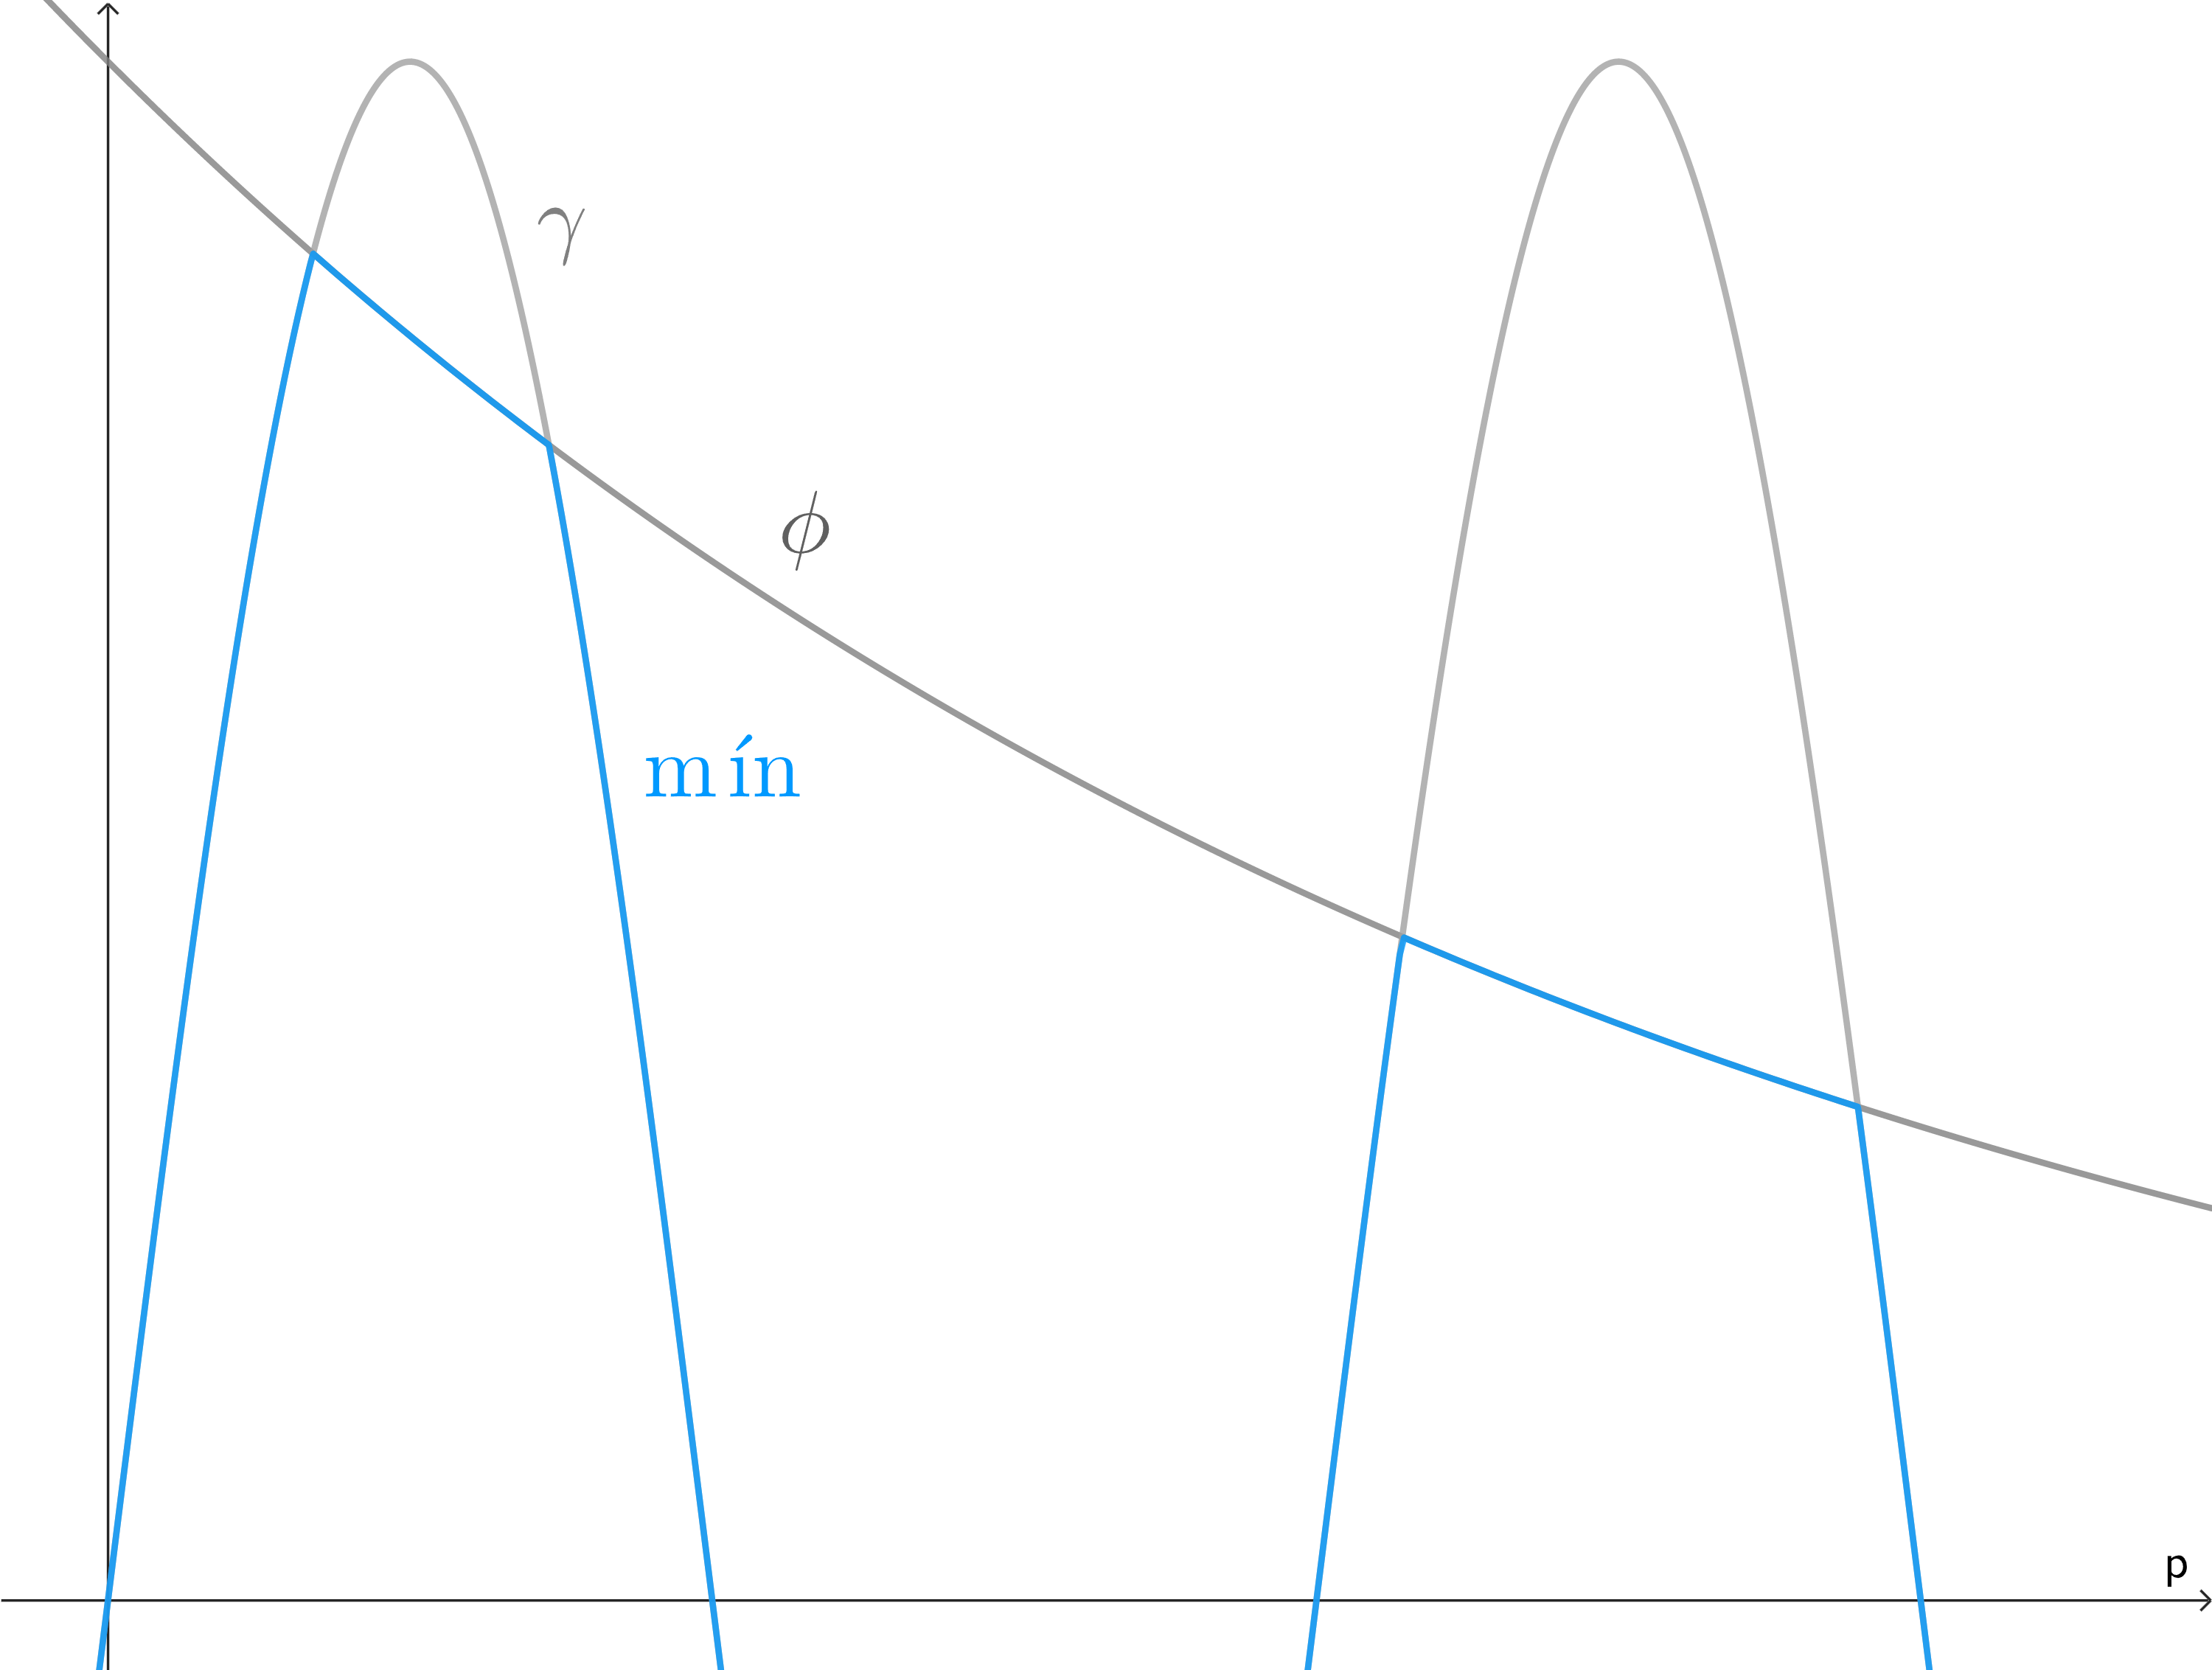
\includegraphics[width=0.75\textwidth]{Plantilla-TFG-master/img/smooth_real.png}
    \caption{Gráfica de $\Min\colon \R\to\R$}
    \label{fig:min_real}
\end{figure}

Para asegurar que $\smin$ sea continua en la frontera de $B_{k}$, imponemos la condición 
\begin{equation*}
    \omega_k(p) = 0,\ \text{para todo } p \in \delta B_{k}.
\end{equation*}
Por otro lado, es lógico que $\omega_k$ tenga su mayor influencia justo en las intersecciones, luego imponemos también 
\begin{equation*}
    \omega_k(c) = s, \text{ donde } c \in I = \{p\in\R^3 : \phi(p) = \gamma(p)\},\ s\in \R.
\end{equation*}

El valor $s$ es el que deberemos ajustar para que $\smin$ cumpla nuestros requisitos. Fijado un $p\in B_{k}$, consideramos una primera aproximación para $\omega_k$ :
\begin{equation*}
    \omega_k(p) = s\left( 1-\frac{|\phi(p)-\gamma(p)|}{k} \right)^n = \begin{cases}
        s\left( 1-\frac{\phi(p)-\gamma(p)}{k}\right)^n,\ \phi(p)>\gamma(p), \\[10pt]
        s\left( 1+\frac{\phi(p)-\gamma(p)}{k}\right)^n,\ \phi(p)\le \gamma(p)\\[10pt]
    \end{cases}  ,\ s\in\R,\ n\in\N,
\end{equation*}
donde hemos añadido el parámetro $n$ para añadir más control sobre el resultado final.\newline 
\begin{figure}[!h]
     \begin{minipage}[c]{0.49\linewidth}
        \centering
        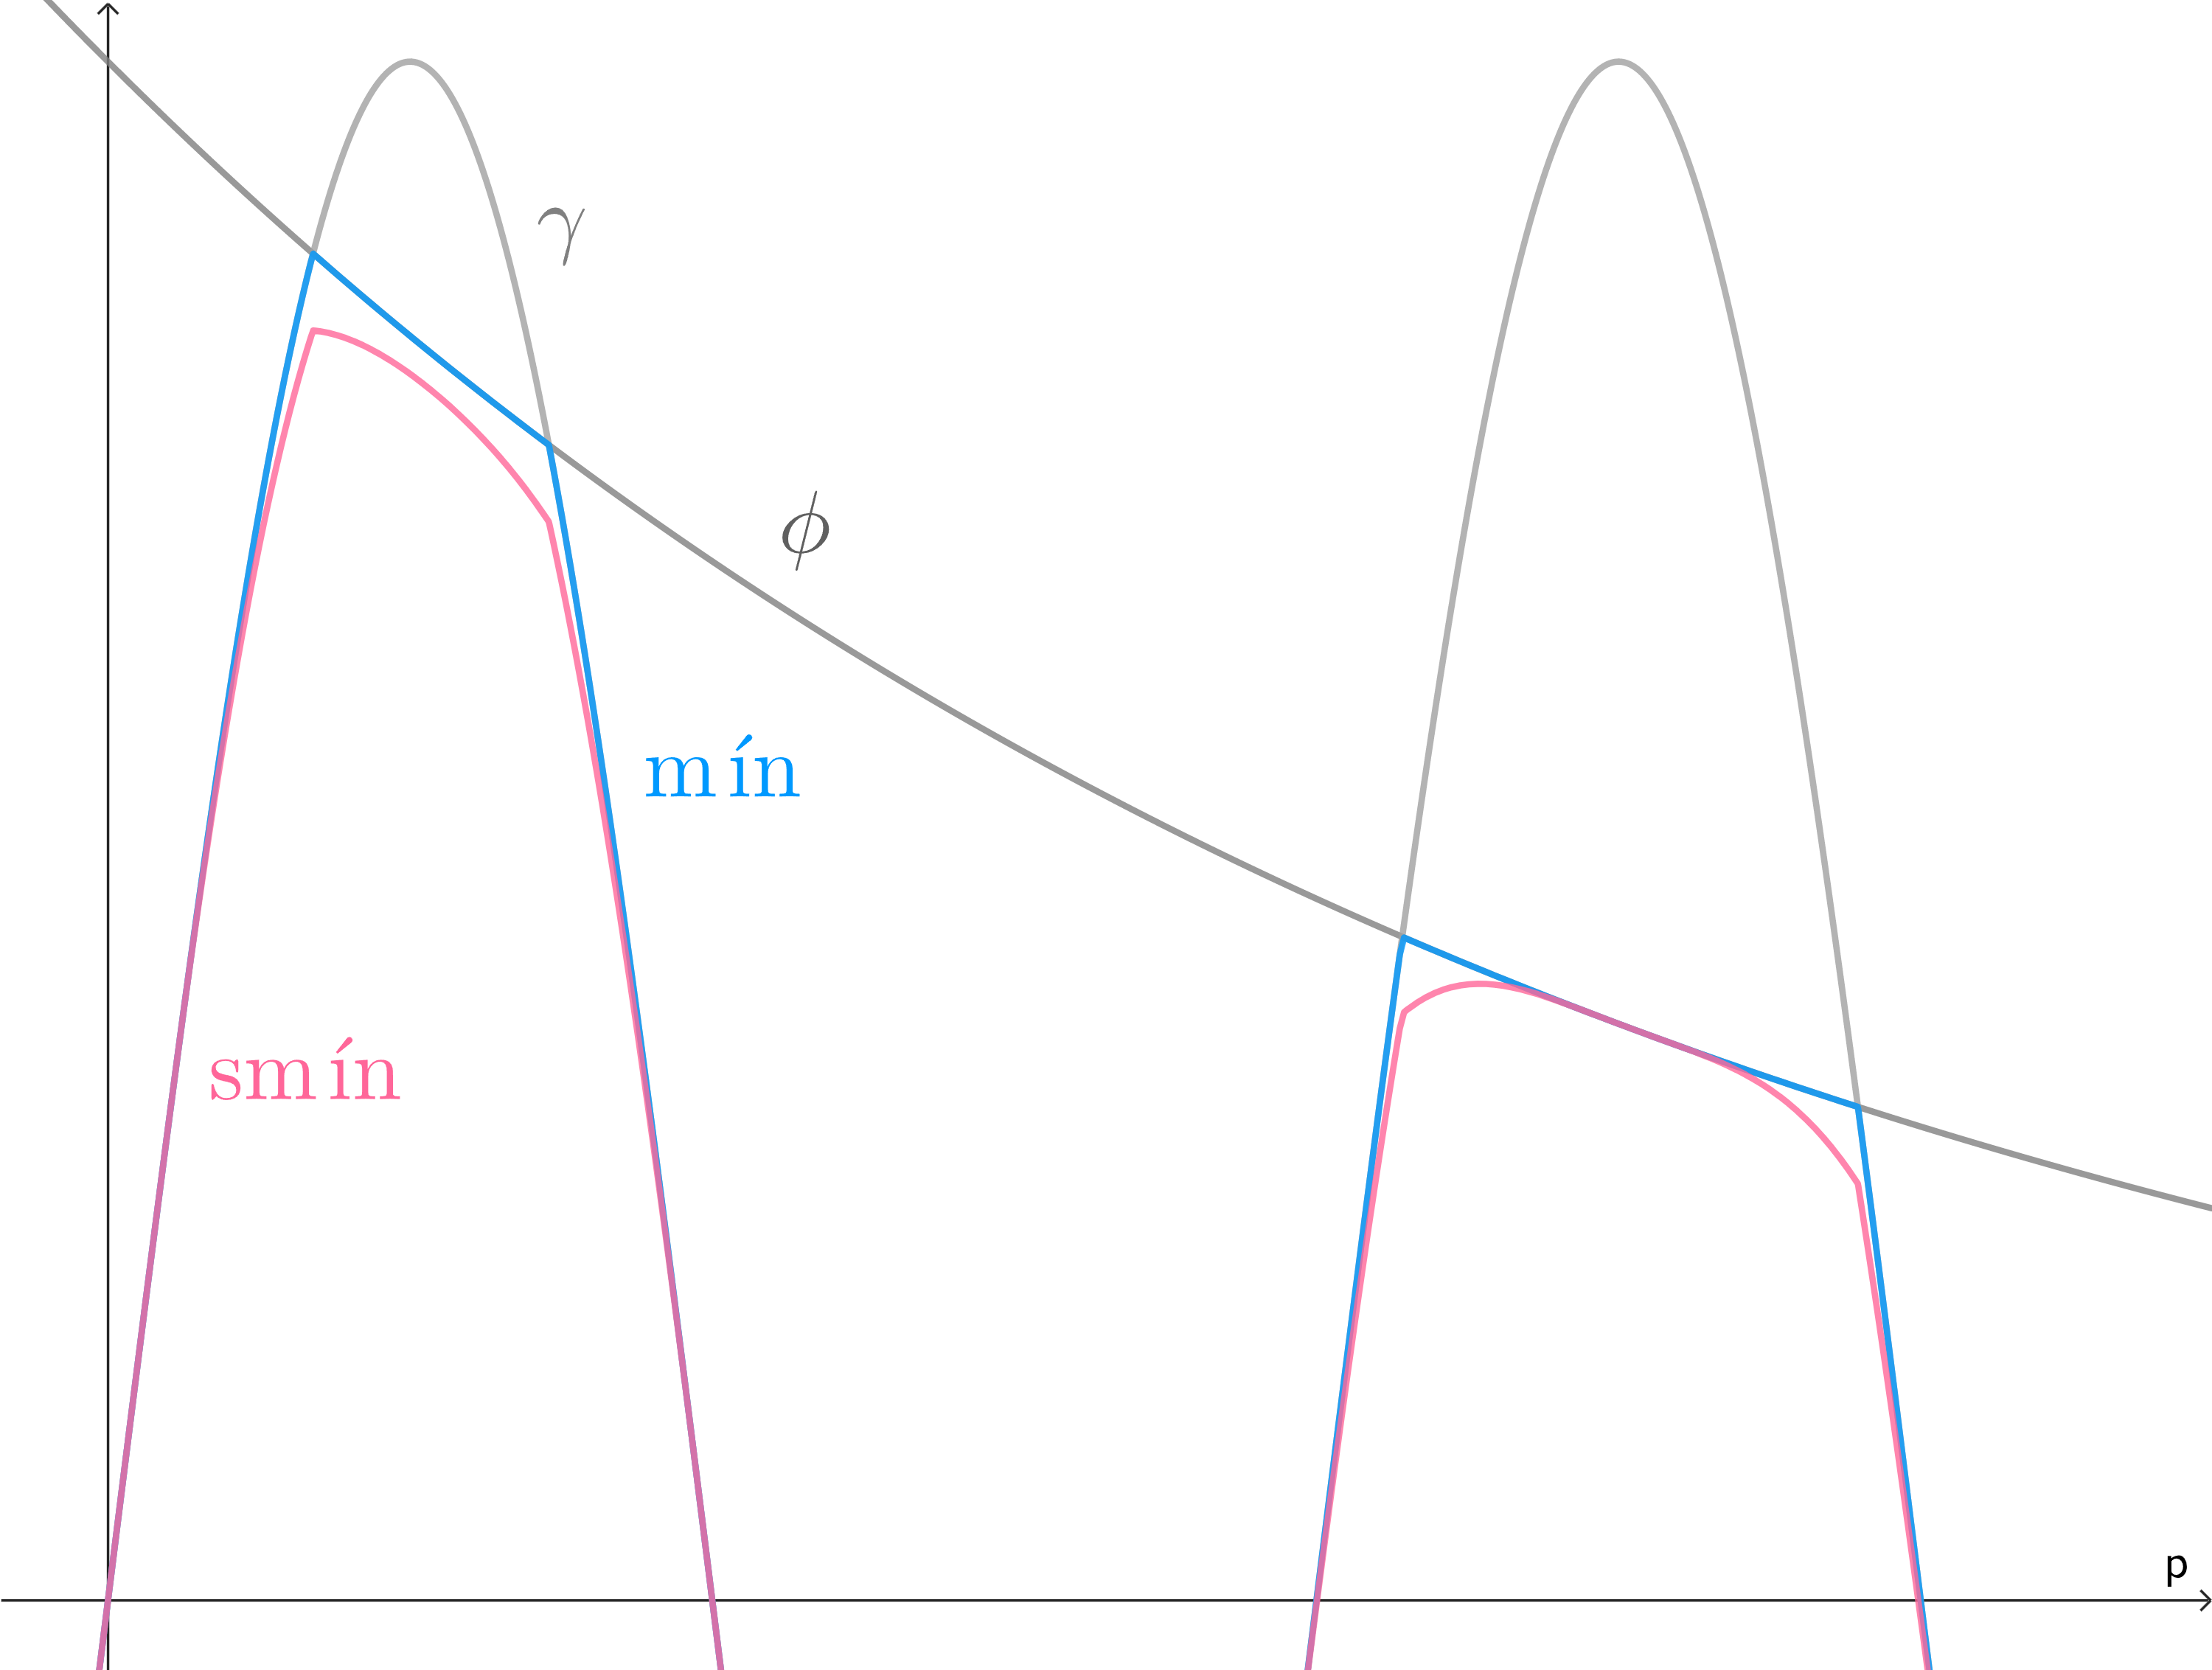
\includegraphics[width=0.95\textwidth]{Plantilla-TFG-master/img/smin_1.png}
        \caption{$k=0.6$}
     \end{minipage}
     \begin{minipage}[c]{0.49\linewidth}
        \centering
        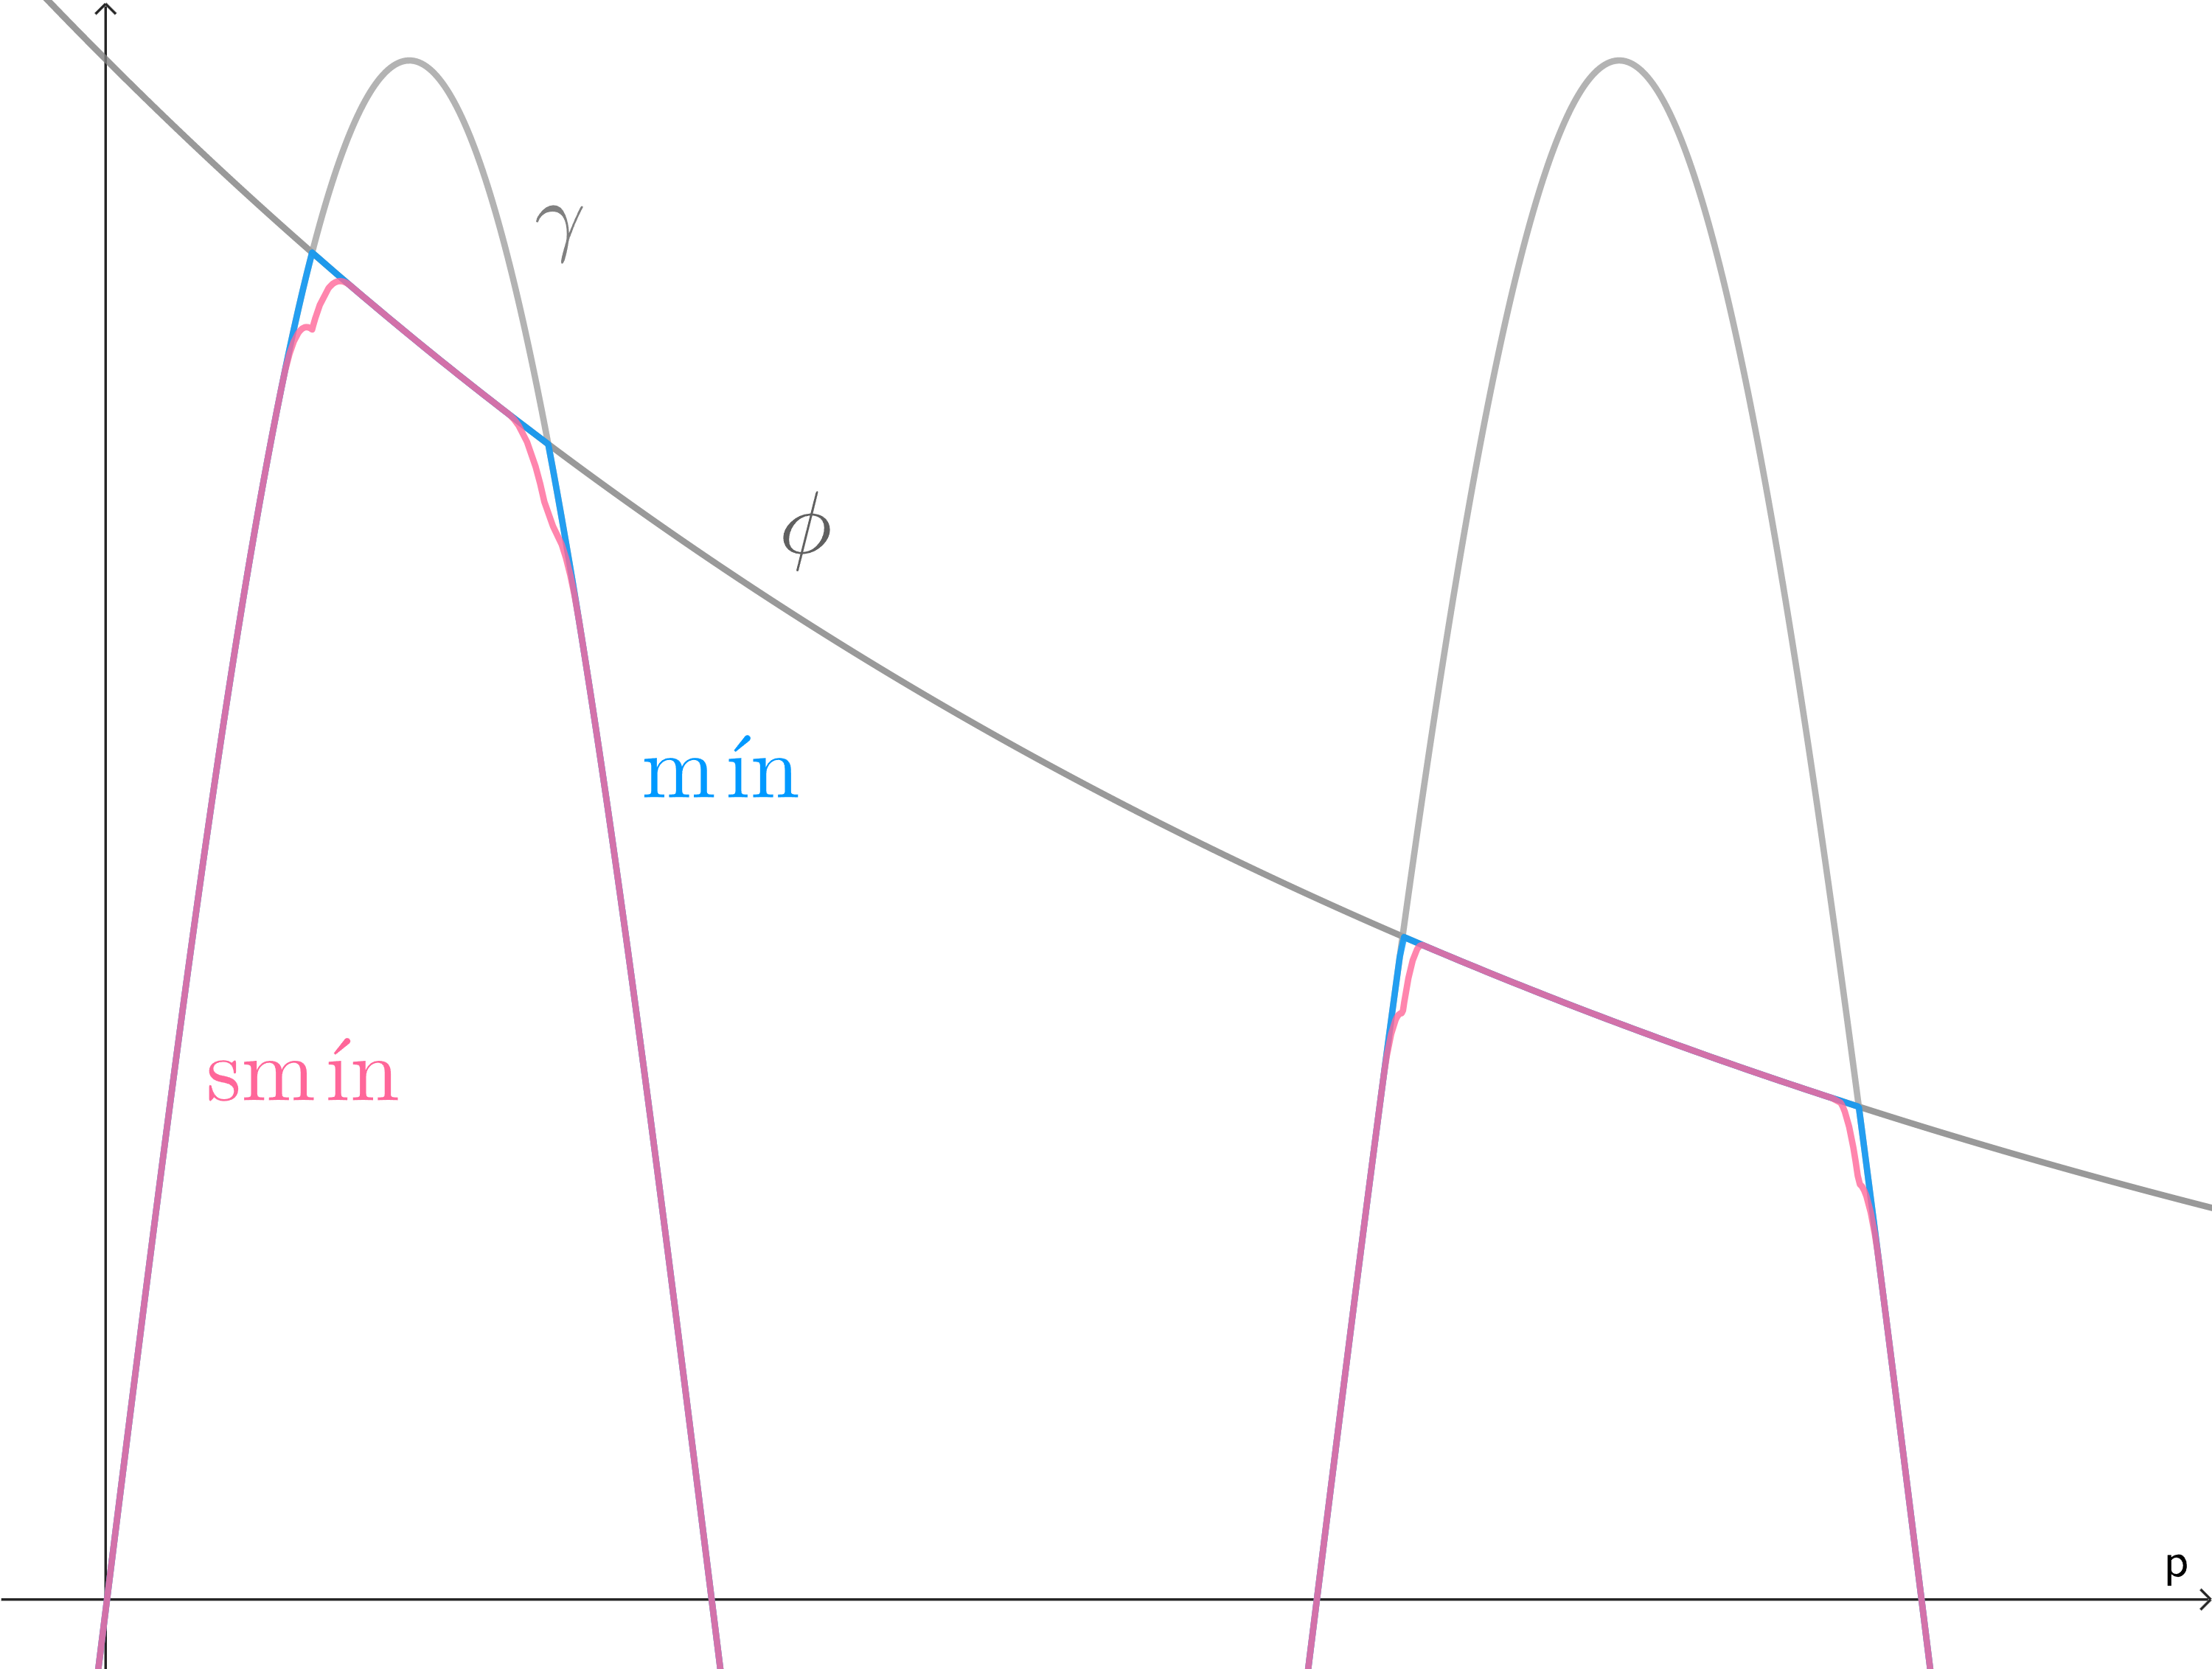
\includegraphics[width=0.95\textwidth]{Plantilla-TFG-master/img/smin_2.png}
        \caption{$k=0.1$}
     \end{minipage}
     \caption{Primera aproximación de $smin(p)$ con $s=0.05$ y $n=2$}
     \label{fig:smooth1}
\end{figure}

Nuestro objetivo es que $\smin$ tenga un aspecto natural y varíe de forma suave. Comprobemos las propiedades que debería cumplir $\smin$ para ser $\mathcal{C}^1$ en cada entorno de $B_k$. Que es continua es evidente:
\begin{equation*}
    \phi(p)=\gamma(p), \text{ luego } \frac{\phi(p)-\gamma(p)}{k} = 0, \text{ y por tanto } \omega_k(p) = s.
\end{equation*}

Otra condición necesaria es que sus derivadas parciales sean continuas. Para todo $i\in \{1,2,3\}$, estas son de la forma
\begin{align*}
    \frac{\partial \smin}{\partial x_i}(p) &= \begin{cases}
        \frac{\partial \gamma}{\partial x_i}(p)+ sn\left(1-\frac{\phi(p)-\gamma(p)}{k}\right)^{n-1}\left(\frac{ \frac{\partial \phi}{\partial p}(p)-\frac{\partial \gamma}{\partial p}(p)}{k}\right),\ \phi(p)>\gamma(p), \\[10pt] 
        \frac{\partial \phi}{\partial x_i}(p)+ sn\left(1-\frac{\phi(p)-\gamma(p)}{k}\right)^{n-1}\left(\frac{ \frac{\partial \phi}{\partial p}(p)-\frac{\partial \gamma}{\partial p}(p)}{k}\right),\ \phi(p)\le\gamma(p).
    \end{cases}
\end{align*}

Por tanto, para comprobar que las parciales son continuas cuando $\phi(p) = \gamma(p)$, para todo $i\in \{1,2,3\}$ imponemos 
\begin{align*}
     \frac{\partial \phi}{\partial x_i} - sn\left(1+\frac{\phi-\gamma}{k}\right)^{n-1}\left(\frac{\frac{\partial \phi}{\partial x_i}-\frac{\partial \gamma}{\partial x_i}}{k}\right) &= \frac{\partial \gamma}{\partial x_i} + sn\left(1-\frac{\phi-\gamma}{k}\right)^{n-1}\left(\frac{\frac{\partial \phi}{\partial x_i}-\frac{\partial \gamma}{\partial x_i}}{k}\right),\\[10pt]
     \cancel{\frac{\partial \phi}{\partial x_i} - \frac{\partial \gamma}{\partial x_i}} &= 2sn\left(1-\frac{\phi-\gamma}{k}\right)^{n-1}\left(\frac{ \cancel{\frac{\partial \phi}{\partial x_i}-\frac{\partial \gamma}{\partial x_i}}}{k}\right),\\[10pt]
     s &= \frac{k}{2n}\left(1-\frac{\phi-\gamma}{k}\right).
\end{align*}

Evaluando en $c\in I$:
\begin{align*}
    s = \frac{k}{2n}\left(1-\frac{\cancelto{0}{\phi(c)-\gamma(c)}}{k}\right), \text{ luego } s = \frac{k}{2n}.
\end{align*}
    
Hemos llegado a la expresión final
\begin{align}
    \label{eq:correccion}
    \omega_k(p) &= \begin{cases}
        \frac{k}{2n}\left( 1-\frac{|\phi(p)-\gamma(p)|}{k} \right)^n,\ &|\phi(p)-\gamma(p)|\le k,\\[10pt]
        0,\ &\text{ otro caso },
    \end{cases}\\[10pt] &= \frac{\Max\left( k - |\phi(p) - \gamma(p)|, 0\right)^n}{2n\cdot k^{n-1}}  ,\ s\in\R,\ n\in\N. 
\end{align}

Podemos observar los resultados en la \autoref{fig:smooth2}. Finalmente, para obtener una versión suavizada del máximo, es fácil comprobar que 
\begin{align*}
      \smax_{\phi,\gamma}\colon \R^3&\to \R,\\
      p &\mapsto -\smin_{-\phi,-\gamma}(p).
\end{align*}

Con estos resultados, para que la transición de una superficie a otra en la \autoref{p:boolean} sea gradual basta con sustituir las versiones clásicas de las funciones máximo y mínimo por las que acabamos de obtener.  
\begin{figure}[!h]
     \begin{minipage}[c]{0.49\linewidth}
        \centering
        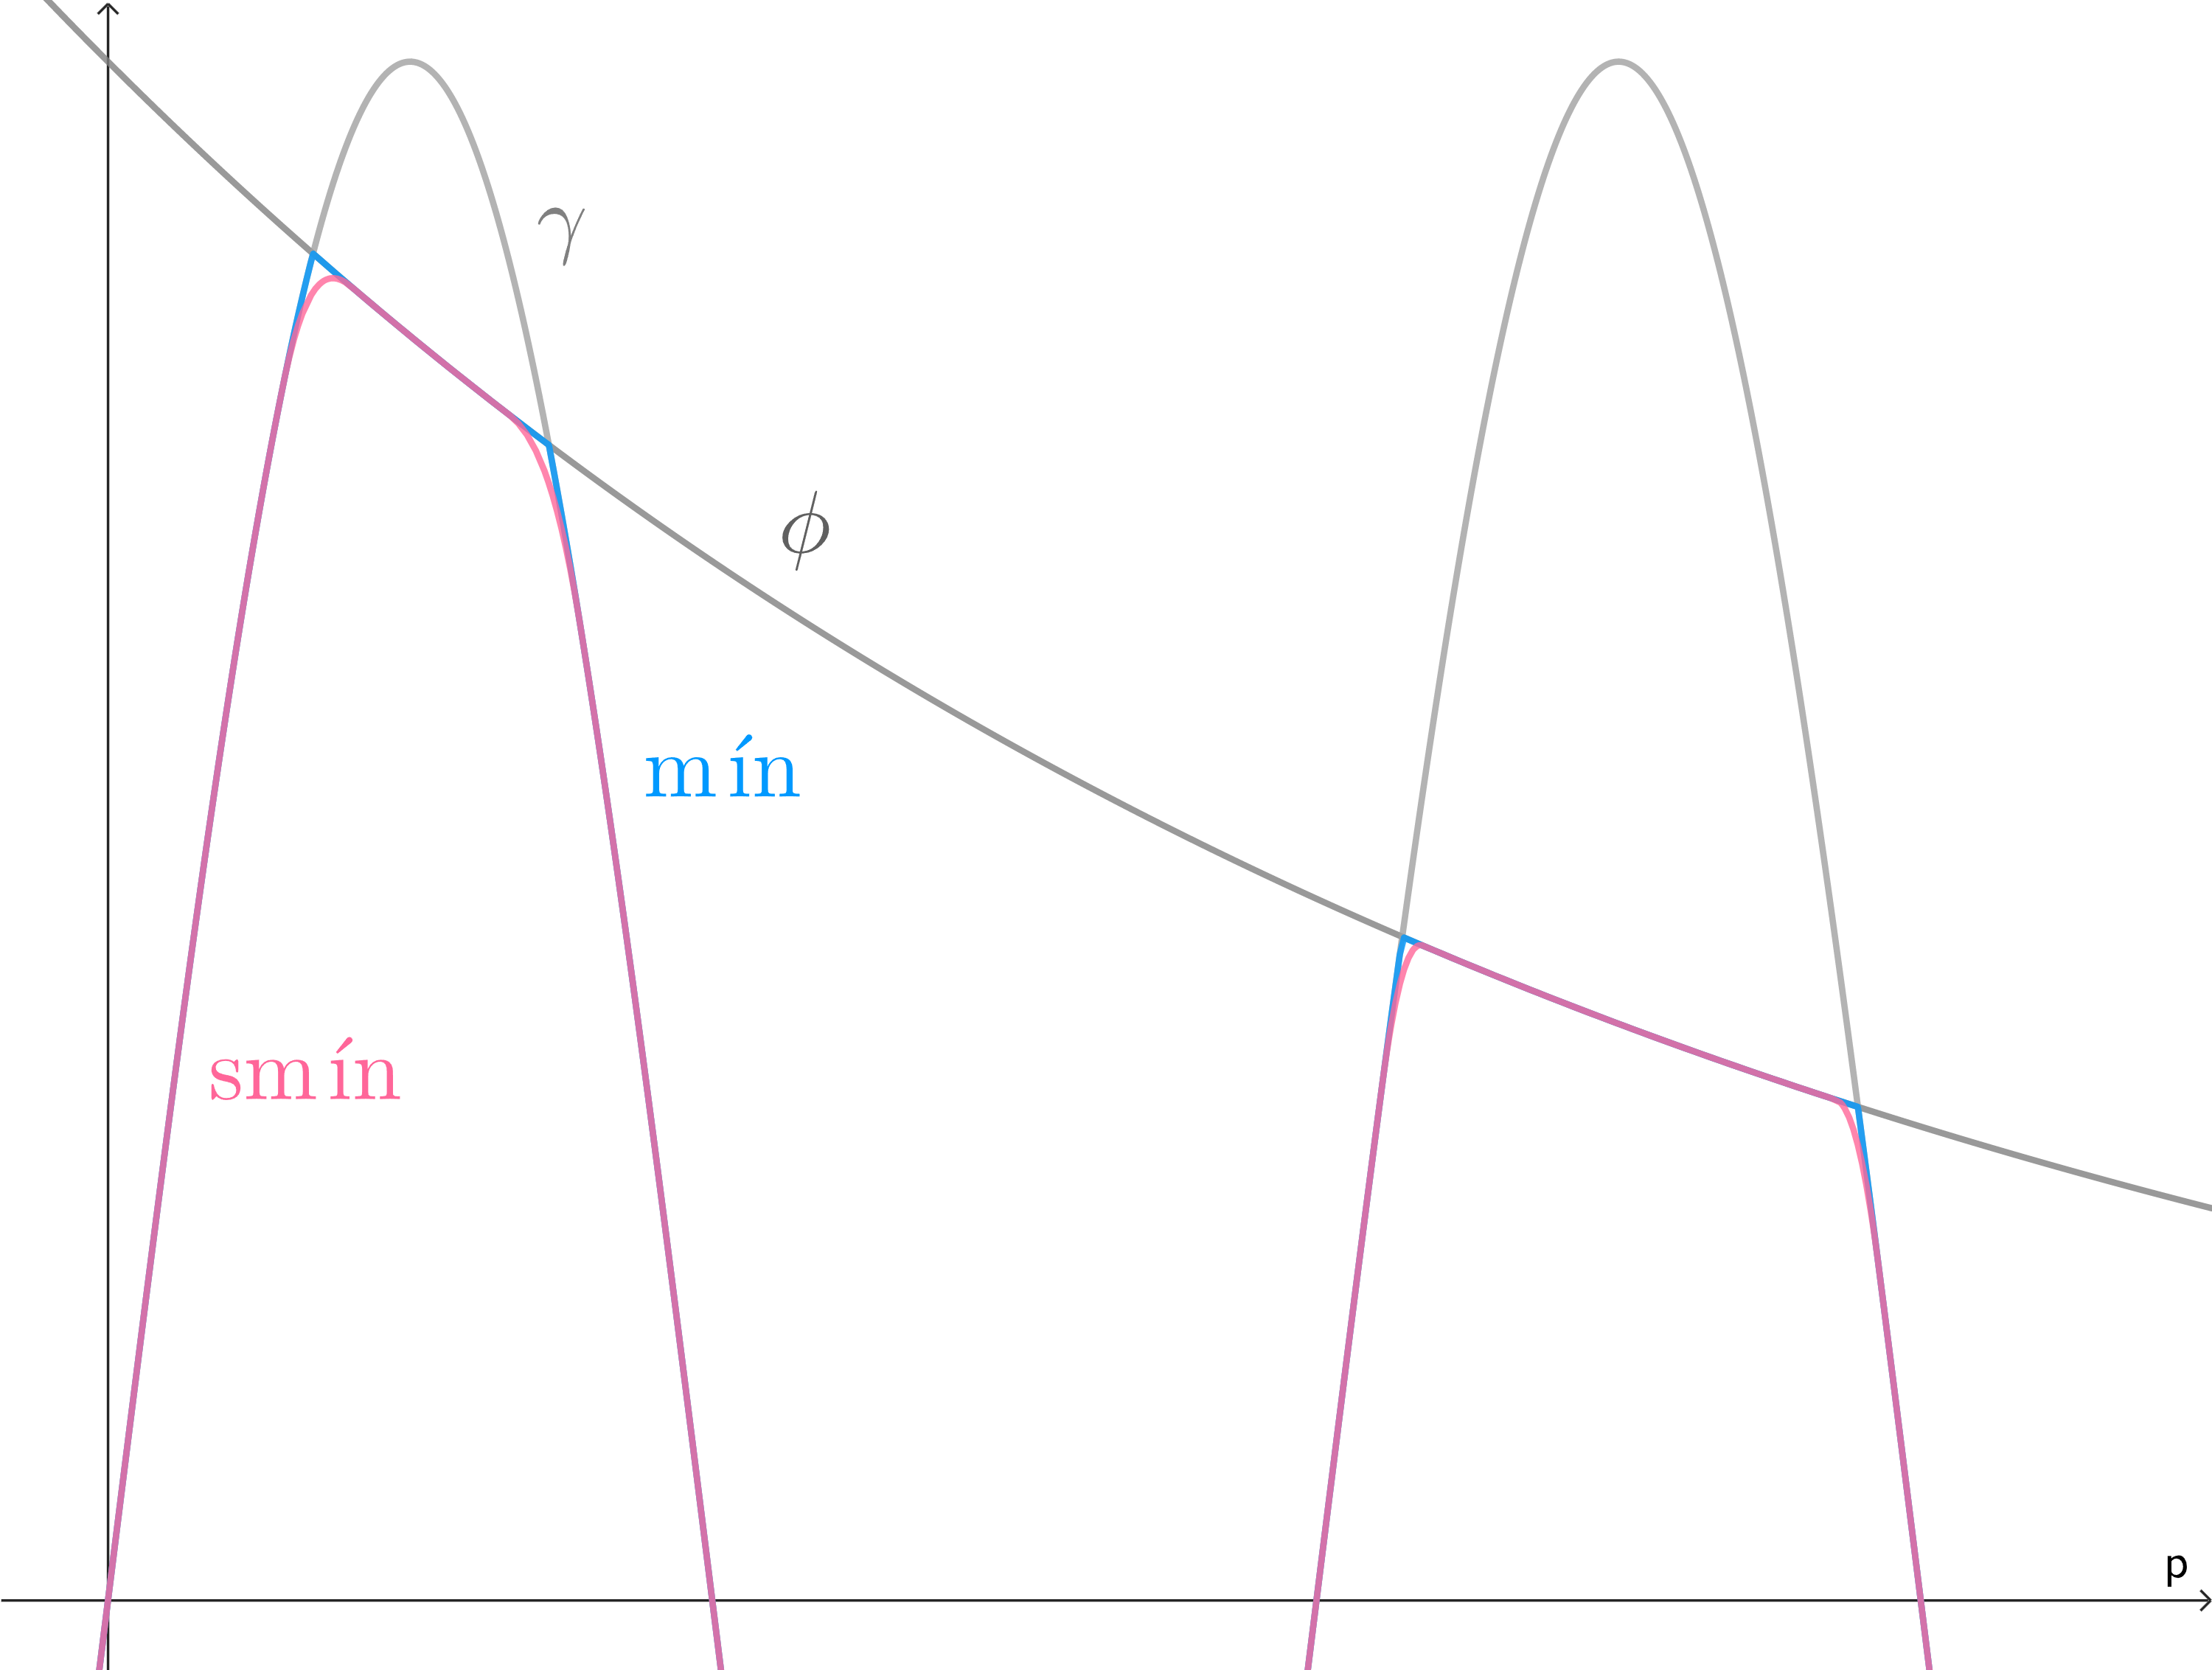
\includegraphics[width=0.95\textwidth]{Plantilla-TFG-master/img/smin_3.png}
        \caption{$k=0.1,\ n=2$}
     \end{minipage}
     \begin{minipage}[c]{0.49\linewidth}
        \centering
        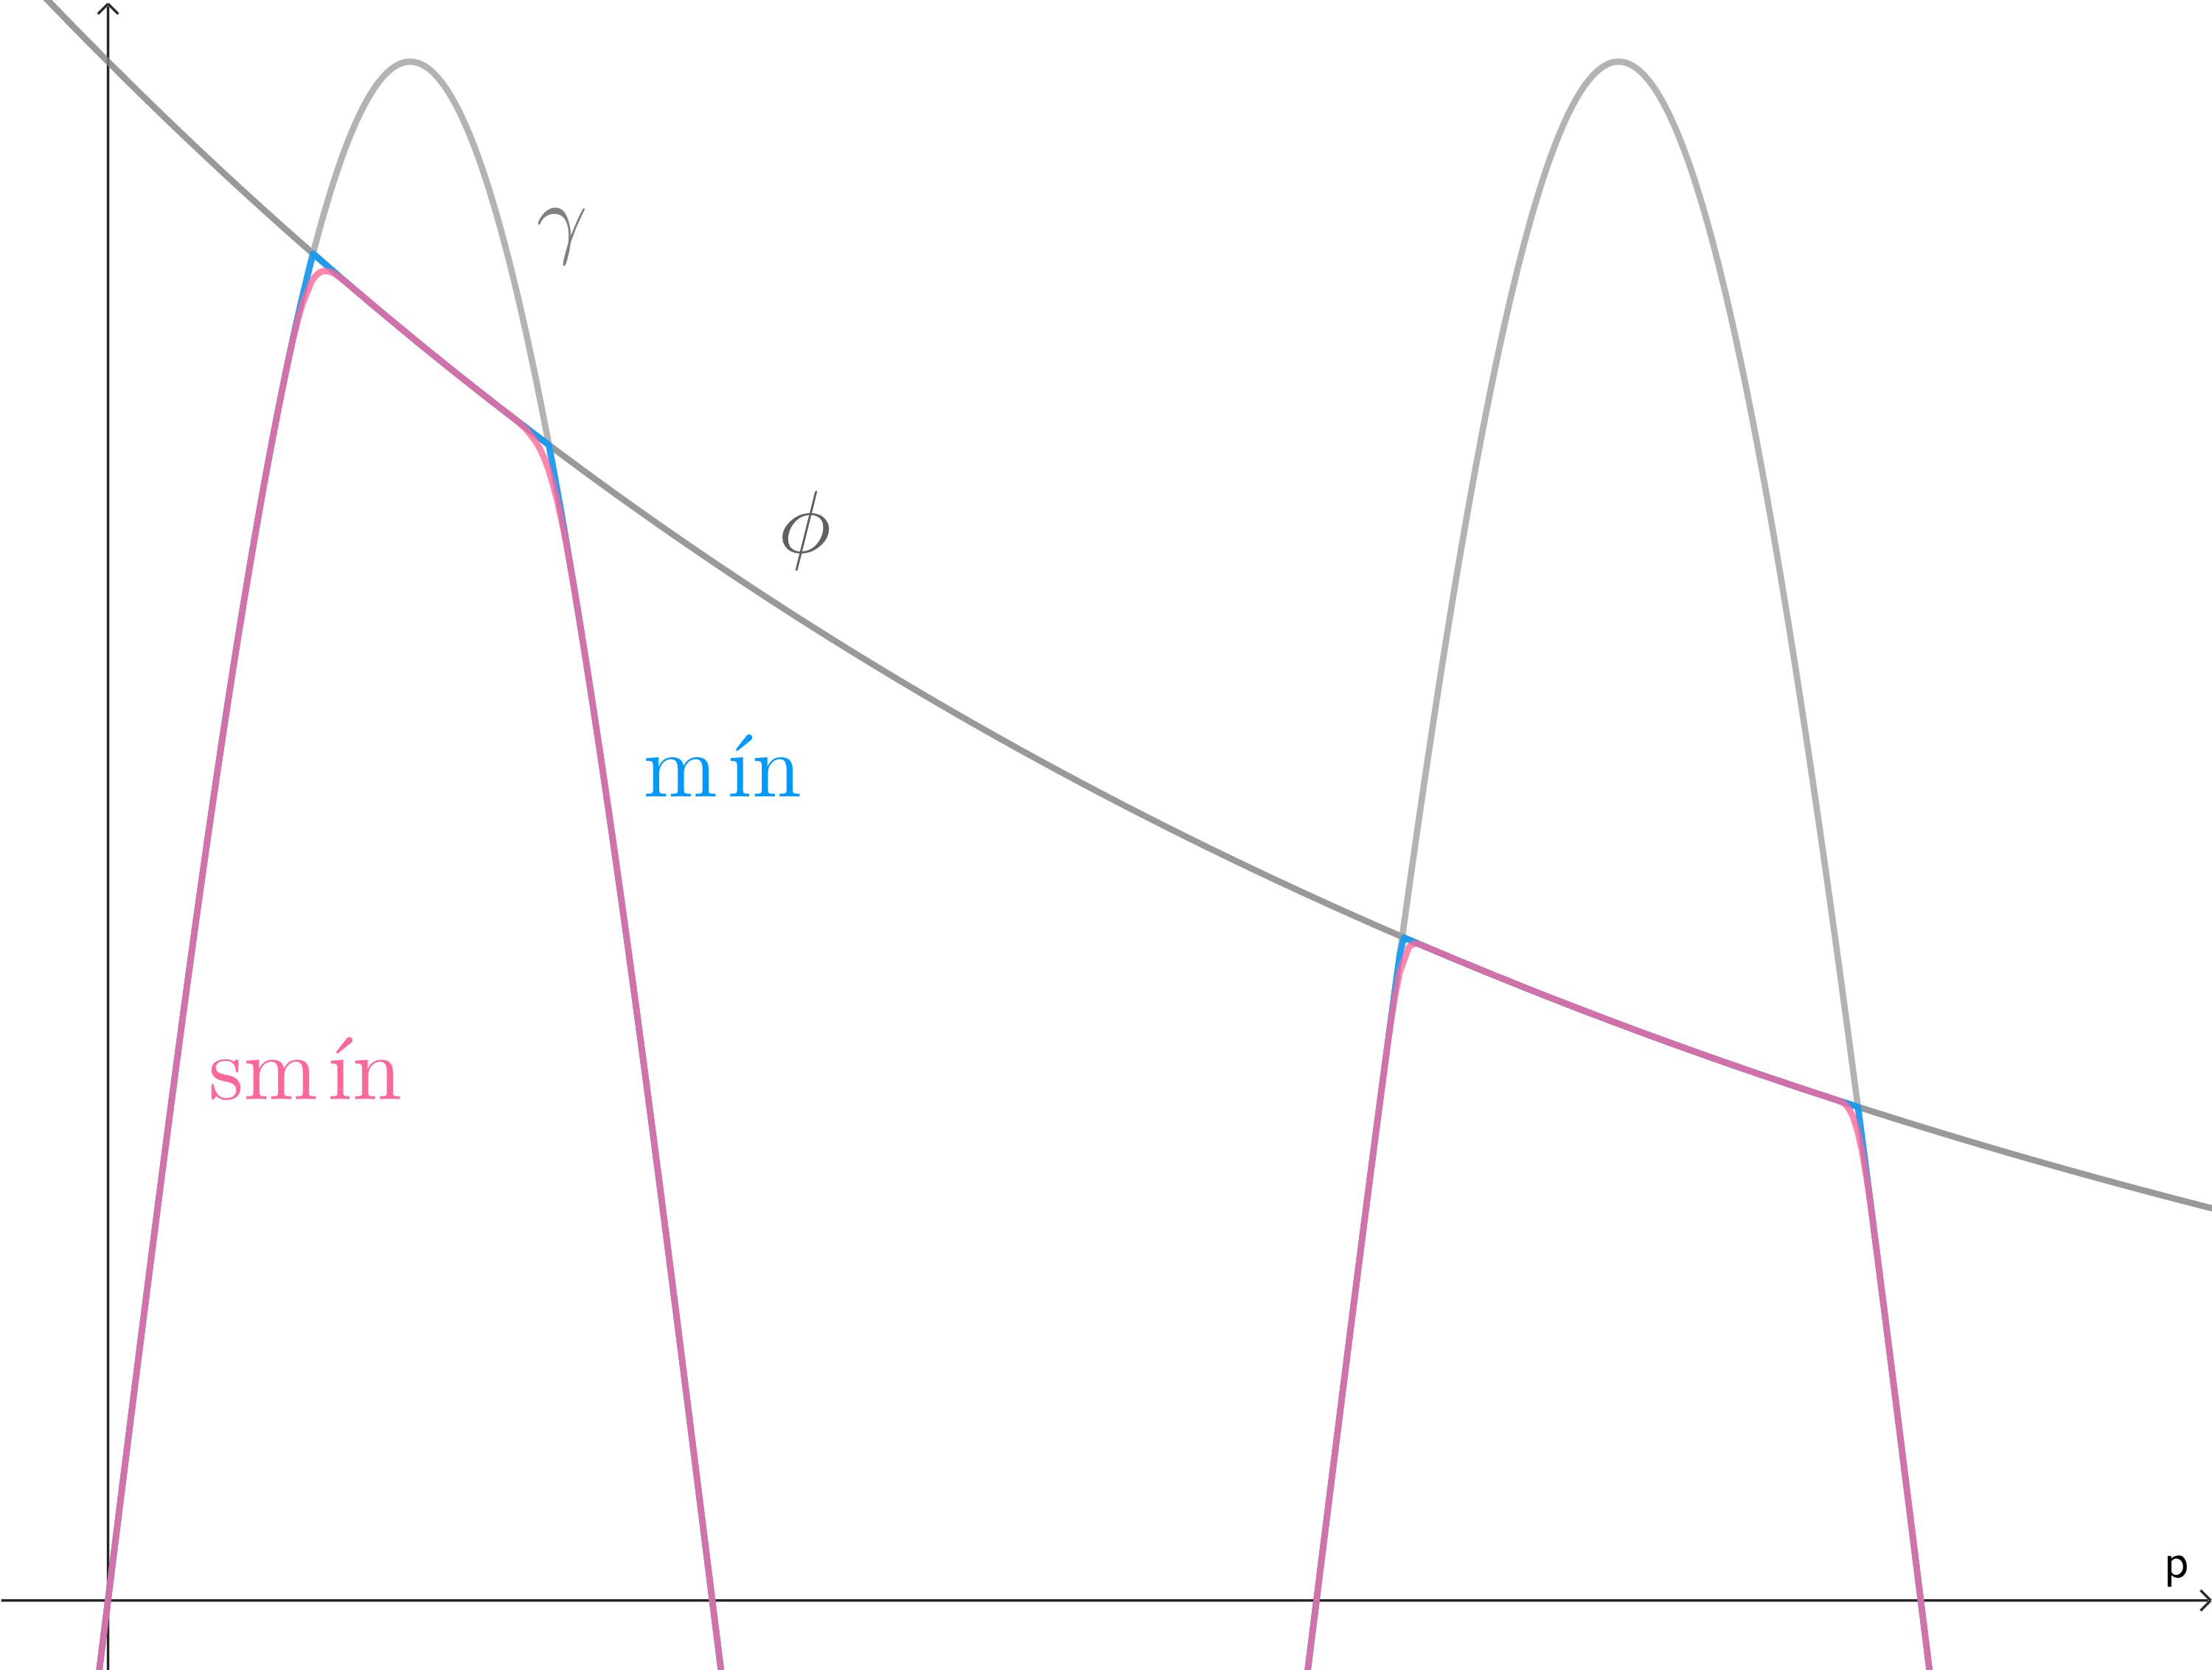
\includegraphics[width=0.95\textwidth]{Plantilla-TFG-master/img/smin_4.png}
        \caption{$k=0.1,\ n=3$}
     \end{minipage}
     \caption{Resultado final de $smin(p)$ }
     \label{fig:smooth2}
\end{figure}





% Por tanto, dadas $\phi$ y $\gamma$, queremos obtener una versión suavizada de $\Min(\phi,\gamma)$ usando interpolación lineal, que llamaremos $\smin$ y tendrá la forma
% \begin{align*}
%           \smin\colon \R^3 &\to \R^3.\\
%           p &\mapsto h(p)\cdot \phi(p) + (1-h(p))\gamma(p) \text{, donde } h \colon \R^3 \to [0,1].
%     \end{align*}


% Pasamos a buscar $h$. Solo queremos modificar la función en los entornos de los puntos en los que intersecan $\phi$ y $\gamma$, de forma que para el resto de puntos debería ser $h=\{0,1\}$. Los puntos de intersección vienen dados como las soluciones de $m(p)=\gamma(p) - \phi(p)$. Podemos además acotar $m(p)$ en el intervalo $[0,1]$ usando $\Min$ y $\Max$, obteniendo un candidato a valor de $h(p)$:
% \begin{equation}
%     \Min\left(\Max\left(\phi(p)-\gamma(p),0\right),1\right) = \Min\left(\Max\left(m(p),0\right),1\right) \in [0,1]
% \end{equation}

% Sin embargo, podemos ver que la interpolación comienza justo en la intersección, mientras que nos gustaría que esto ocurriese antes. Modificamos la expresión anterior para hacer que la intersección sea el punto medio de la interpolación ($h=0.5$):
% \begin{equation}
%    \Min\left(\Max\left(m(p) + \frac{1}{2},0\right),1\right)
% \end{equation}

% Podemos ver los resultados de esta primera aproximación en la \autoref{fig:smooth1}.

% \begin{figure}[!h]
%      \begin{minipage}[c]{0.49\linewidth}
%         \centering
%         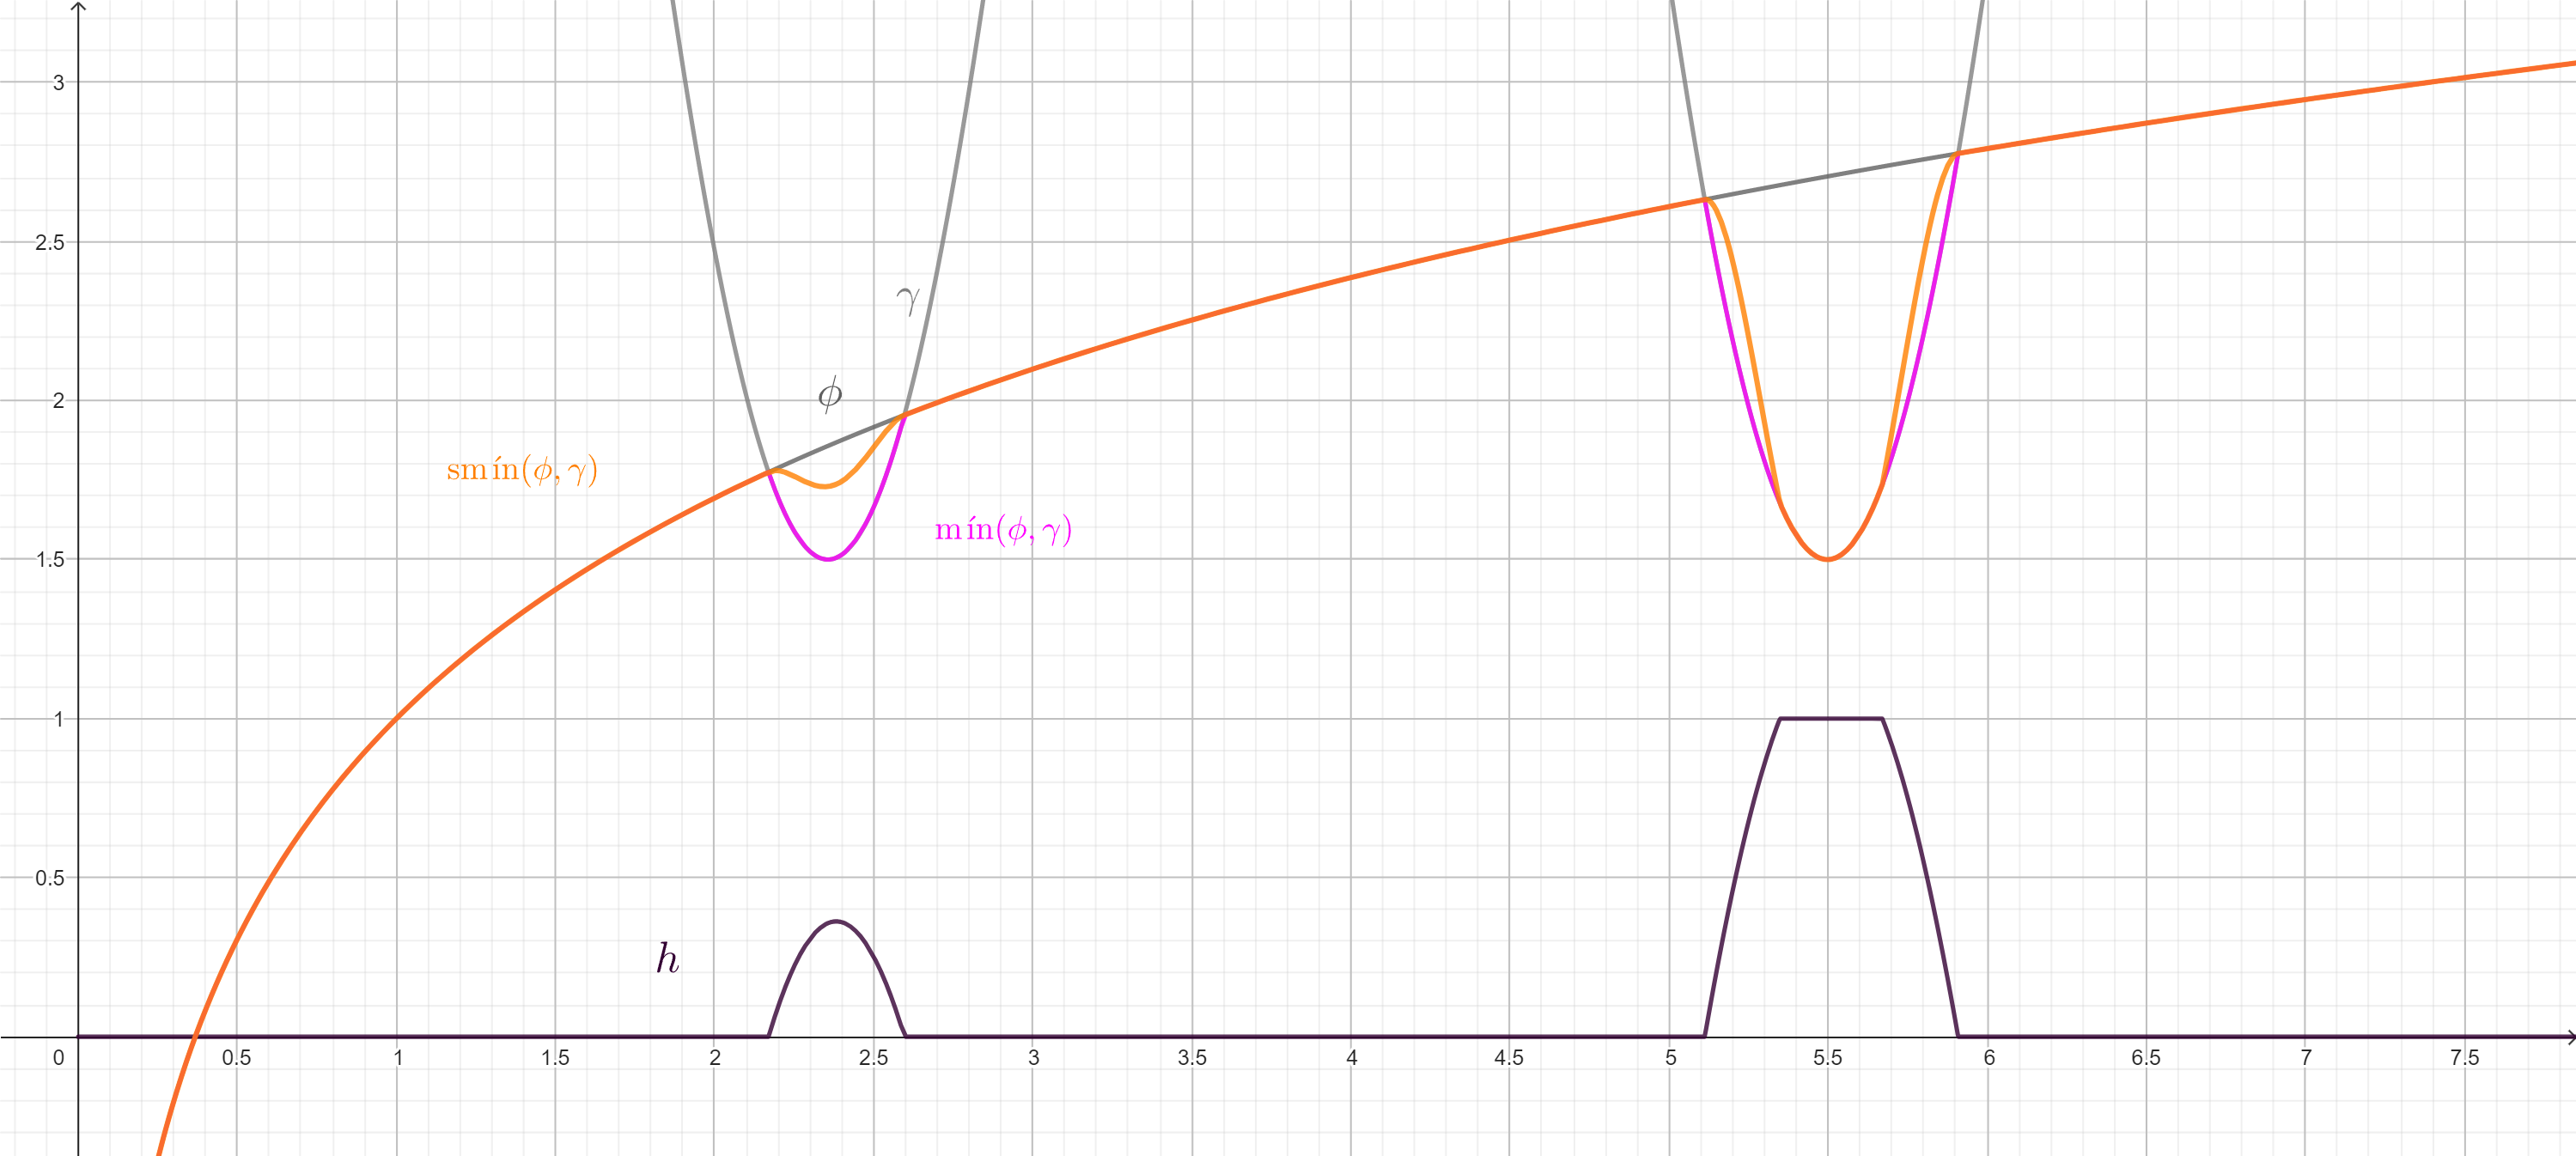
\includegraphics[width=0.95\textwidth]{Plantilla-TFG-master/img/smoothV1_a.png}
%         \caption{$h(p)=0$ en la intersección}
%      \end{minipage}
%      \begin{minipage}[c]{0.49\linewidth}
%         \centering
%         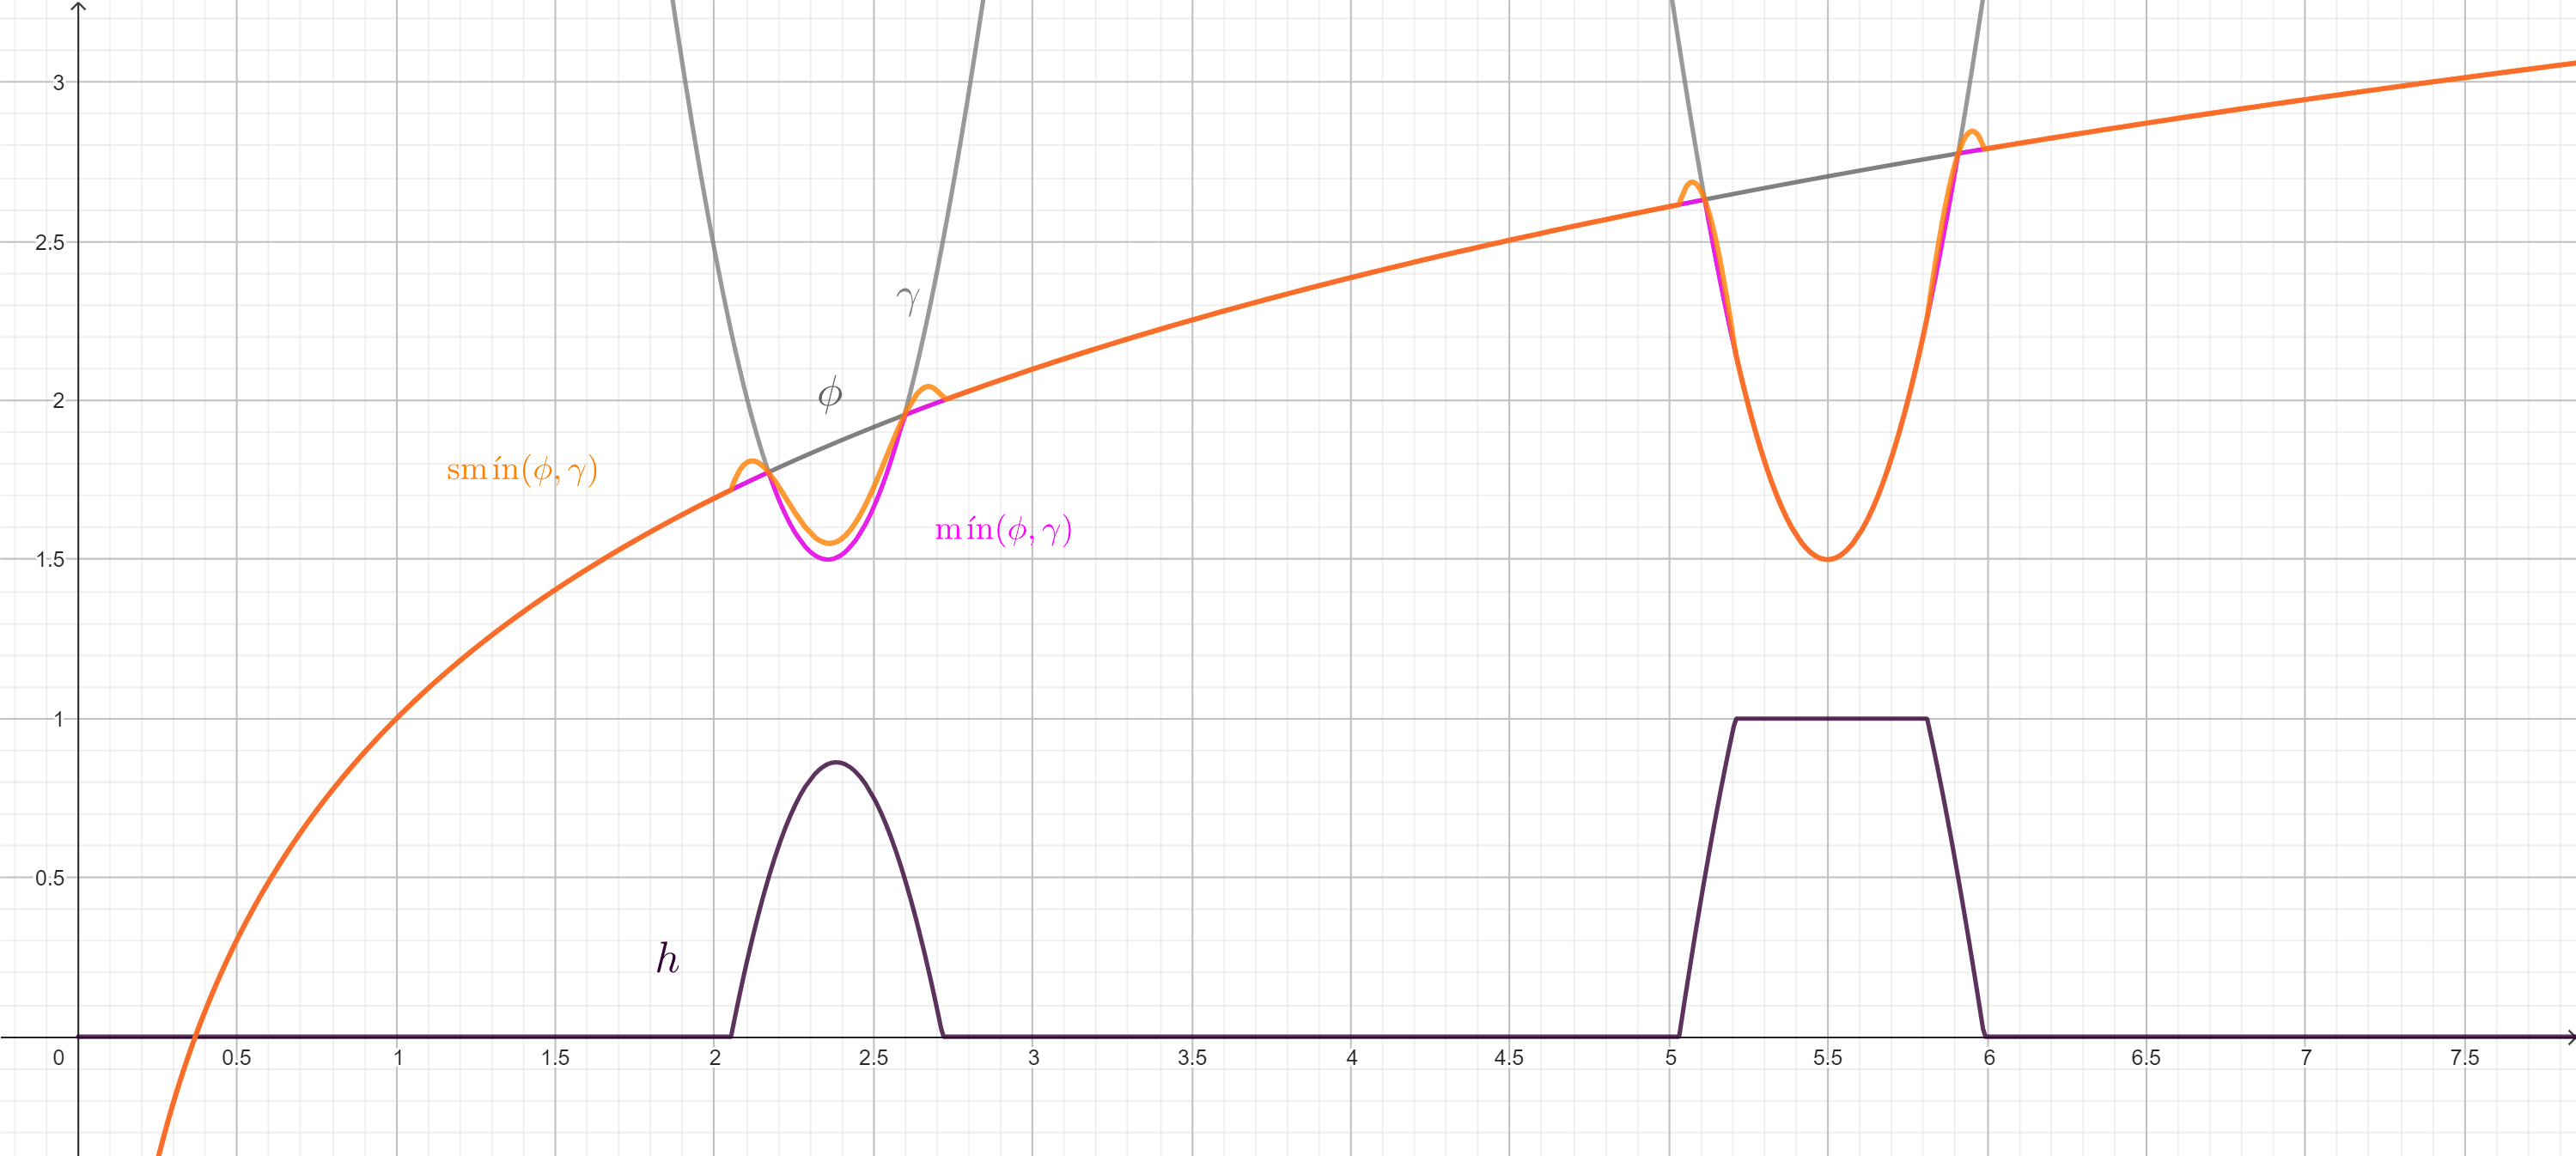
\includegraphics[width=0.95\textwidth]{Plantilla-TFG-master/img/smoothV1_b.png}
%         \caption{$h(p)=0.5$ en la intersección}
%      \end{minipage}
%      \caption{Primera aproximación de la obtención de $h(p)$}
%      \label{fig:smooth1}
% \end{figure}

% Observamos que ahora tenemos un nuevo problema

\begin{definicion}[Operaciones Booleanas Suavizadas]
    Sean $A$ y $B$ isosuperficies generadas por $\phi$ y $\gamma$ respectivamente. La función $\mu$ define la isosuperficie para las siguientes operaciones.
    \begin{itemize}
        \item \textbf{Unión suavizada: } $\mu_{unionS}(p) = \Min(\phi(p),\gamma(p)) - \frac{\Max\left( k - |\phi(p) - \gamma(p)|, 0\right)^n}{2n\cdot k^{n-1}}$.
        \item \textbf{Intersección suavizada: } $\mu_{interS}(p) = -\Min(-\phi(p),-\gamma(p)) + \frac{\Max\left( k - |\phi(p) - \gamma(p)|, 0\right)^n}{2n\cdot k^{n-1}}$.
        \item \textbf{Diferencia suavizada: } $\mu_{difS}(p) = -\Min(-\phi(p),\gamma(p)) + \frac{\Max\left( k - |\phi(p) + \gamma(p)|, 0\right)^n}{2n\cdot k^{n-1}}$.
    \end{itemize}
    La constante $k\in \R^+_0$ controla la influencia del suavizado.        
\end{definicion}

Observamos que los operadores definidos en la \autoref{p:boolean} no son más que un caso particular de estos últimos cuando $k$ tiende a cero. Este método para obtener una versión suavizada de las funciones mínimo y máximo no es el único. Hemos elegido debido a que las funciones obtenidas tienen asociado un coste computacional. Además, su deducción es bastante natural y el efecto que tiene el valor $k$ sobre el resultado final es intuitivo para el usuario. En el artículo que hemos mencionado al inicio de la sección, Íñigo Quílez \cite{article:smooth} presenta otras tres alternativas a esta versión, a la cual él se refiere como \qq{mínimo suavizado polinomial}, y que también son compatibles con \textit{raymarching}.
\begin{itemize}
    \item \textbf{Mínimo suavizado exponencial:} $\smin_{\phi,\gamma}(p) = \frac{-\log_2\left( 2^{-k\phi(p)} + 2^{-k\gamma(p)} ) \right)}{k}$.
    \item \textbf{Mínimo suavizado potencial:} $\smin_{\phi,\gamma}(p) = \left(\frac{\phi(p)^k \cdot \gamma(p)^k}{\phi(p)^k + \gamma(p)^k}\right)^{1/k}$.
    \item \textbf{Mínimo suavizado por raíz:} $\smin_{\phi,\gamma}(p) = \frac{\phi(p) + \gamma(p) - \sqrt{(\phi(p)-\gamma(p))^2+k}}{2}$.
\end{itemize}

La principal ventaja de la versión polinomial respecto a estas es que es la más rápida al ser sus cálculos computacionalmente más baratos. Por otro lado tanto la exponencial como la potencial permiten ser adaptadas fácilmente para calcular el mínimo de un conjunto arbitrario de puntos, útil cuando se trabaja con patrones de voronoi o nubes de puntos. Además, la versión exponencial produce siempre el mismo resultado independientemente del orden en el que se aplique. Es decir,
\begin{equation*}
    \smin_{a,\smin_{b,c}} = \smin_{b,\smin_{a,c}}.
\end{equation*}

En la \autoref{fig:smoothVS} podemos ver un ejemplo de uso de estas versiones, en las que además se ha usado el valor de $w_k$ de la ecuación \autoref{eq:correccion} para interpolar la componente difusa de ambas primitivas usando el método \texttt{mix} de GLSL. Como vemos, no hay diferencias notables entre las distintas versiones, así que nos quedaremos con el método más eficiente: el polinómico.
\begin{figure}[htbp]
    \centering
    \begin{subfigure}[b]{0.25\textwidth}
        \centering
        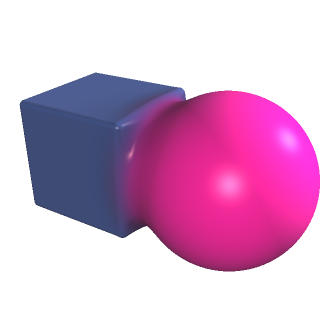
\includegraphics[width=\textwidth]{Plantilla-TFG-master/img/unionMethodOG.png}
        \caption{Polinomial, $k=1.5$}
    \end{subfigure}
    \hfill
    \begin{subfigure}[b]{0.25\textwidth}
        \centering
        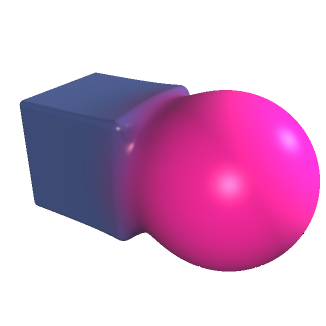
\includegraphics[width=\textwidth]{Plantilla-TFG-master/img/unionMethodExp.png}
        \caption{Exponencial, $k=2.5$}
    \end{subfigure}
    \hfill
    \begin{subfigure}[b]{0.25\textwidth}
        \centering
        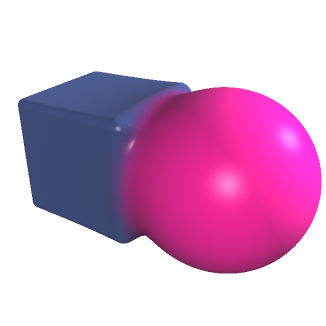
\includegraphics[width=\textwidth]{Plantilla-TFG-master/img/unionMethodRoot.png}
        \caption{Raíz, $k=1$}
    \end{subfigure}
    
    \caption{Diferentes versiones de la unión suavizada}
    \label{fig:smoothVS}
\end{figure}

\subsection{Operaciones afines}
Pasamos ahora a estudiar otro tipo de operaciones que nos permitirán aplicar movimientos rígidos y cambios de escala a las primitivas en la escena. A diferencia de los operadores booleanos, que eran binarios, estas operaciones se aplican a una única primitiva. Su funcionamiento se basará en aplicar una transformación $t:\R^3\to \R^3$ a cada punto de la isosuperficie $S_{\phi}$ para obtener la transformada $S_{\gamma}$. Si queremos saber si un punto $q\in\R^3$ está en $S_{\gamma}$, tenemos que comprobar si su preimagen por la transformación pertenece a $S_{\phi}$. Por tanto, bastará evaluar la SDF original en $t^{-1}(p)$:
\begin{equation*}
    \gamma(p) = \phi(t^{-1}(p)).
\end{equation*}

Este razonamiento funciona bien para transformaciones como las traslaciones o rotaciones, que son movimientos rígidos y mantienen las distancias. Sin embargo, este no es el caso del escalado, ya que si tomamos $l(p) = sp$ con $s\in \R^+_0$
\begin{equation*}
    \Vert p-p'\Vert = d, \text{ luego }  \Vert l(p)-l(p')\Vert = \Vert sp-sp'\Vert = s\Vert p-p'\Vert = s\cdot d,\  \text{ donde } p,p' \in S_{\phi}.
\end{equation*}
Como las distancias se escalan, deberemos hacer lo propio con la función que genere la nueva isosuperficie, aplicándole el mismo factor de escalado $s$ como muestra la \autoref{d:afines}.

\begin{definicion}[Operaciones afines]\label{d:afines}
    Sea $A$ una isosuperficie. Definimos las SDFs para las siguientes operaciones.
    \begin{itemize}
        \item \textbf{Traslación de vector $\boldsymbol{v\in R^3}$: } $\sdf_{traslacion}(p) = \sdf_{A}(p - v)$.
        \item \textbf{Escalado uniforme de dimensiones $\boldsymbol{(s,s,s)\in \R^3}$: } $\sdf_{escalado}(p) = \sdf_{A}(p/s)\cdot s$.
        \item \textbf{Rotaciones de ángulo $\boldsymbol{\alpha\in \R}$ sobre los ejes $\boldsymbol{x,y,z}$: }
        \begin{align*}
            \sdf_{rotX}(p) &= \mu_{A}(R_x^{-1}(\alpha)\cdot p^t),\ \text{donde } R_x(\alpha) = 
            \begin{pmatrix}
                1&0&0\\
                0&\cos(\alpha) & -\sin(\alpha) \\
                0&\sin(\alpha) & \cos(\alpha) 
                \end{pmatrix},\\[10pt] 
            \sdf_{rotY}(p) &= \mu_{A}(R_y^{-1}(\alpha)\cdot p^t),\ \text{donde } R_y(\alpha) = \begin{pmatrix}
            \cos(\alpha) &0& \sin(\alpha)\\
            0&1&0\\
            -\sin(\alpha) &0& \cos(\alpha) 
            \end{pmatrix},\\[10pt]
            \sdf_{rotZ}(p) &= \mu_{A}(R_z^{-1}(\alpha)\cdot p^t),\ \text{donde } R_z(\alpha) = \begin{pmatrix}
            \cos(\alpha) & -\sin(\alpha) & 0\\
            \sin(\alpha) & \cos(\alpha) & 0\\
            0&0&1
            \end{pmatrix}.
        \end{align*}
    \end{itemize}
\end{definicion}

Observamos que en este caso sí que obtenemos funciones distancia con signo como resultado, al contrario de lo que ocurría con las operaciones booleanas.
\begin{figure}[ht!]
    \centering
    \begin{subfigure}[b]{0.24\textwidth}
        \centering
        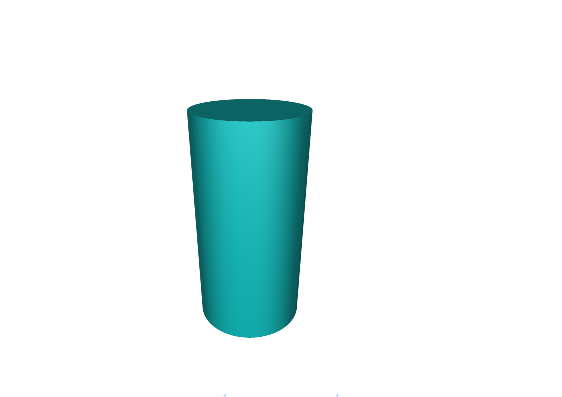
\includegraphics[width=\textwidth]{Plantilla-TFG-master/img/afin_og.png}
        \caption{Original}
    \end{subfigure}
    \hfill
    \begin{subfigure}[b]{0.24\textwidth}
        \centering
        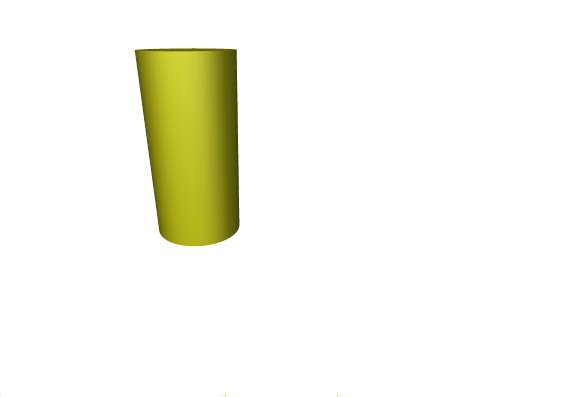
\includegraphics[width=\textwidth]{Plantilla-TFG-master/img/afin_trans.png}
        \caption{Traslación}
    \end{subfigure}
    \hfill
    \begin{subfigure}[b]{0.24\textwidth}
        \centering
        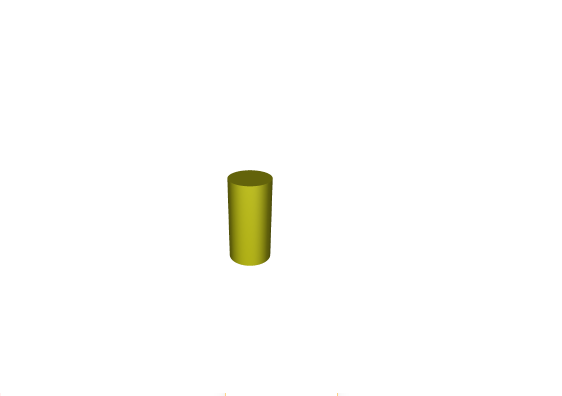
\includegraphics[width=\textwidth]{Plantilla-TFG-master/img/afin_scale.png}
        \caption{Escalado uniforme}
    \end{subfigure}
    \hfill
    \begin{subfigure}[b]{0.24\textwidth}
        \centering
        
\includegraphics[width=\textwidth]{Plantilla-TFG-master/img/afin_rot.png}
        \caption{Rotación}
    \end{subfigure}
    \hfill
   
    \caption{Ejemplos de uso de los operadores afines}
\end{figure}

\subsection{Operaciones deformantes}
Siguiendo el mismo razonamiento, podemos definir operaciones que modifiquen la geometría de la superficie aplicando rotaciones o traslaciones al punto en el que se evalúa la función distancia con signo original. De esta forma podemos obtener operadores que de otra forma sería mucho más complicado implementar, como la torsión o el redondeo de los bordes de una primitiva \cite{deform}.

\begin{definicion}[Operaciones Deformantes]
    Sea $A$ una isosuperficie. La función $\mu$ define la isosuperficie para las siguientes operaciones.
    \begin{itemize}
        
        \item \textbf{Torsión: } $\mu_{torsion}(p) = \sdf_{A}(p')$, con $p' = R_z(ky)\cdot (x,z,y)^t$.
        \item \textbf{Plegado: } $\mu_{plegado} =\sdf_{A}(p')$, con $p' = R_z(kx)\cdot p^t$.
        \item \textbf{Redondeo: } $\mu_{redondeo}(p) = \sdf_{A}(p) - k$.
        \item \textbf{Desplazamiento: } $\mu_{desplazamiento}(p) = \sdf_{A}(\delta(p))$.
        \item \textbf{Elongación de tamaño $\boldsymbol{h\in \R^3}$: } $\sdf_{elongacion}(p) = \mu_{A}(p')$, con $p' = p - c(p, -h, h)$.
    \end{itemize}
    En estas definiciones,
    \begin{itemize}
        \item $k\in \R^+_0$ controla la intensidad de la deformación,
        \item $\delta\colon \R^3\to \R^3$ es un patrón de desplazamiento,
        \item $R_z(\alpha)\in \mathcal{M}_3(\R)$ es la matriz de rotación de ángulo $\alpha$ sobre el eje $z$ dada en la \autoref{d:afines},
        \item $c\colon \R^3\times \R^3 \times \R^3 \to \R^3,\ c(x,a,b)$ acota cada componente de $x$ entre las de $a$ y $b$.
    \end{itemize}
\end{definicion}

Las únicas operaciones que nos proporcionan una función distancia con signo como resultado son el redondeo y la elongación. El resto es recomendable usarlas lo menos posible, pues las isosuperficies que generan pueden presentar fallos al ser renderizadas.
\begin{figure}[ht!]
    \centering
    \begin{subfigure}[b]{0.30\textwidth}
        \centering
        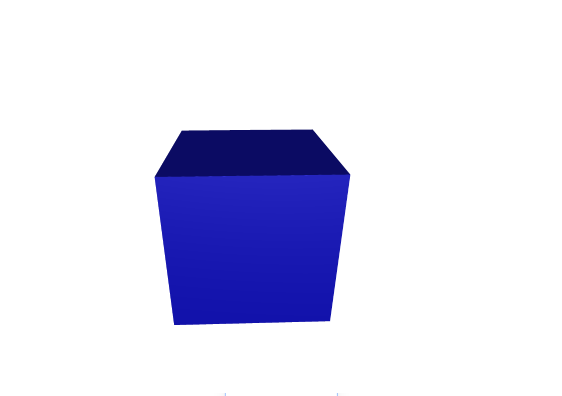
\includegraphics[width=\textwidth]{Plantilla-TFG-master/img/deform_og.png}
        \caption{Original}
    \end{subfigure}
    \hfill
    \begin{subfigure}[b]{0.30\textwidth}
        \centering
        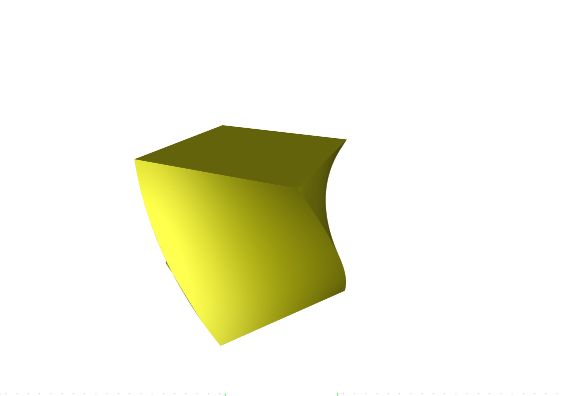
\includegraphics[width=\textwidth]{Plantilla-TFG-master/img/deform_twist.png}
        \caption{Torsión}
    \end{subfigure}
    \hfill
    \begin{subfigure}[b]{0.30\textwidth}
        \centering
        
\includegraphics[width=\textwidth]{Plantilla-TFG-master/img/deform_bend.png}
        \caption{Plegado}
    \end{subfigure}
    \hfill
    \begin{subfigure}[b]{0.30\textwidth}
        \centering
        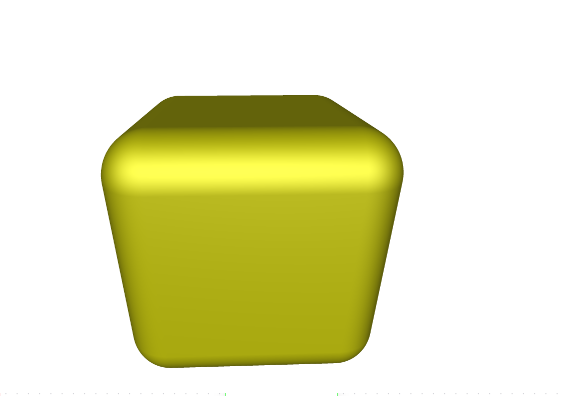
\includegraphics[width=\textwidth]{Plantilla-TFG-master/img/deform_round.png}
        \caption{Redondeo}
    \end{subfigure}
    \hfill
    \begin{subfigure}[b]{0.30\textwidth}
        \centering
        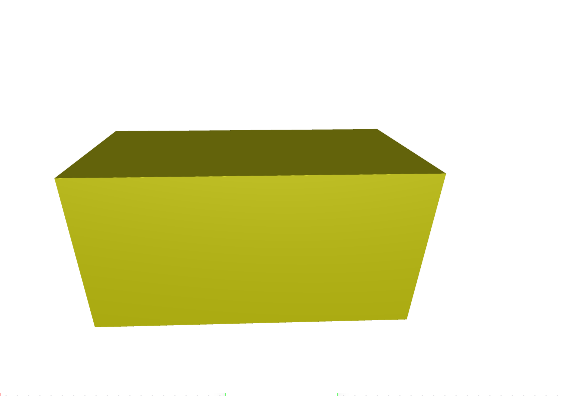
\includegraphics[width=\textwidth]{Plantilla-TFG-master/img/deform_elong.png}
        \caption{Elongación}
    \end{subfigure}
    
    \caption{Ejemplos de uso de los operadores de deformación}
\end{figure}

\subsection{Operaciones de repetición}
También podemos usar la técnica de cambiar el punto en el que evaluamos la función distancia para, en lugar de modificar la geometría original, añadir copias de la primitiva identificando varios puntos con uno que pertenezca a la isosuperficie. La manera más inmediata de conseguir esto es a través de la función valor absoluto, que nos permitirá identificar la componente de cada punto con su opuesta para generar simetrías, y el operador módulo, que identificará puntos a una distancia fija en cada eje.

\begin{definicion}[Operadores de Posicionamiento]\label{d:posicionamiento}
    Sea $A$ una isosuperficie. La función $\mu$ define la isosuperficie para las siguientes operaciones.
    \begin{itemize}
        \item \textbf{Simetrías sobre los ejes $\boldsymbol{x,y,z}$:}
        \begin{gather*}
            \mu_{simX}(p) = \sdf_{A}(\vert x\vert, y, z),\quad \mu_{simY}(p) = \sdf_{A}(x, \vert y\vert,  z),\\[5pt] \mu_{simZ}(p) = \sdf_{A}(x,y,\vert z\vert).
        \end{gather*}
        \item \textbf{Simetrías sobre los planos $\boldsymbol{xy,xz,yz}$:}
        \begin{gather*}
            \mu_{simXY}(p) = \sdf_{A}(\vert x\vert, \vert y\vert, z),\quad \mu_{simXZ}(p) = \sdf_{A}(\vert x\vert, y,  \vert z\vert),\\[5pt]\mu_{simYZ}(p) = \sdf_{A}(x,\vert y\vert ,\vert z\vert).
        \end{gather*}
        \item \textbf{Repetición $\boldsymbol{l\in \N^3}$ veces en los ejes $\boldsymbol{x,y,z}$ con separación $\boldsymbol{s\in\R}$:} 
        \begin{equation*}
            \mu_{rep}(p) = \sdf_{A}(p - s\cdot c\left(r\left(\frac{p}{s}\right), -l, l\right).
        \end{equation*}
        \item \textbf{Repetición infinita:}
        \begin{equation*}
            \mu_{repInf}(p) = \sdf_{A}\left((p+\frac{l}{2}\mod l )- \frac{l}{2}\right).
        \end{equation*}
    \end{itemize}
    En estas definiciones,
    \begin{itemize}
        \item $c\colon \R\times\R\times\R\to \R,\ c(x,a,b) = \Min(\Max(x, a), b)$ acota $x$ en $[a,b]$,
        \item $r\colon \R^3 \to \R^3$ redondea las componentes de un vector a sus enteros más cercanos.
    \end{itemize}
\end{definicion}
\begin{figure}[ht!]
    \centering
    \begin{subfigure}[b]{0.48\textwidth}
        \centering
        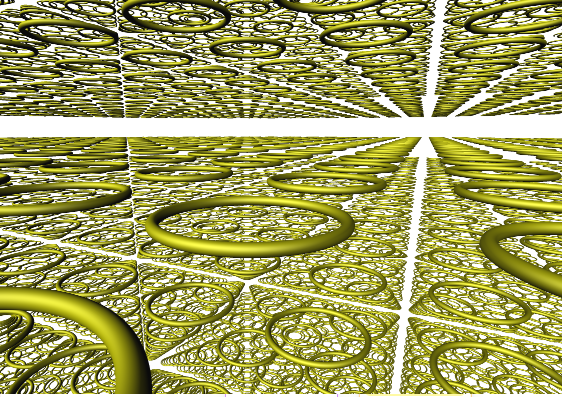
\includegraphics[width=\textwidth]{Plantilla-TFG-master/img/rep.png}
        \caption{Repetición infinita}
    \end{subfigure}
    \hfill
    \begin{subfigure}[b]{0.48\textwidth}
        \centering
        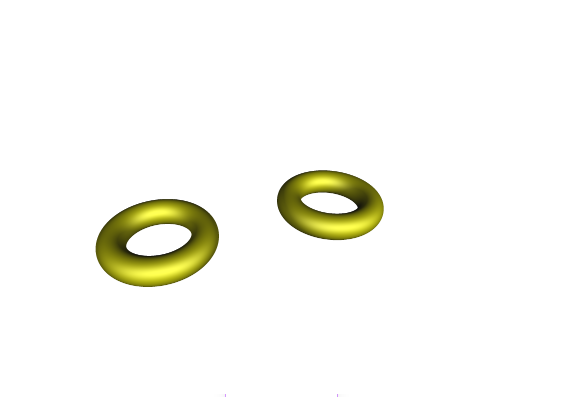
\includegraphics[width=\textwidth]{Plantilla-TFG-master/img/sym.png}
        \caption{Simetría}
    \end{subfigure}
    \hfill
        
    \caption{Ejemplos de uso de los operadores de repetición}
\end{figure}

Las funciones obtenidas no son en general funciones distancia con signo. Esto ocurre en los siguientes casos.
\begin{itemize}
    \item Al aplicar simetrías, cuando el objeto interseca el plano de simetría.
    \item En el caso de la repetición infinita, cuando las dimensiones del objeto sean mayores o iguales a $l/2$.
    \item Siempre para la repetición finita, como consecuencia de usar la función máximo. 
\end{itemize}

No obstante, este tipo de operaciones evidencia el potencial que tienen las funciones distancia con signo en cuanto a eficiencia a la hora de generar nuevas superficies, ya que podemos visualizar miles de objetos al precio de uno. Por ejemplo, podríamos generar un campo de césped a partir de una única brizna de hierba, o modelar solo una fracción de un objeto y generar el resto usando simetrías.



\section{Obtención a partir de ecuación implícita}
Empezábamos el capítulo diciendo que una de las representaciones más comunes de una superficie es a través de implícitas, pero hasta ahora nos hemos centrado en estudiar un subconjunto de esta familia. Si intentásemos aplicar el algoritmo de \textit{raymarching} a una función implícita cualquiera podríamos observar que el resultado presenta defectos, tales como deformaciones o grietas, o que incluso no se visualiza. Veamos qué podemos hacer para, dada una función implícita $\phi$ cualquiera, obtener información aproximada de $S_\phi$ \cite{article:aprox}. Esto nos será útil cuando no conozcamos o no podamos calcular explícitamente la función distancia con signo de una superficie, pero sí su ecuación implícita.

\begin{proposicion}
    Sea $\phi\colon \R^3\to\R$ una función implícita cualquiera. Entonces
    \begin{equation*}    
        \vert \sdf_{S_\phi}(p)\vert \le \frac{\vert \phi(p)\vert}{\Vert \nabla\phi(p)\Vert}.
    \end{equation*}
\end{proposicion}
\begin{proof}
    Fijamos el punto $p$ del cual queremos aproximar la distancia a $S_{\phi}$. Sea $q$ el punto de $S_\phi$ más cercano a $p$ y $v=\vec{pq}$. Queremos calcular la distancia de $p$ a $S_\phi$, que será justamente $\Vert v\Vert$. Asumiendo que $\phi$ es diferenciable en $p$, podemos realizar el desarrollo de Taylor de $\phi$ centrado en $p$:
    \begin{equation*}
        \phi(p) = \phi(p) + \nabla(p)\cdot (p+v -p) + \mathcal{O}(\vert p+v-p)\vert^2) = \phi(p) + \nabla(p)\cdot v + \mathcal{O}(\vert v\vert^2).
    \end{equation*}

    Suponemos ahora que $p$ está cerca de $S_\phi$, luego existe un $\varepsilon>0$ tal que  $\vert v\vert < \varepsilon$, y podemos obviar el residuo y $\phi(p)\approx \phi(q) = \phi(p+v)$. Como $\phi(q)=0$, tenemos que
    \begin{equation*}
        0 = \vert \phi(p+v)\vert \le \vert \phi(p) + \nabla(p)\cdot v \vert \le \vert \phi(p)\vert - \vert \nabla(p)\cdot v \vert         \le \vert \phi(p)\vert - \Vert \nabla(p)\Vert\cdot \Vert v \Vert,
    \end{equation*}
    donde hemos usado la desigualdad triangular y la linealidad del producto escalar. De esta expresión, finalmente deducimos que
    \begin{equation*}
        \Vert v\Vert \le \frac{\vert \phi(p)\vert}{\Vert \nabla(p)\Vert}.\qedhere
    \end{equation*}
\end{proof}
\begin{corolario}
    Sea $\phi\colon \R^3\to \R$ lipschitziana con constante $L$. Entonces
    \begin{equation*}    
        \vert \sdf_{S_\phi}(p)\vert \le \frac{\vert \phi(p)\vert}{\vert L\vert}.
    \end{equation*}
\end{corolario}

Este resultado solo nos proporciona una cota superior de la función distancia (sin signo). En nuestro caso esto es suficiente, pues esta nos sigue permitiendo representar la frontera de $S_{\phi}$. En su artículo \cite{art:impSdf}, Pierre-Alain Fayolle describe un método para obtener un SDF asociado a una superficie implícita que representa de manera exacta su frontera. Para ello descompone el SDF como 
\begin{equation*}
    sdf_{S_{\phi}}(p;\theta) = \phi(p)g(p;\theta)\quad \text{ o }\quad sdf_{S_{\phi}}(p;\theta) = sign(\phi(p))g(p;\theta),
\end{equation*}

donde $g$ es una función paramétrica de parámetros $\theta$ y $sign$ es una versión suavizada de la función signo, por ejemplo $sign(x) = \tanh{(kx)}$ con $k\in\R$. Para obtener la expresión de $g$ introduce la función implícita $\phi$ en la capa final de una red neuronal entrenada para  minimizar una función pérdida asociada al SDF, y para ajustar $\theta$ expresa $sdf_{S_{\phi}}(p;\theta)$ como la solución de un problema variacional. No obstante, esta técnica está fuera del ámbito de este trabajo, de forma que nos limitaremos a obtener la cota de la función distancia.

\section{Obtención a partir de ecuaciones paramétricas}

Ahora que sabemos representar las superficies generadas por una ecuación implícita cualquiera, nos proponemos ser capaces de representar también superficies definidas paramétricamente. Para ello fijaremos un anillo conmutativo $A$ y un conjunto de variables distintas $X=\{x_1,\dots, x_n\}$. Nuestro objetivo será, dado un conjunto $V\subseteq A^n$ por las ecuaciones paramétricas
\begin{align*}
    x_1 &= g_1(t_1,\dots, t_r),\\
    &\vdots \\
    x_n &= g_n(t_1,\dots, t_r),
\end{align*}
donde $g_i$ son polinomios de varias variables en $A$, obtener una ecuación implícita para $V$. En el caso que nos atañe $A=\R^3$, pero presentaremos todos los resultados de forma general.\newline

El contenido de esta sección está fuertemente basado en el libro Ideals, Varieties, and Algorithms de Cox, Little y O'Shea \cite{ideals_varieties}, el cual introduce de forma bastante completa resultados y algoritmos de álgebra conmutativa. Empezaremos explicando a qué nos referimos con polinomios de varias variables y recordando el concepto de ideal y sus propiedades. Después veremos que este problema equivale a uno de pertenencia a un ideal y cómo resolverlo usando la teoría de bases de Groebner.

\subsection{Polinomios en varias variables}
Estamos acostumbrados a trabajar con polinomios de una única variable como una suma o colección de monomios. Podemos mantener esta filosofía en el caso de varias variables adaptando el concepto que tenemos de estos.

\begin{definicion}
    Llamamos \textbf{monomio} en $X$ al producto de la forma
    $$x_1^{\alpha_1} \cdots x_n^{\alpha_n}\quad,\ \alpha_i \in \N,\ i\in\{1,\dots, n\}.$$
    Lo denotaremos como $X^{\alpha}$, y diremos que $\alpha\in \N^n$ es el \textbf{exponente} del monomio.
\end{definicion}

\begin{definicion}
    Definimos el \textbf{polinomio} $f:A^n\to A$ en $X$ con coeficientes en $A$ a toda combinación lineal finita de monomios
    \begin{align*}
        f = \sum_{\alpha\in \N^n} a_{\alpha} X^{\alpha}.
    \end{align*}

\end{definicion}

\begin{proposicion}
    El conjunto de polinomios es un anillo conmutativo. En concreto, para
     $$ f = \sum_{\alpha\in \N^n} a_{\alpha} X^{\alpha}\quad \text{ y }\quad g = \sum_{\beta\in \N^n} a_{\beta} X^{\beta},$$ 
     las operaciones internas del anillo son las siguientes.
    \begin{itemize}
        \item Suma heredada de $A$: $(f+g)(a) = f(a) + g(a)$.
        \item Producto de convolución: $(fg)(a) = \sum_{\alpha} \sum_{\beta+\gamma=\alpha} f(a)g(a)$.
    \end{itemize}
    Denotaremos como  $A[X] = A[x_1,\dots, x_n]$ a este anillo.
\end{proposicion}

En las siguientes secciones veremos que el problema de pertenencia de polinomios a un ideal se puede resolver mediante el procedimiento de la división. Este es bien conocido en polinomios de una variable, y ahora queremos extenderlo a un número arbitrario de ellas y varios divisores. Para ello en primer lugar necesitaremos una forma de ordenar los monomios que forman un polinomio. En una variable la forma \qq{natural} de comparar dos monomios es a través de su exponente. En el caso de varias variables la elección no es tan clara, y hay varias opciones que parecen igual de válidas. Vamos a formalizar el concepto de orden para introducir algunas de las posibilidades de las que disponemos. 

\begin{definicion}
    Un \textbf{orden total} sobre un conjunto $\Delta$ es una relación binaria $\le$ que cumple las siguientes propiedades.
    \begin{enumerate}
        \item Reflexiva: $a\le a,\ \text{para todo } a\in \Delta$.
        \item Transitiva: si $a\le b$ y $b\le c$ entonces $a\le c,\ \text{para todo } a,b,c\in \Delta$.
        \item Antisimétrica: si $a\le b$ y $b\le a$ entonces $a\le b,\ \text{para todo } a,b\in \Delta$.
        \item Completitud: $a\le b$ o $b\le a,\ \text{para todo } a,b\in \Delta$.
    \end{enumerate}
\end{definicion}
\begin{definicion}
    Un \textbf{orden admisible} es un orden total $\le$ sobre $\N^n$ cumpliendo
    \begin{enumerate}
        \item $(0,\dots ,0) \le \alpha,\ \text{para todo } \alpha \in \N^n$,
        \item si $\alpha < \beta$ entonces $\alpha + \gamma < \beta + \gamma,\ \text{para todo } \alpha,\beta,\gamma \in \N^n$.
    \end{enumerate}
\end{definicion}
\begin{proposicion}
    Todo orden admisible es un buen orden, esto es, todo subconjunto no vacío tiene un elemento mínimo.
\end{proposicion}

A partir de ahora siempre supondremos que todo orden que usemos es admisible en $\N^n$, luego podemos ordenar los monomios que conforman un polinomio ordenando sus exponentes según dicho orden. Veamos algunos de los órdenes más usados. 

\begin{definicion}
    Definimos el \textbf{orden lexicográfico} $\le_{\text{lex}}$ como
    \begin{equation*}
        \alpha \lex \beta \iff \begin{cases}
            \alpha  = \beta \\
            \quad\text{ó}   \\
            \alpha_i < \beta_i \text{, donde $i$ es el primer índice tal que } \alpha_i \neq \beta_i.
        \end{cases}
    \end{equation*}
\end{definicion}

% \begin{proof}
%     Es inmediato que es total, ya que $\le$ en $\N$ lo es. Veamos las otras condiciones.
%     \begin{enumerate}
%         \item Tomamos $\alpha \in \N^n$ tal que $\alpha\neq (0,\dots,0)$ y sea $i$ el primer índice tal que $\alpha_i \neq 0$. Entonces $0< \alpha_i$, de donde $(0,\dots, 0) \lex \alpha$.
%         \item Sean $\alpha$ y $\beta$ tales que $\alpha\lex \beta$, e $i$ el primer índice tal que $\alpha_i < \beta_i$
%     \end{enumerate}
% \end{proof}

\begin{definicion}
    Dado $\omega\in \N^n$, un orden admisible $\le$ se dice \textbf{$\boldsymbol{\omega}$-graduado} cuando
    \begin{equation*}
        \alpha\le \beta \text { implica que } \langle \alpha, \omega\rangle  < \langle \beta, \omega\rangle,
    \end{equation*}
    donde $\langle \alpha, \omega\rangle$ se llama el \textbf{$\boldsymbol{w}$-grado} de $\alpha$ y se define como
    \begin{equation}
        \langle \alpha, \omega\rangle = \alpha_1 \omega_1 + \cdots + \alpha_n \omega_n.
    \end{equation}
\end{definicion}

\begin{definicion}
    Dado un orden admisible $\le$, definimos el \textbf{orden $\boldsymbol{\omega}$-graduado asociado} como
    \begin{equation*}
        \alpha \le_{\omega} \beta \iff \begin{cases}
            \langle \alpha, \omega\rangle  < \langle \beta, \omega\rangle \\
            \quad\text{ó}   \\
           \langle \alpha, \omega\rangle = \langle \beta, \omega\rangle \text{ y } \alpha \le \beta.
        \end{cases}
    \end{equation*}
    Cuando $\omega = (1,\dots, 1)$ simplemente diremos que el orden es graduado, y usaremos las notaciones
    \begin{equation*}
        \le_{(1,\dots,1)} = \le_{\text{deg}},\quad (\lex)_{\text{deg}} = \le_{\text{deglex}},\quad (\lex)_{\omega} = \le_{\omega\text{-lex}}.
    \end{equation*}
\end{definicion}

\begin{definicion}
    Definimos el \textbf{orden lexicográfico graduado inverso} $\le_{\text{degrevlex}}$ como
    \begin{equation*}
        \alpha \le_{\text{degrevlex}} \beta \iff \begin{cases}
            |\alpha| < |\beta| \\
            \quad\text{ó}   \\
            |\alpha| = |\beta| \text{ y } \alpha_i > \beta_i \text{, donde $i$ es el último índice tal que } \alpha_i \neq \beta_i.
        \end{cases}
    \end{equation*}
\end{definicion}

\begin{proposicion}
    Sea $\le$ un orden admisible. Entonces $\le_{\omega}$ es admisible.
\end{proposicion}
\begin{proposicion}
    Los órdenes $\lex$ y $\le_{\text{degrevlex}}$ son admisibles.
\end{proposicion}

Una vez obtenida la noción de orden admisible, estamos en disposición de definir varios conceptos que nos resultarán imprescindibles para la manipulación de polinomios multivariable.

\begin{definicion}
    Sea $f= \sum_{\alpha} a_{\alpha} X^{\alpha}$ un polinomio y $\le$ un orden admisible. Definimos los siguientes conceptos asociados a $f$.
    \begin{itemize}
        \item \textbf{Exponente:} $exp(f) = \Max_{\le}(\alpha)$.
        \item \textbf{Monomio líder:}  $\lmf = X^{\expf}$.
        \item \textbf{Coeficiente líder:} $\lcf = a_{\expf}$.
        \item \textbf{Término líder:} $\ltf = \lcf \cdot \lmf$.
    \end{itemize}
\end{definicion}

\begin{definicion}
    Dado un monomio $X^{\alpha}$, definimos su \textbf{grado} como $\vert \alpha\vert = \alpha_1+\cdots + \alpha_n$. En el caso de un polinomio $f\in A[X]$, diremos que su grado es el grado de su monomio líder, y lo notaremos como $\deg(f)$.
\end{definicion}

Antes de presentar el algoritmo de la división, nos cercioramos de que esta operación siempre tiene sentido con el siguiente teorema.
\begin{teorema}[Algoritmo de división]
    Sea $F=\{f_1,\dots, f_s\} \subset A[X]$. Todo polinomio $f\in A[X]$ se puede expresar como
    \begin{equation*}
        f = q_1f_1 + \cdots + q_sf_s + r,
    \end{equation*}
    donde $q_i, r\in A[X]$ y $r=0$ ó $exp(r)\le exp(f)$. Llamaremos a $r$ el resto de dividir $f$ por $F$, y lo notaremos $\rem(f, [F]) = r$. Además, cuando $r=0$ diremos que $f$ reduce a $0$, y escribiremos $f \stackrel{F}{\to} 0$.
\end{teorema}

En otras palabras, podemos dividir $f$ entre cualquier conjunto de polinomios $F=\{f_1, \dots, f_s\}$ para expresarlo como combinación de sus elementos multiplicados por ciertos coeficientes polinómicos. El método es similar al usado en una variable, consistente en intentar reducir el monomio líder de $f$ restándole un múltiplo de cierto $f_i$. Para encontrar este $f_i$ simplemente se recorre el conjunto $F$ hasta encontrar uno válido, y de no haberlo se pasa el término líder al resto y se continua con el siguiente. Esto es justo lo que hace el \autoref{a:division}. Cabe destacar que esta forma de buscar el $f_i$ hace que la descomposición de $f$ obtenida no sea única, pues la elección dependerá de la posición que ocupen los divisores en el conjunto $F$, y por tanto del orden elegido. Más adelante veremos que la elección del orden influye en el resultado de más algoritmos.

\SetKwComment{Comment}{/* }{ */}
\begin{algorithm}[hbt!]
    \caption{División de polinomios en varias variables}\label{a:division}
    \KwData{dividendo $f$, divisores $F = \left[ f_1, \dots, f_s\right]$}
    \KwResult{Tupla con el resto $r$ y los coeficientes $q_i$ para cada $f_i\in F$}
    $p\gets f$
    
    $\left[q_1,\dots, q_s\right] \gets \left[0,\dots, 0\right]$
    
    $r\gets 0$

    \While{$p \neq 0$}{
        $\text{divisorEncontrado} \gets false$
        \For{$f_i \in F$} {
            \If{$\text{exp}(p) = \text{exp}(f_i) + \alpha$}{
                $q_i\gets q_i + \frac{\text{lc}(p)}{\text{lc}(f_i)} X^{\alpha}$
                
                $p \gets p - f_i \cdot \frac{\text{lc}(p)}{\text{lc}(f_i)} X^{\alpha}$
                
                $\text{divisorEncontrado} \gets true$
            }
        }
        \If{$!\text{divisorEncontrado}$}{
            $r \gets r + \text{lt}(p)$
            
            $p \gets p - \text{lt}(p)$
        }
    }
    \Return{$\left[r,q_1,\dots, q_s\right]$}
\end{algorithm}

\subsection{Bases de Groebner}
Ya tenemos claras las ideas sobre qué es un polinomio en varias variables, así que ahora pasamos a repasar el concepto de ideal y cómo podemos usar las bases de Groebner para trabajar con ellos en el caso de ideales de polinomios.
\begin{definicion}
    Decimos que $\emptyset \neq I \subseteq A[X]$ es un \textbf{ideal} de $A[X]$ si
    \begin{enumerate}
        \item $0\in I$,
        \item $a+b\in I,\ \text{para todo } a,b\in I$,
        \item $af\in I,\ \text{para todo } a\in I,\ \text{para todo } f\in A[x]$.
    \end{enumerate}
    En ese caso escribiremos $I\le A$.
\end{definicion}

\begin{proposicion}
    Dados los ideales $I,J\le A[X]$, son también ideales de $A[X]$:
    \begin{enumerate}
        \item $I+J = \{f+g : f\in I, g\in J\}$,
        \item $IJ = \{f_1g_1 + \cdots + f_tg_t : f_i\in I, g_i\in J, 1\le i \le t\}$,
        \item $I\cap J = \{h: h\in I \text{ y } h\in J\}$.
    \end{enumerate}
\end{proposicion}

Podemos calcular estos ideales usando sus conjuntos de generadores.
\begin{definicion}
    Dado $F=\{f_1,\dots, f_s\}\subseteq A[X]$, el \textbf{ideal generado} por $F$ es
    \begin{equation*}
        \langle F \rangle = \{a_1f_1 + \cdots + a_sf_s : a_1,\dots, a_s\in A,\ f_1,\dots, f_s\in F\}\le A[X].
    \end{equation*}
    Diremos que $F$ es un \textbf{conjunto de generadores} de $I$.
\end{definicion}

\begin{proposicion}
    Sean $I=\langle F\rangle$ y $J=\langle G\rangle$ ideales de $A[X]$. Entonces
    \begin{enumerate}
        \item $I+J = \langle F\cup G\rangle$,
        \item $IJ = \langle fg : f\in F, g\in G \rangle$,
        \item $I\cap J = \langle tF, (1-t)G \rangle \cap A[x_1,\dots, x_n]$.
    \end{enumerate}
\end{proposicion}

Pasamos a presentar el concepto de base de Groebner asociada a un ideal. Podemos pensar que una base de Groebner es a un ideal lo que un sistema de generadores a un espacio vectorial: un subconjunto a partir del cual podemos obtener el total.
\begin{definicion}
    Sea $I\le A[X]$. Denotamos el conjunto de los términos líder de $I$ como
    \begin{equation*}
        \lt(I) = \{\lt(f) : f\in I\}.
    \end{equation*}
\end{definicion}

\begin{definicion}
    Dado $I\le A[X]$, diremos que $G = \{g_1,\dots, g_s\}\subseteq I$ es una \textbf{base de Groebner} para $I$ si 
    $$\langle \lt(I)\rangle = \langle \lt(g_1),\dots, \lt(g_t) \rangle.$$
\end{definicion}

La analogía con el sistema de generadores de un espacio vectorial nos conduce de forma natural a la pregunta de si habrá también un análogo al concepto de base, y si dado un ideal $I$ siempre existirá una base de Groebner asociada a este. La respuesta es afirmativa en ambos casos.
\begin{definicion}
    Dada $f\in A[X]$, definimos su \textbf{soporte} como $$\supp(f) = \{ \alpha\in\Nn : f(\alpha) \neq 0\}.$$
\end{definicion}

\begin{definicion}
    Sea $I\le A[X]$. Diremos que $G$ es una \textbf{base de Groebner reducida} para $I$ si para todo $g\in G$ se cumple
    \begin{enumerate}
        \item $\lcg=1$,
        \item $\supp(g) \cap \left(\exp(G\setminus\{g\}) + \Nn \right) = \emptyset$.
    \end{enumerate}
    Es decir, una base será reducida si ningún elemento se puede expresar como combinación del resto. Esto equivale a que
    \begin{equation*}
        \rem\left(g, G\setminus \{g\}\right) \neq 0,\ \text{para todo } g\in G.
    \end{equation*}
\end{definicion}

\begin{definicion}
    Sea $M\le \Nn$. Decimos que $A$ es un \textbf{conjunto generador minimal} de $M$ si
    \begin{equation*}
        M = A + \Nn \quad \text{ y } \quad M\neq (A\setminus \{a\}) + \Nn,\ \text{para todo } a \in A.
    \end{equation*}
\end{definicion}

\begin{lema}\label{l:minimal}
    Todo ideal tiene un único conjunto generador minimal.
\end{lema}
\begin{lema}
    Sea $I\le A$. Se cumple que $a-b\in I,\ \text{para todo } a,b\in I$. 
\end{lema}
\begin{proof}\label{l:resta}
    Basta observar que tomando $-1 \in A$ obtenemos que $b\cdot (-1) \in I$, de donde
    \begin{equation*}
        a-b = a+ b(-1) \in I.\qedhere
    \end{equation*}
\end{proof}
\begin{teorema}\label{t:reduce}
    Todo ideal $I$ admite una única base de Groebner reducida para un orden admisible dado.
\end{teorema}
\begin{proof}
    \mybox{Existencia} Sea $G$ un conjunto generador minimal de $\exp(I)$, que sabemos que existe por el \autoref{l:minimal}. Sea $g\in G$ y $r = \rem\left(g, [G\setminus \{g\}]\right)$. Tenemos que
    \begin{equation*}
        \exp(g) \notin \exp(G\setminus\{g\}) + \Nn \text{ luego } \exp(g)=\exp(r),
    \end{equation*}
    de donde
    \begin{equation*}
        \exp(G) = \exp\Big( (G\setminus \{g\})\cup \{r\}\Big).
    \end{equation*}
    Además $g-r\in \langle G\setminus \{g\} \rangle \subseteq I$, de forma que $r\in I$ y $G' = (G\setminus \{g\} \cup \{r\}$ es una base de Groebner de $I$ cumpliendo $\supp(r) \cap \Big(\exp(G'\setminus\{r\}) + \Nn \Big) = \emptyset$.
    Aplicando este procedimiento a cada elemento de $G$ obtenemos una base reducida de $I$.\\[5pt]
    \mybox{Unicidad} Sean $G_1,G_2$ dos bases minimales de $I$. Por el \autoref{l:minimal}, como $\exp(G_1) = \exp(G_2)$, dado cualquier $g_1\in G_1$, no existe ningún $g_2\in G_2$ tal que $\exp(g_1) = \exp(g_2)$. Por otro lado, se cumple
    \begin{enumerate}
        \item $ \supp(g_1-g_2) \subseteq \Big( \supp(g_1)\cup \supp(g_2) \Big) \setminus \{\exp(g_1)\}$,
        \item $\supp(g_i)\setminus \{\exp(g_i)\}\cap \Big(\{\exp(G_i) + \Nn\}\Big) = \varnothing,\ i\in\{1,2\}$,
    \end{enumerate}
    de donde
    \begin{equation*}
        \supp(g_1-g_2) \cap \left(\exp(G_1)+\Nn\right) = \varnothing.
    \end{equation*}
    Concluimos entonces que $\rem(g_1-g_2, G_1) = g_1-g_2$, y como por el  \autoref{l:resta} sabemos que $g_2-g_1\in I$, dicho resto será igual a cero, de forma que $g_1=g_2$ y $G_1 = G_2$.
\end{proof}

Terminamos la sección obteniendo un algoritmo para calcular la base de Groebner reducida para un ideal dado un conjunto de generadores suyo $G$. Este se basará en eliminar de $G$ aquellos polinomios cuyos exponentes podamos poner como combinación lineal del resto. Claro está que no podemos realizar esta comprobación directamente, y deberemos buscar alguna condición equivalente que sí podamos calcular.

\begin{definicion}
    Dados $\alpha,\beta \in \Nn$, definimos los términos
    \begin{itemize}
        \item \textbf{Mínimo común múltiplo}: $\lcm(\alpha,\beta) = \{\Max(\alpha_1, \beta_1),\dots, \Max(\alpha_n, \beta_n)\}$,
        \item \textbf{Máximo común divisor}: $\gcd(\alpha,\beta) = \{\Min(\alpha_1, \beta_1),\dots, \Min(\alpha_n, \beta_n)\}$.
    \end{itemize}
\end{definicion}

\begin{definicion}
    Sean $f,g \in A[X]$. Tomando $\alpha=\exp(f),\ \beta=\exp(g)$ y $\gamma = \lcm(\alpha,\beta)$, se define el \textbf{S-polinomio} de $f$ y $g$ como
    \begin{equation*}
        S(f,g) = \lc(g)X^{\gamma-\alpha}f - \lc(f)X^{\gamma-\beta}g.
    \end{equation*}
\end{definicion}

\begin{teorema}[Primer Criterio de Buchberger]\label{t:criterio}
    Sean $I\le A[X]$ y $G=\{g_1,\dots, g_t\}$ un conjunto de generadores de $I$. Entonces:
    \begin{equation*}
        G \text{ es base de Groebner para } I \iff \rem(S(g_i,g_j), G)=0,\ \text{para todo } 1\le i<j\le t.
    \end{equation*}
\end{teorema}

El algoritmo que usaremos para el cálculo de la base de Groebner se basará en este criterio. Sin embargo, antes de presentarlo estudiamos dos criterios adicionales \cite{criterio1,criterio2} que lo harán más eficiente descartando S-polinomios antes de comprobar su resto, ahorrando el cómputo de numerosas divisiones.

\begin{definicion}
    Sea $f= \sum_{\alpha} a_{\alpha} X^{\alpha}$ un polinomio cuyo monomio líder es $X^{\alpha^{(k)}}$ y $\le$ un orden admisible. Definimos el \textbf{segundo monomio líder} de $f$ como el monomio $X^{\alpha^{(i)}}$ de $f$ tal que
    \begin{equation*}
        X^{\alpha^{(i)}} \ge X^{\alpha^{(j)}},\ \text{ para todo } j\notin\{i,k\}. 
    \end{equation*}
    Lo denotaremos como $\sm(f)$.
\end{definicion}
\begin{teorema}[Criterios de Buchberger]\label{t:criterios}
    Sean $I\le A[X]$, $G\subseteq A[X]$ un conjunto de generadores de $I$, y $g_1,g_2 \in G$. Si se cumple cualquiera de las siguientes condiciones entonces  $S(g_1,g_2)\reduces 0$.
    \begin{enumerate}
        \item $\lcm(g_1,g_2) = \lm(g_1)\lm(g_2)$,
        \item existe un $f\in G$ tal que $\lm(f)\ \vert\ \lcm(g_1,g_2)$ y además
        \begin{enumerate}
            \item algún $S(g_i,f)\reduces 0\quad$ ó
            \item $\lm(f)\vert \frac{\lm(g_i)}{\gcd(g_1,g_2}$ y $\sm(g_j)\lm(f) \neq \sm(f)\lm(g_j)$,
        \end{enumerate}
        donde $i,j\in\{1,2\}$ e $i\neq j$.
    \end{enumerate}
    
\end{teorema}

Usando los criterios obtenidos obtenemos el \autoref{a:buchberger} para calcular la base de Groebner de cualquier ideal. La salida de este no es una base minimal, pero la demostración del \autoref{t:reduce} nos proporciona un método para reducir una base cualquiera a la minimal asociada. En el \autoref{a:minim} mostramos este procedimiento.\newline

\SetKwComment{Comment}{/* }{ */}
\begin{algorithm}[hbt!]
    \caption{Algoritmo de Buchberger optimizado}\label{a:buchberger}
    \KwData{polinomio $f$, conjunto de generadores $F = \left[ f_1, \dots, f_S\right]$}
    \KwResult{base de Groebner $G$}

    $G\gets F$\;

    \Repeat{$G' = G$}{
        $G'\gets G$\;
        \For{each pair $\{f,g\} \subseteq G'$} {
            \If{$\text{!Criterio 1}(f,g) \textbf{ AND } !\text{Criterio 2}(f,g, G')$}{
                $r\gets \rem(S(f,g), G')$\;
                \If{$r\neq 0$}{
                    $G\gets G\cup \{r\}$\;
                }
            }
        }
    }

    \Return{$G$}
\end{algorithm}

\begin{algorithm}[hbt!]
    \caption{Minimización de base de Groebner}\label{a:minim}
    \KwData{$G$ base a minimizar}

    $G\gets F$\;

    \ForEach {$g \in G$}{
        $g\gets g/\lc(g)$\;
        $r\gets \rem(g, [G\setminus \{g\}])$\;

        \If{$r\neq 0$}{
            $g \gets r$\;
        }
    }
\end{algorithm}

Ya somos capaces de obtener una base de Groebner minimal de cualquier ideal dado un conjunto de generadores suyo, pero en este proceso se toma una decisión que aún no hemos discutido: cómo se eligen las parejas $\{f,g\}$. Uno de los métodos más usados es la conocida como \textbf{estrategia normal}, debido a su simpleza y haber probado ser de las que completan más rápido el algoritmo, y consiste en tomar el par $f,g$ cuyo $\lcm(f,g)$ sea del menor grado posible según el orden admisible usado. Vemos por tanto que de nuevo la elección de un orden u otro nos proporcionará resultados diferentes, y en este caso esto se traduce en que la base reducida tenga muchos menos elementos en un orden que en otro.

\subsection{Teorema de implicitación}
Empezábamos la sección diciendo que el problema de implicitación equivalía al de pertenencia a un ideal. Antes de ver de qué ideal se trata tenemos que introducir unos últimos conceptos que nos ayuden a entender por qué.

\begin{definicion}Dado $F=\{f_1,\dots, f_s\} \subseteq A[X]$, llamamos \textbf{variedad afín} definida por $F$ al conjunto:
    \begin{equation*}
        \mathbb{V}(F) = \{(a_1,\dots, a_n)\in A^n : f_i(a_1,\dots, a_n)=0,\ \text{para todo } i\in\{1,\dots, s\}\}.
    \end{equation*}
\end{definicion}

\begin{proposicion}
    Sean $\mathbb{V}(F)$ y $\mathbb{V}(G)$ variedades afines. Entonces
    \begin{itemize}
        \item  $\mathbb{V}(F) =  \mathbb{V}(\langle F\rangle)$,
        \item $\mathbb{V}(F\cup G) = \mathbb{V}(F) \cap \mathbb{V}(G)$,
        \item $\mathbb{V}(FG) = \mathbb{V}(F) \cup \mathbb{V}(G)$.
    \end{itemize}
\end{proposicion}

\begin{proposicion}
    Sean los ideales $I,J\le A[X]$. Entonces  $\mathbb{V}(I \cap J) = \mathbb{V}(I) \cup \mathbb{V}(J)$.
\end{proposicion}
\begin{definicion}
    Sea $B\subseteq A^n$. Definimos el \textbf{ideal asociado} a $B$ como
    \begin{equation*}
        \mathbb{I}(B) = \{f\in A[X] : f(b_1,\dots, b_n) = 0,\ \text{para todo } (b_1,\dots, b_n)\in B\}.
    \end{equation*}
\end{definicion}

Para resolver el problema de implicitación deberemos aprender antes a eliminar variables de un ideal.
\begin{definicion}
    Dado $I\le A[x_1,\dots,x_n]$, definimos su \textbf{ideal de $l$-eliminación} como
    \begin{equation*}
        I_l = I \cap A[x_{l+1}, \dots, x_n] \le A[x_{l+1}, \dots, x_n].
    \end{equation*}
\end{definicion}

\begin{definicion}
    Decimos que un orden admisible $\le$ es un \textbf{orden de $l$-eliminación} si 
    $$\beta\le \alpha \text{ implica } \beta \in \N_l^n,\ \text{para todo } \alpha \in \N_l^n \text{ y } \text{para todo } \beta \in \Nn,$$
    donde $\N_l^n = \{\alpha\in \Nn \colon \alpha_i =0,\ 1\le i \le l\}$.
\end{definicion}

\begin{teorema}[Eliminación]
    Sea $I\le A[x_1,\dots,x_n]$ y $G$ una base de Groebner suya respecto a un orden $\le$ de $l$-eliminación. Entonces, una base de Groebner para $I_l$ viene dada por
    \begin{equation*}
        G_l = G\cap A[x_{l+1},\dots, x_n].
    \end{equation*}
\end{teorema}

% Ahora sí, veamos de qué ideal se trata.

Con estos resultados podemos decir que el problema de implicitación consiste en encontrar la variedad asociada a las ecuaciones paramétricas
\begin{equation*}
    \begin{cases}
    x_1 &= g_1(t_1,\dots, t_r),\\
    &\vdots \label{eq:paramEq} \\
    x_n &= g_n(t_1,\dots, t_r).
    \end{cases}
\end{equation*}
Si escribimos $g_i = f_i/q_i$ con $f_i,q_i \in A[t_1,\dots, t_r]$ para $i=1,\dots, r$, podemos definir la aplicación
\begin{align*}
        \phi \colon A^r\setminus W  & \to A^n,\\
        (a_1,\dots, a_r) & \mapsto \left( \frac{f_1(a_1,\dots, a_r)}{q_1(a_1,\dots, a_r)}, \dots, \frac{f_n(a_1,\dots, a_r)}{q_n(a_1,\dots, a_r)}\right),
    \end{align*}
donde $W=\mathbb{V}(q_1\cdots q_r)$. Veamos cómo encontrar la menor variedad que contiene la imagen de $\phi$ en el caso de que $q_i = 1$ para cada $i\in \{1,\dots, r\}$. 
\begin{teorema}[Implicitación Polinomial]\label{t:implicit}
    Dados $f_1,\dots, f_n \in A[t_1, \dots, t_r]$ con $A$ cuerpo infinito, sea
    \begin{align*}
        \phi \colon A^r  & \to A^n,\\
        (a_1,\dots, a_r) & \mapsto \left( f_1(a_1,\dots, a_r), \dots, f_n(a_1,\dots, a_r) \right).
    \end{align*}
    Definimos los ideales:
    \begin{itemize}
        \item $I = \langle x_1-f_1,\dots,  x_n-f_n\rangle \le A[t_1,\dots, t_r,x_1\dots, x_n]$,
        \item $J = I\cap A[x_1,\dots, x_n]$ el ideal de $r$-eliminación de $I$.
    \end{itemize}
    Entonces, $\mathbb{V}(J)$ es la menor variedad que contiene a $\phi(A^r)$.
\end{teorema}


La extensión al caso racional es la siguiente.
\begin{teorema}[Implicitación Racional]\label{t:implicitRac}
    Sea $f_1,\dots, f_n, q_1,\dots, q_n \in A[t_1, \dots, t_r]$ con $A$ cuerpo infinito, $W=\mathbb{V}(q_1,\dots, q_n)$ y
    \begin{align*}
        \phi \colon A^r\setminus W  & \to A^n,\\
        (a_1,\dots, a_r) & \mapsto \left( \frac{f_1(a_1,\dots, a_r)}{q_1(a_1,\dots, a_r)}, \dots, \frac{f_n(a_1,\dots, a_r)}{q_n(a_1,\dots, a_r)}\right).
    \end{align*}
     Definimos los ideales:
    \begin{itemize}
        \item $I = \langle q_1x_1-f_1,\dots,  q_nx_n-f_n, 1-q_1\cdots q_ny\rangle \le A[y,t_1,\dots, t_r,x_1\dots, x_n]$,
        \item $J = I\cap A[x_1,\dots, x_n]$ el ideal de $1+r$-eliminación de $I$.
    \end{itemize}
    Entonces, $\mathbb{V}(J)$ es la menor variedad que contiene a $\phi(A^r\setminus W)$.
\end{teorema}

\begin{observacion}
    En el caso $r=1$ y cuando $f_i$ y $q_i$ sean primos relativos para cada $1\le i \le n$, basta tomar
    $$I = \langle q_1x_1-f_1,\dots,  q_nx_n-f_n\rangle.$$
\end{observacion}

Con este resultado, una vez obtenida la variedad, si resulta que esta tiene un único generador este será una potencia la ecuación implícita, luego el ideal al que llevamos haciendo referencia desde el principio de la sección y del que queríamos comprobar la pertenencia es el ideal $J$ de los teoremas anteriores. El hecho de que no obtengamos la potencia exacta de la ecuación implícita no es problema, pues nos basta conocer donde se anula para poder representar la frontera de la superficie que genera.  Sin embargo, no tenemos asegurado que vaya a haber un único generador del ideal, de forma que la superficie satisfaría varias ecuaciones implícitas y no podría ser representada por una sola. A continuación presentamos un resultado que aporta información al respecto.

\begin{definicion}
    Dado un ideal $I\le A[X]$, definimos su radical como
    \begin{equation*}
        \sqrt{I} = \{f\in A[X] : f^m\in I \text{ para algún } m\in \N\}.
    \end{equation*}
\end{definicion}
\begin{proposicion}
    Sea $I\le A[X]$. Entonces $\sqrt{I}$ es un ideal y contiene a $I$.
\end{proposicion}
\begin{definicion}
    Decimos que un ideal $I\le A[X]$ es \textbf{radical} si $\sqrt{I} = I$.
\end{definicion}

\begin{proposicion}
    Sea $B\subseteq A^n$. Entonces $\mathbb{I}(B)$ es un ideal radical.
\end{proposicion}
\begin{teorema}[Nullstellensatz fuerte]
    Si $A$ es algebraicamente cerrado, dado un ideal $I\le A[X]$ se cumple
    \begin{equation*}
        \sqrt{I} = \mathbb{I}(\mathbb{V}(I)).
    \end{equation*}
\end{teorema}
\begin{proposicion}
    Sea $I\le A[X]$ y $f\in A[X]$. Entonces
    \begin{equation*}
        f\in \sqrt{I} \text{ si y solo si } \langle I \rangle + \langle 1-fy \rangle = A[X].
    \end{equation*}
\end{proposicion}
Así, si pudiéramos calcular el radical del ideal $J$ de los teoremas de implicitación y este tuviera un solo elemento, tendríamos asegurado que la variedad está generada por esa única ecuación implícita. Además, calculando el radical podríamos obtener también la potencia exacta de la ecuación implícita que obtuvimos con el \autoref{t:implicitRac}. Sin embargo, el cálculo del radical o su número de elementos es en general muy complicado, y no es una opción viable. Por tanto, lo que haremos en la práctica será simplemente aplicar el algoritmo y comprobar si efectivamente se obtiene un único generador, en cuyo caso contrario concluiremos que no podemos realizar la implicitación.\newline

Hay otros métodos diferentes que permiten abordar el problema de eliminación de variables, y por tanto el de implicitación. Uno especialmente interesante es el uso de resultantes, pues en casos específicos puede simplificar mucho la obtención de la ecuación implícita. En la siguiente sección estudiaremos como podemos usar de forma básica el resultante del sistema de ecuaciones \eqref{eq:paramEq} para obtener su representación implícita.





\chapter{Algoritmos de visualización de SDFs}\label{cap:2}
Una vez estudiadas las técnicas a través de las cuales podemos crear y manipular primitivas, podemos usar estas para formar la escena que queremos representar. Podemos optar por dos enfoques. El primero de ellos es hacer \textit{spheretracing} una vez por cada primitiva que conforme la escena, lo cual permitiría tener un control más preciso sobre las propiedades de cada objeto de la escena de forma individual, como por ejemplo su apariencia (material) o distancia de dibujado. El otro enfoque consiste en combinar todas las primitivas de la escena en una sola mediante el operador booleano de unión. La principal ventaja en este caso sería el tener toda la escena definida a partir de una única SDF, de forma que tenemos la información más condensada y el renderizado es más sencillo al no tener que combinar el resultado de varias ejecuciones del algoritmo de \textit{spheretracing}. El precio a pagar por esta simplicidad es que perdemos el control más granular que sí teníamos antes. No obstante, optaremos por este último enfoque, tanto por simplicidad como porque nuestro objetivo final es crear nuevas superficies, y lo que más sentido tiene es que usemos una única SDF para representarlas.\newline

Ahora que tenemos definida la escena a partir de una función distancia con signo, necesitamos una forma de visualizarla. En IG se utilizan diferentes técnicas y algoritmos que transforman datos geométricos en otros que nuestras pantallas puedan representar. Dos de los métodos más utilizados son la rasterización y el trazado de rayos o \textit{raytracing}. En general, la rasterización es el método más usado para aplicaciones interactivas, ya que las GPUs fueron originalmente diseñadas para realizar rasterización de forma eficiente. Por otro lado, el \textit{raytracing} ofrece resultados más realistas, sobretodo en los aspectos relacionados con la iluminación, a precio de ser más lento. En los últimos años son cada vez más comunes las GPUs con soporte hardware para \textit{raytracing}, haciendo que se extienda su uso a aplicaciones interactivas, como los videojuegos.\newline

A la hora de trabajar con estos algoritmos es importante la forma en la que se representa la información de la geometría. La más común en rasterización y \textit{raytracing} es a través de mallas de polígonos, un conjunto de puntos de un espacio afín que forman caras planas. En ambos algoritmos necesitamos hacer uso del concepto de primitiva como los elementos más pequeños que pueden ser visualizados, y típicamente se trata de triángulos cuando se trabaja con mallas de polígonos. En nuestro caso no usamos mallas de polígonos, y tenemos una representación no discreta de la geometría de la superficie. Si bien la rasterización se puede adaptar para trabajar con objetos diferentes a mallas de polígonos, esto no es lo común, y el \textit{raytracing} es mucho más adaptable en estos casos, pues permite trabajar con cualquier tipo de objeto con el que se pueda calcular la intersección con un rayo, como ocurre con las SDFs.\newline

La \textbf{rasterización} recorre cada primitiva $P$ del modelo, comprobando para cada una qué conjunto $S$ de pixels de la pantalla la cubren. Una vez obtenidos los pixels, se ejecutará un programa escrito por el programador (\textit{fragment shader}) para cada uno de ellos, que calculará el color final del píxel. El funcionamiento del \textbf{\textit{raytracing}} es similar al de la rasterización, pero intercambiando los dos bucles. El procedimiento consiste por tanto en recorrer los pixels de la pantalla y comprobar qué primitivas del modelo cubren cada uno. Para ello se traza un rayo por el centro de cada píxel y se calcula la intersección con el objeto, razón del nombre \qq{trazado de rayos}. En la \autoref{fig:algVis} y la \autoref{fig:colorPixels} podemos apreciar las diferencias en el procedimiento de ambos algoritmos. Ambos métodos tienen complejidad algorítmica $\mathcal{O}(pn)$, siendo $n$ el número de primitivas y $p$ el de pixels, aunque en el caso del \textit{raytracing} esta se puede mejorar usando indexación espacial para la obtención del conjunto de primitivas que cubren cada píxel.\newline

\begin{figure}[ht!]
    \centering
    \begin{minipage}{0.47\textwidth}
        \begin{algorithm}[H]
            \caption{Rasterización}
            inicializar color de todos los pixels
            
            \For{cada primitiva $P$ en el modelo}{
                $S\gets $ pixels cubiertos por $P$

                \For{cada píxel $q$ en $S$}{
                    calcular color de $P$ en $q$

                    actualizar color de $q$
                }
            }
        \end{algorithm}
    \end{minipage}%
    \hfill
    \begin{minipage}{0.47\textwidth}
        \begin{algorithm}[H]
            \caption{\textit{Raytracing}}
            inicializar color de todos los pixels
            
            \For{cada píxel $q$ de la pantalla}{
                $T\gets $ primitivas que cubren $q$

                \For{cada primitiva $P$ en $T$}{
                    calcular color de $P$ en $q$

                    actualizar color de $q$
                }
            }
        \end{algorithm}
    \end{minipage}%
    \caption{Algoritmos de visualización}
    \label{fig:algVis}
\end{figure}

\begin{figure}[!ht]
     \begin{minipage}[c]{0.98\linewidth}
        \centering
        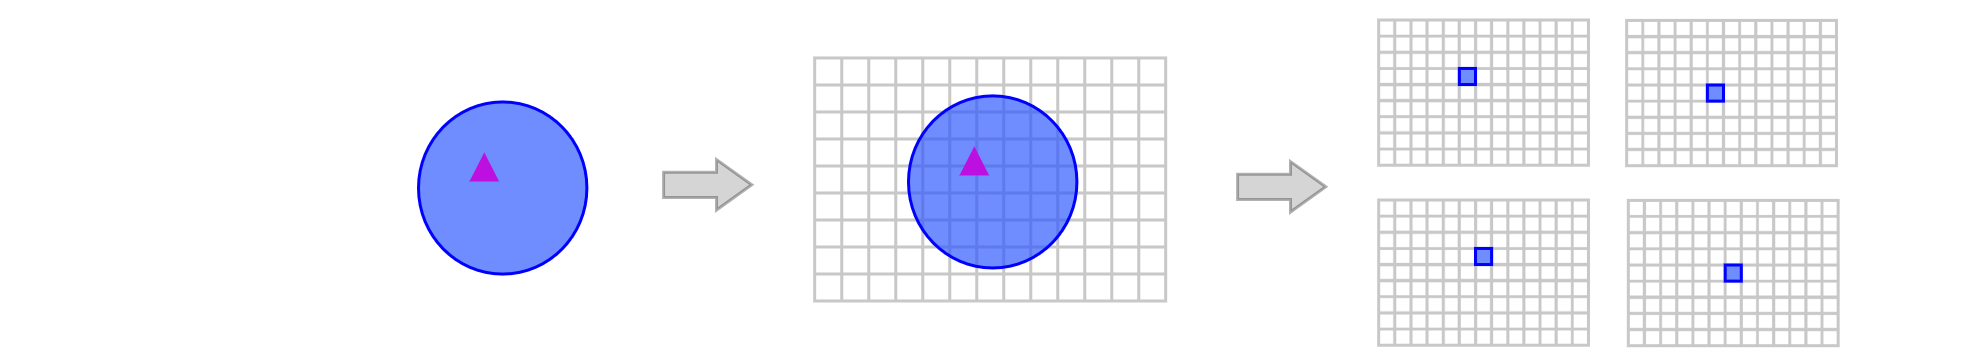
\includegraphics[width=0.9\textwidth]{Plantilla-TFG-master/img/rasterizacion.png}
        \caption{Rasterización}
     \end{minipage}
     \begin{minipage}[c]{0.98\linewidth}
        \centering
        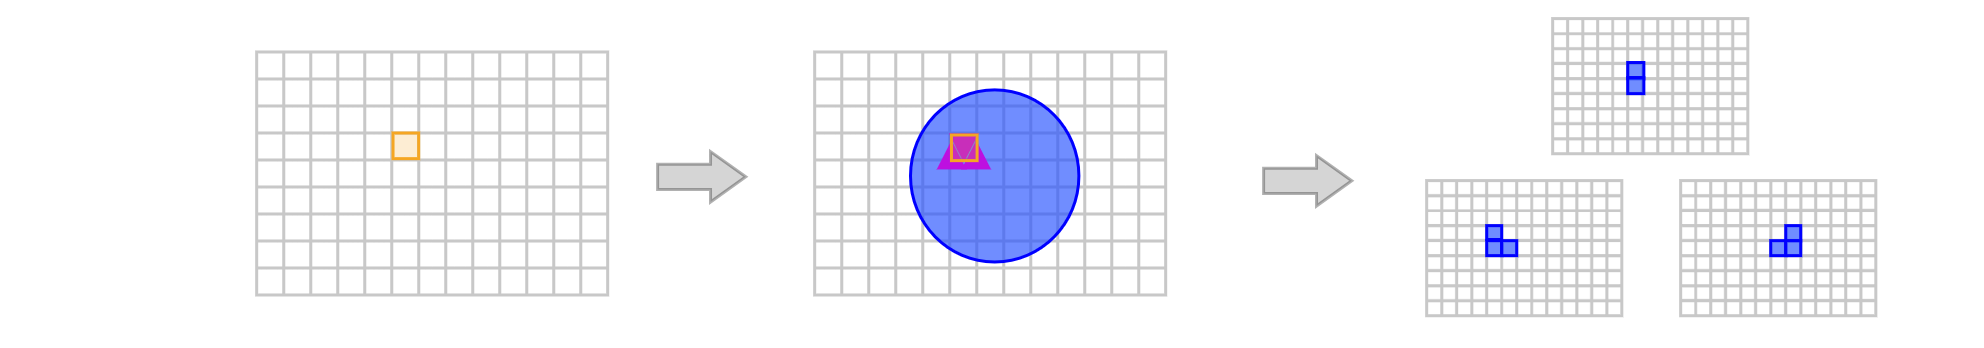
\includegraphics[width=0.9\textwidth]{Plantilla-TFG-master/img/raytracing.png}
        \caption{\textit{Raytracing}}
     \end{minipage}
     \caption{Funcionamiento de los métodos de rasterización y \textit{raytracing}}
     \label{fig:colorPixels}
\end{figure}

Teniendo en cuenta las consideraciones anteriores, para representar superficies generadas por funciones distancia con signo  utilizaremos \textit{spheretracing}, un método basado en \textit{raytracing}. No obstante, para ello haremos uso de las APIs de rasterización en GPU, lo cual puede parecer contradictorio, pues como hemos visto ambos algoritmos tienen una estructura opuesta. El motivo fundamental de esta aparente contradicción es que las APIs de \textit{raytracing} solo están disponibles en GPUs modernas y avanzadas, y nosotros queremos poder realizar esta tarea en el mayor número de dispositivos posible. Podríamos conseguir esto realizando los cálculos en la CPU recorriendo secuencialmente los pixels, pero incluso paralelizándolos en varias hebras asignando a cada una un conjunto de pixels no podríamos conseguir el grado de interactividad que buscamos. La única solución es por tanto usar la GPU para realizar los cálculos de la intersección rayo-escena, pues son mucho más rápidas en este tipo de cálculos. Además, hoy en día prácticamente todos los dispositivos cuentan con GPUs, incluso los dispositivos móviles, y las APIs de rasterización son muy portables y conocidas. \newline

Para lograr nuestro objetivo de trazar rayos usando las APIs de rasterización usaremos que, como hemos visto, estas permiten ejecutar para cada píxel donde se proyecte una primitiva un código definido por el programador llamado \textit{fragment shader} y que produce el color del píxel. Así, en lugar de hacer \textit{raytracing} sobre una escena 3D, visualizaremos por rasterización un plano formado por dos triángulos cubriendo toda la imagen, lo que provocará la ejecución de una instancia del \textit{fragment shader} en cada píxel de la imagen, y será en él donde se implemente el algoritmo de intersección rayo-escena. A este plano lo llamaremos \textbf{lienzo} o \textit{canvas}, pues efectivamente estaremos pintando la escena encima suya píxel a píxel a través del \textit{fragment shader}.

\section{Renderizado por \textit{raytracing} en GPU usando un \textit{fragment shader}}\label{sec:render}
En esta sección estudiaremos en detalle el proceso de creación del lienzo usando una API cualquiera de rasterización y el desarrollo de los cálculos necesarios para ello , incluyendo la intersección del rayo con la escena, simulación avanzada de iluminación y técnicas de suavizado de la imagen.
\subsection{Creación del lienzo}\label{sec:lienzo} 
Cuando introdujimos el método de rasterización dijimos que este suele ser usado con mallas de polígonos, que a su vez estaban compuestas por puntos en un espacio afín que se unen formando caras. Lo cierto es que en IG se hace uso de múltiples espacios de coordenadas, los cuales es imprescindible conocer para entender el proceso de definición de geometría y pasamos a enumerar.
% Si bien se puede hacer \textit{raymarching} directamente sobre una escena 3D, nuestra escena constará únicamente de un plano formado por cuatro vértices y dos triángulos, que usaremos como lienzo  (o \textit{canvas}) para dibujar sobre él. Para ello, necesitaremos trabajar sobre diferentes espacios de coordenadas que pasamos a enumerar.
\begin{itemize}
    \item \textbf{Coordenadas locales o de objeto:} distancias relativas al origen del objeto.
    \item \textbf{Coordenadas globales o de mundo:} distancias relativas a un origen común para todos los objetos.
    \item \textbf{Coordenadas de cámara:} distancias relativas a un sistema de referencia posicionado y alineado con la cámara.
    \item \textbf{Coordenadas de recortado:} distancias normalizadas en el rango $[-1,1]^2$ relativas a un sistema asociado al rectángulo que forma la imagen en pantalla.
    \item \textbf{Coordenadas de dispositivo:} están centradas en la esquina inferior izquierda de la pantalla y toman valor en el rango $[0,r_x]\times [0,r_y]$, donde $r=(r_x,r_y)$ es la resolución de la pantalla.
\end{itemize}

% Si hacemos uso de \texttt{GL\_TRIANGLES} bastará con definir los vértices en sentido antihorario, pero hay que tener en cuenta que tendremos que repetir dos vértices, ya que se irán formando los triángulos en grupos de tres vértices. Una alternativa para no repetir vértices sería utilizar tablas de vértices e índices, pero en nuestro caso no merece la pena al tener únicamente seis vértices. Un ejemplo de definición de vértices formando un lienzo rectangular podría ser el que se muestra en la \autoref{fig:canvas}.\newline

% \begin{figure}[ht]
%     \centering
%     \begin{minipage}{0.50\textwidth}
%         \begin{lstlisting}
% glBegin(GL_TRIANGLES);
%     glColor3f(1.0f, 1.0f, 1.0f); 
    
%     // Triangulo inferior
%     glVertex3f(-2.0f, -1.0f, 0.0f);
%     glVertex3f(-2.0f, 1.0f, 0.0f);
%     glVertex3f(2.0f, 1.0f, 0.0f);
    
%     // Triangulo superior
%     glVertex3f(-2.0f, -1.0f, 0.0f);
%     glVertex3f(2.0f, 1.0f, 0.0f);
%     glVertex3f(2.0f, -1.0f, 0.0f);
% glEnd();
% \end{lstlisting}
%     \end{minipage}%
%     \hfill
%     \begin{minipage}{0.40\textwidth}
%         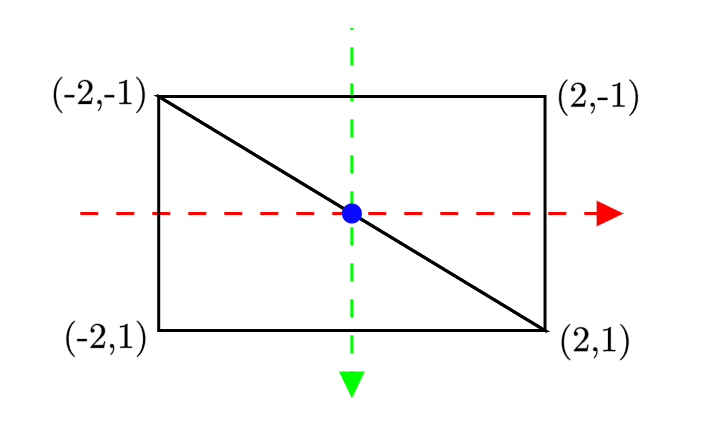
\includegraphics[width=\textwidth]{canvas.png}
%     \end{minipage}
    
    
%     \caption{Construcción del lienzo}
%     \label{fig:canvas}
% \end{figure}
Dado que para usar rasterización el lienzo deberá estar definido como una malla de polígonos, deberemos declarar los vértices que la conforman y cómo estos se unen formando primitivas, en este caso triángulos. Este lienzo, como toda geometría, tendrá asignado dos \textit{shaders} o procesadores, que son programas que se ejecutan en la GPU. Estos programas pueden recibir parámetros, pero son independientes entre sí, siendo la única forma en la que pueden comunicarse entre ellos mediante el paso de atributos de entrada y salida. Hay dos tipos de \textit{shaders}: de vértices (\textit{vertex shader}) y de fragmentos o pixels (\textit{fragment shader}), cada uno con atributos específicos de entrada y salida.\newline

En el \textit{vertex shader} utilizaremos los siguientes atributos.
\begin{itemize}
    \item $v_{loc}$: vector de cuatro flotantes que contiene las coordenadas
    homogéneas locales del vértice a procesar. La cuarta componente es la componente homogénea, que es necesaria para realizar el cambio a coordenadas recortadas. Se trata de un parámetro de entrada enviado por la aplicación al visualizar una secuencia de vértices.
    \item $v_{wc}$: vector de cuatro flotantes con la posición transformada del vértice actual. El objetivo del \textit{vertex shader} es el de calcular su valor, luego es un parámetro de salida. 
    % \item \textbf{\texttt{in vec4 gl\_Vertex}}: contiene las coordenadas locales del vértice actual y es pasado autómaticamente por la aplicación. 
    % \item \textbf{\texttt{out vec4 gl\_Position}}: posición transformada del vértice actual que deberemos calcular. La cuarta componente es la componente homogénea, que es necesaria para realizar el cambio a coordenadas recortadas.
\end{itemize}
Por otro lado, en el \textit{fragment shader} usaremos los que siguen.
\begin{itemize}
    \item $v_{frag}$: vector de cuatro flotantes con las coordenadas de dispositivo para el centro del píxel actual. Es un atributo de entrada, los cuales interpolan su valor automáticamente en cada vértice en los \textit{fragment shaders}. La cuarta componente es la inversa de la componente homogénea de $v_{rec}$, y se utiliza en el cálculo de la profundidad de los pixels y en las operaciones de corrección de perspectiva.
    \item $v_{col}$: terna RGBA de flotantes que contendrá el color del píxel actual. Es un parámetro de salida, y la función del \textit{fragment shader} es otorgarle un valor.
    % \item \textbf{\texttt{in vec4 gl\_FragCoord}}: coordenadas de dispositivo para el centro del píxel actual en el \textit{fragment shader}. Al ser un atributo de entrada del \textit{fragment shader}, está interpolada en cada vértice. La cuarta componente es la inversa de la componente homogénea de \texttt{gl\_Position}, y se utiliza en el cálculo de la profundidad de los pixels y en las operaciones de corrección de perspectiva.
    % \item \textbf{\texttt{out vec4 gl\_FragColor}}: terna RGBA que asignaremos como color del píxel actual en el \textit{fragment shader}.
\end{itemize}
% Adicionalmente, podremos pasar nuestros propios atributos desde otro programa si estos son de cierto tipo
% Por último, en caso de que queramos pasar nuestros propios atributos desde otro programa, deberemos hacerlo a través de un \texttt{uniform}.\newline

En primer lugar se ejecuta una instancia del \textbf{procesador de vértices o \textit{vertex shader}} para cada vértice de la geometría. Su finalidad es realizar transformaciones de coordenadas, y adicionalmente pasar atributos al \textit{fragment shader}. Dada la posición del vértice actual, que se nos proporciona a través del atributo $v_{loc}$, para cambiar de un sistema de coordenadas a otro se utilizan matrices de transformación \cite{article:matrices} \cite{article:matrices2}. Todas ellas son de flotantes con dimensión $4\times 4$, y haremos uso de las siguientes.
\begin{figure}[h]
    \centering
    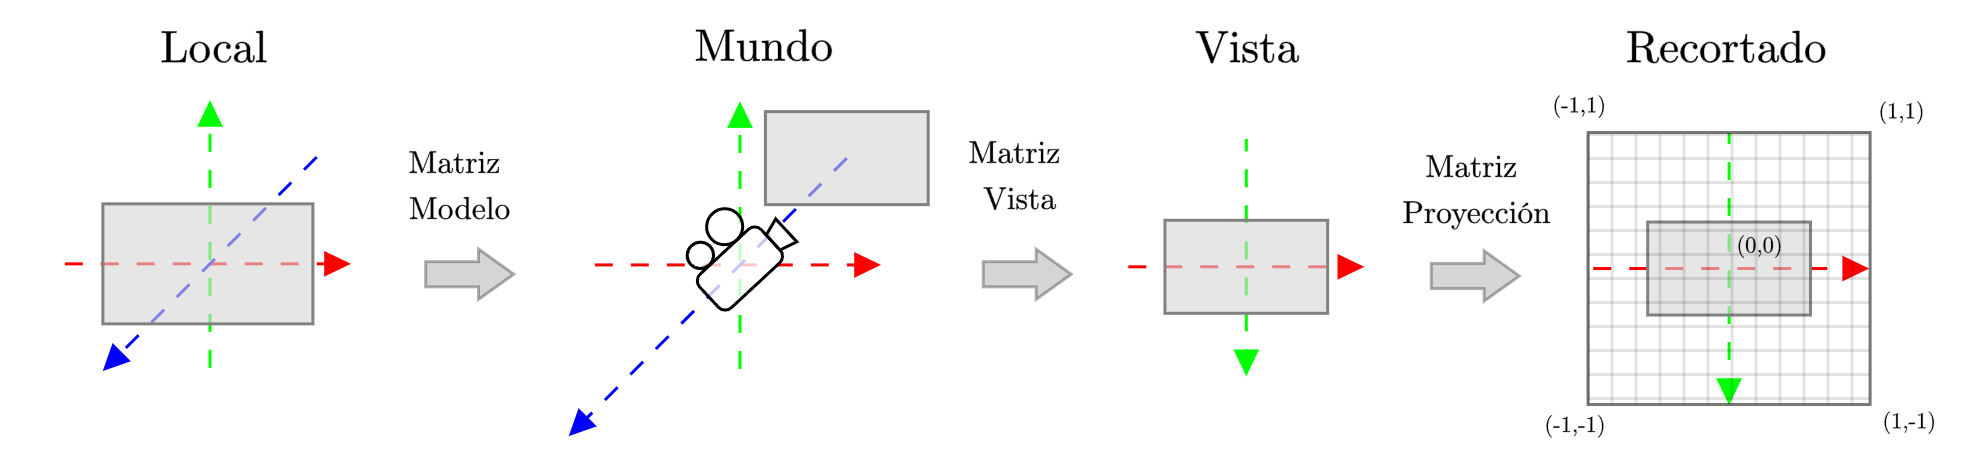
\includegraphics[width=\textwidth]{Plantilla-TFG-master/img/matrices2.png}
    \caption{Coordenadas locales a recortadas}
    \label{fig:matrices}
\end{figure}
\begin{itemize}
    \item \textbf{Matriz de modelo $\boldsymbol{M}$:} define la posición, orientación y escala del objeto en la escena. Se utiliza para pasar del coordenadas locales a coordenadas de mundo. En nuestro caso, si creamos el plano centrado en el origen, podemos simplemente tomar la matriz identidad de dimensión cuatro
    \begin{equation*}
        M = Id_{4\times 4}.
    \end{equation*}
    \item \textbf{Matriz de vista  $\boldsymbol{V}$:} define la posición y orientación de cada punto respecto a la cámara de la escena. Se utiliza para pasar de coordenadas de mundo a coordenadas de vista. Lo que ocurre en realidad es que la cámara está fija en el origen, y es el resto de la escena es la que se mueve respecto a ella. Por tanto, esta matriz contiene la posición y orientación inversa de la cámara. En nuestro caso, si queremos desplazar la cámara una unidad en el eje Z, la matriz de vista tendrá la forma
    \begin{equation*}
        V = \begin{pmatrix}
        1 & 0 & 0 & 0\\
        0 & 1 & 0 & 0\\
        0 & 0 & 1 & -1\\
        0 & 0 & 0 & 1
        \end{pmatrix}.
    \end{equation*}
    
    \item \textbf{Matriz de proyección:} define cómo la escena se proyecta en la pantalla, incluyendo el campo de visión, aspecto y planos cercano y lejano. Se utiliza para pasar de coordenadas de vista a coordenadas recortadas en función de las siguientes características del \textit{view-frustum}, la región del espacio de la escena que es visible por pantalla.
    \begin{itemize}
        \item Apertura vertical del campo de visión $\beta$ indicada como un ángulo entre $0$ y $180$ grados.
        \item Relación de aspecto $a$ entre el ancho $w$ y el alto $h$ del \textit{view-frustrum}.
        \item Límites cercano y lejano en el eje $Z$ cambiados de signo $n$ y $f$ del \textit{view-frustrum}.
    \end{itemize}
    La matriz se construye como
    \begin{equation*}
        M_P = \begin{pmatrix}
        \frac{c}{a} & 0 & 0 & 0\\
        0 & c & 0 & 0\\
        0 & 0 & \frac{n+f}{n-f} & \frac{2nf}{n-f}\\
        0 & 0 & -1 & 0
        \end{pmatrix}, \text{ donde } c = \coth\left({\frac{\beta}{2}}\right).
    \end{equation*}

    % \item \textbf{Matriz de ventana o \textit{viewport}:} se transforman las coordenadas de recortado a las coordenadas de dispositivo. Estas coordenadas están centradas en la esquina inferior izquierda de la pantalla y están en el rango $[0,r_x]\times [0,r_y]$, donde $r=(r_x,r_y)$ es la resolución de la pantalla.
\end{itemize}

\begin{figure}[ht!]
    \centering
    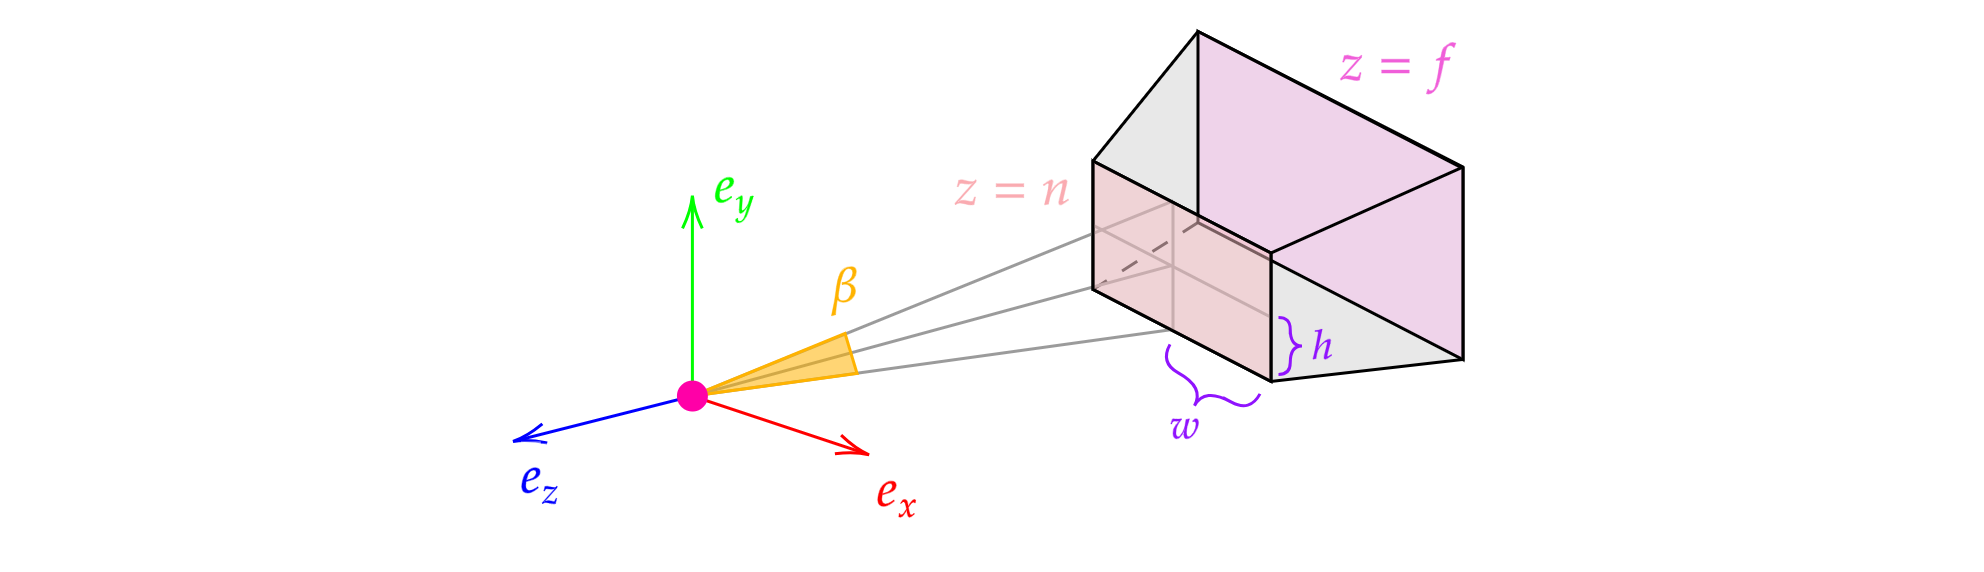
\includegraphics[width=\textwidth]{Plantilla-TFG-master/img/frustrum.png}
    \caption{Parámetros del \textit{view frustrum}}
\end{figure}

Con esta información ya podemos escribir nuestro \textit{vertex shader}, mostrado en la \autoref{fig:mainVS}.  
\begin{figure}[ht!]
    \centering
       \begin{algorithm}[H]
            \caption{Vertex Shader}
            \KwData{matriz de proyección $M_P$, matriz de vista $M_V$, matriz de modelo $M_M$, y coordenadas locales homogéneas del vértice $v_{loc}$}
            \KwResult{posición transformada del vértice actual en coordenadas homogéneas de mundo $v_{wc}$}
                $v_{wc} \gets M_P \cdot M_V \cdot M_M \cdot v_{loc}$
        \end{algorithm}
    \caption{Cuerpo del método \texttt{main} del \textit{vertex shader}}
    \label{fig:mainVS}
\end{figure}

Tras la ejecución del \textit{vertex shader} las coordenadas de recortado se transforman a coordenadas de dispositivo, que el \textbf{procesador de fragmentos o \textit{fragment shader}} recibirá como entrada. De él se ejecutará una instancia para cada píxel de la pantalla, y su objetivo es asignar a la variable $v_{loc}$ el color que el píxel tendrá como una terna RGBA, y será aquí donde hagamos todos los cálculos necesarios pare renderizar la superficie con \textit{spheretracing}. El primer paso para esto será definir un sistema de coordenadas dentro del propio lienzo con el que sea más cómodo trabajar que con el que ya disponemos a través de $v_{frag}$.\newline

Para obtener estas coordenadas, primero desplazamos el origen que nos proporciona $v_{frag}$ al centro de la pantalla usando el número de columnas y filas de pixels en la imagen, que deberemos pasar como parámetro al \textit{shader} y llamaremos \texttt{u\_resolution}, para posteriormente normalizar respecto a alguno de los ejes. Hacemos esto porque si intentamos normalizar sobre ambos ejes obtendremos coordenadas en el rango $[-0.5,0.5]^2$, y al no ser (en general) el lienzo cuadrado, la imagen se verá estirada en la dirección del eje más largo. Nosotros normalizaremos respecto al eje vertical, ya que en nuestro caso será siempre el menor. Esto nos dará como resultado unas coordenadas con valores en $\left[ -0.5\cdot aspect, 0.5\cdot aspect \right] \times [-0.5, 0.5]$, donde $aspect$ es el ratio de aspecto del lienzo, el resultado de dividir el ancho de la imagen por el alto, ambos medidos en pixels. Finalmente, para que la coordenada Y tome siempre valores en $[-1,1]$ multiplicamos por dos. Con esto conseguimos las coordenadas del centro del pixel en coordenadas normalizadas de dispositivo, similares a las de recortado pero divididas por la componente homogénea.
\begin{equation*}
    uv = \frac{2\cdot(v_{frag} - 0.5\cdot u\_resolution)}{u\_resolution_y}.
\end{equation*}

Hemos denotado a las coordenadas obtenidas como $uv$, haciendo referencia a la similitud que tienen con el uso que se le da a las coordenadas de textura habituales, ya que las vamos a usar para pintar sobre el lienzo como si de aplicar una textura se tratase. Cuando se trabaja con \textit{fragment shaders} la forma de debugear es dando colores a los pixels. En nuestro caso, podemos ver la diferencia entre ambos sistemas de coordenadas si usamos $uv$ como los canales rojo y verde del parámetro de salida $v_{col}$, superponiendo una rejilla construida usando la función módulo para apreciar si existe deformación, tal y como se muestra en la \autoref{fig:uv}. En ella podemos observar que si normalizamos sobre el eje horizontal, los verdes y amarillos no llegan a ser del todo intensos, ya que la componente del verde (la vertical) no llega a su valor máximo. Normalizando ambos ejes obtenemos el rango de colores completo, pero existe deformación en la rejilla debido a que el lienzo no es cuadrado. Finalmente, normalizando sobre el eje vertical obtenemos también el rango completo de colores, ya que los valores del eje horizontal que se salen del rango $[-1,1]$ son visualizados como si hubieran sido acotados en dicho intervalo, pero la rejilla se dibuja correctamente. En las siguientes secciones veremos cómo usar estas coordenadas para dibujar nuestra superficie sobre el lienzo.
\newline

\begin{figure}[htbp]
    \centering
    \begin{minipage}[b]{0.45\textwidth}
        \centering
        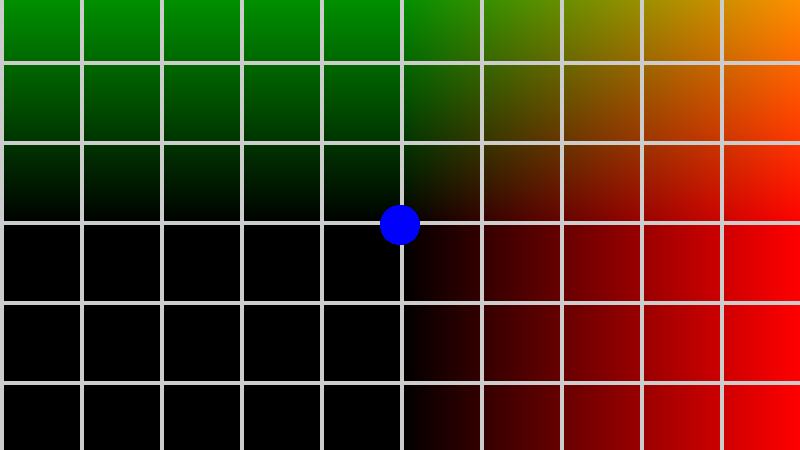
\includegraphics[width=\textwidth]{Plantilla-TFG-master/img/normX.png}
        \caption{Eje X}
    \end{minipage}
    \hfill
    \begin{minipage}[b]{0.45\textwidth}
        \centering
        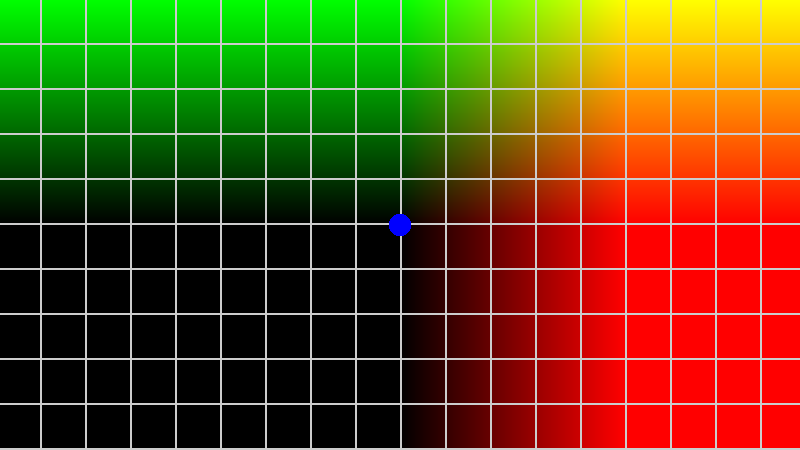
\includegraphics[width=\textwidth]{Plantilla-TFG-master/img/normY.png}
        \caption{Eje Y}
    \end{minipage}
    
    \medskip
    
    \begin{minipage}[b]{0.45\textwidth}
        \centering
        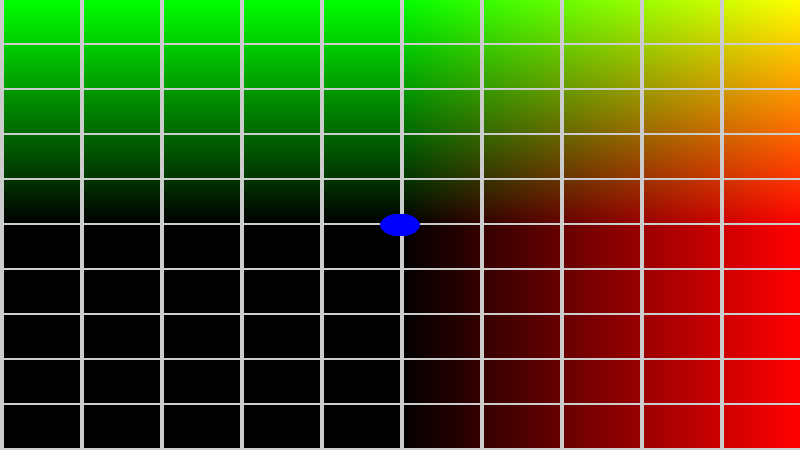
\includegraphics[width=\textwidth]{Plantilla-TFG-master/img/normXY.png}
        \caption{Ejes X e Y}
    \end{minipage}
    
    \caption{Normalización de coordenadas sobre distintos ejes}
    \label{fig:uv}
\end{figure}


\subsection{Generación de rayos primarios}
A partir de ahora, pensamos en nuestra escena no como en la que hemos definido el lienzo, sino aquella que queremos dibujar usando \textit{spheretracing} dada una función distancia con signo $\phi$. Esta escena estará definida en el espacio de coordenadas de mundo, el cual tiene un marco de referencia formado por tres vectores unitarios $B=\{e_x,e_y,e_z\}$ y un origen $o$, y colocaremos en ella los siguientes elementos (a partir de ahora supondremos que todas las tuplas de coordenadas son en coordenadas de mundo):
\begin{itemize}
    \item La \textbf{isosuperficie} $S_{\phi}$.
    \item \textbf{Plano de visión:} rejilla perpendicular al eje óptico de la cámara, donde cada uno de sus cuadrados corresponde a un píxel del lienzo.
    \item \textbf{Punto de la cámara $\boldsymbol{c_o}$:} punto del espacio desde donde se observa la escena.
    \item \textbf{Punto de atención o \textit{lookat point} $\boldsymbol{l}$:} hacia que punto del espacio debe mirar la cámara. En general tomaremos $l=o=(0,0,0)$.
\end{itemize}
La idea para conseguir representar la superficie consiste en trazar rayos a partir de $c_o$ hacia el centro de cada uno de los cuadrados del plano de visión, cada uno representando un píxel de la pantalla, de forma que si el rayo interseca con $S_\phi$ significa que ese píxel corresponde a un punto de la superficie, y será coloreado como tal.
\begin{figure}[h]
    \centering
    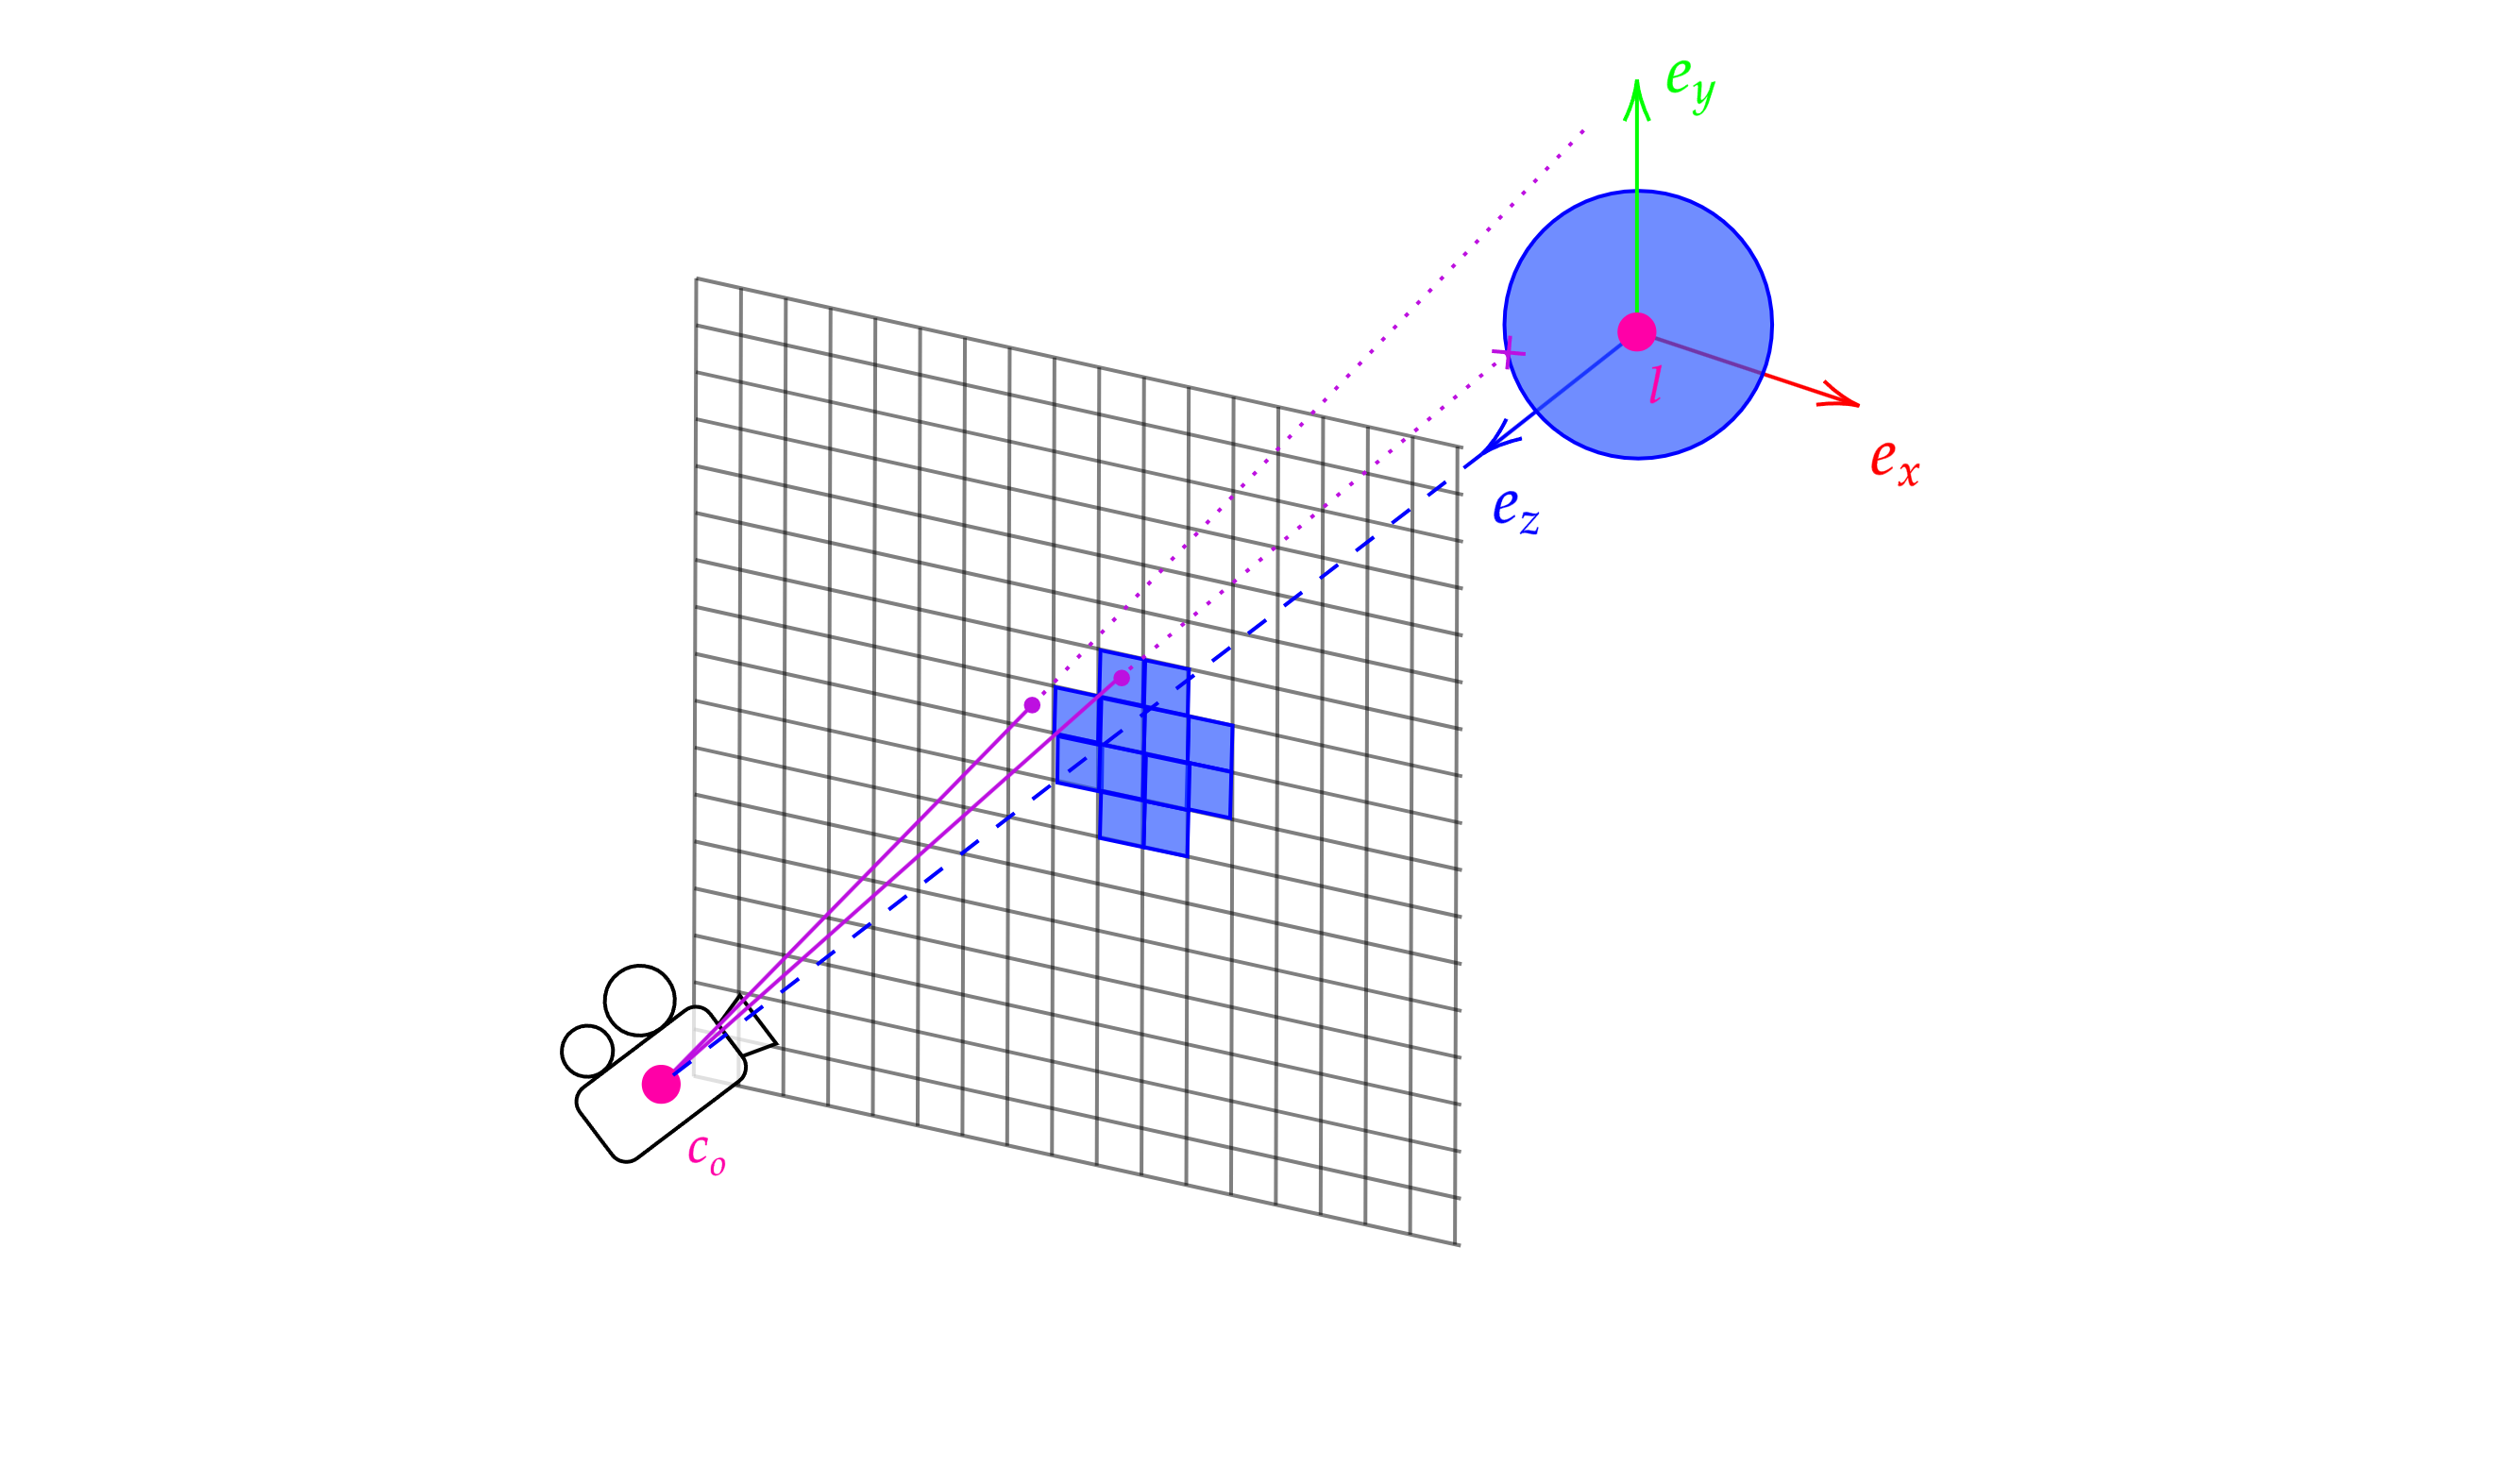
\includegraphics[width=\textwidth]{Plantilla-TFG-master/img/raymarch_fix.png}
    \caption{Trazado de rayos a través del plano de visión}
    \label{fig:raymarch1}
\end{figure}
\newline

Cada uno de estos rayos estará definido por un origen $r_o$ y una dirección $r_d$. El origen será siempre la posición de la cámara $c_o$, pero obtener la dirección requiere más trabajo. En el escenario descrito en la \autoref{fig:raymarch1}, donde $S_{\phi}$ es una esfera centrada en el origen y el observador se encuentra sobre el eje Z, dado que en todo momento conocemos las coordenadas de cada punto de la rejilla a través de $uv = (u,v)$, es claro que podemos tomar
$$r_d = (u,v,0) - c_0.$$ 
Una opción sería tomar $c_0 = (0,0,d)$, donde el valor $d$ es la distancia desde el punto del observador (foco de la proyección) al plano de visión. Modificar el valor de $d$ cambiaría los ángulos de apertura de visión horizontal y vertical, cambiando el tamaño aparente de los objetos proyectados. Es decir, $d$ actuaría como un control del campo de visión, de forma que cuanto mayor sea su valor mayores serán los ángulos de visión, y por tanto los objetos se verán más pequeños. Lo fijaremos a un valor de $1$. Sin embargo este escenario es el más sencillo posible, y si queremos poder mover la cámara manteniendo el punto de atención $l$ en el centro de la pantalla tendremos que poder trabajar con una orientación arbitraria suya. Para ello deberemos construir un marco de coordenadas de vista relativo a la cámara, que definiremos por una base ortonormal $\{f_1,f_2,f_3\}$ y el origen $c_0$.\newline

Para obtener el valor de los elementos de $f_1,f_2$ y $f_3$ empezamos obteniendo los siguientes vectores ortonormales.
\begin{itemize}
    \item \textbf{Vector director $\boldsymbol{c_d}$:} indica la dirección hacia la que mirará la cámara, que será paralela al eje $Z$ del marco de coordenadas de vista. Su valor vendrá dado por $c_d = l-c_o$.
    \item \textbf{\textit{Right vector} $\boldsymbol{c_r}$ }: paralelo al eje $X$ del marco de coordenadas de vista. Debe ser perpendicular tanto a $c_d$ como al vector \textit{view-up}. Este último, que denotaremos como $u$, es un vector libre que indica la dirección que el observador verá proyectada en vertical y apuntando hacia arriba en la imagen, y normalmente se toma el valor $u=(0,1,0)$ para que coincida con el eje $Y$. Al ser $c_r$ perpendicular al vector director y a \textit{view-up}, podemos obtenerlo como el producto vectorial de ambos: $c_r = u \times c_d$.
    \item \textbf{\textit{Up vector} $\boldsymbol{c_u}$}: paralelo al eje $Y$ del marco de coordenadas de vista. Como debe ser ortogonal a los otros dos, lo calculamos como $c_u = c_d\times c_r$.
\end{itemize}
A partir de estos vectores podemos obtener $\{f_1,f_2,f_3\}$ normalizándolos y teniendo en cuenta que el plano de visión y la cámara estarán orientados de forma opuesta:
\begin{equation*}
    f_1 = -\frac{c_r}{\Vert c_r\Vert} = -\frac{(0,1,0)\times c_d}{\Vert l-c_o\Vert},\quad 
    f_2 = \frac{c_u}{\Vert c_u\Vert } = f_3\times f_1, \quad
    f_3 = -\frac{c_d}{\Vert c_d\Vert} = -\frac{l-c_o}{\Vert l-c_o\Vert}. 
\end{equation*}
Ahora que tenemos el nuevo marco cartesiano, queda transformar el vector director original $r_d = (u,v,-1)$ a la base que acabamos de obtener. La matriz de cambio de base serán las coordenadas por columnas de $\{f_1,f_2,f_3\}$ escritas en función de $\{e_x,e_y,e_z\}$, que al ser la base del marco de coordenadas de mundo y al tratarse de una matriz de cambio de base entre dos marcos cartesianos, coincidirá con escribir por columnas $\{f_1,f_2,f_3\}$, de forma que
\begin{equation*}\label{eq:rayo}
    rayo = (u,v,-1)_{B}^t = \big(f_1\ \vert\  f_2\  \vert\  f_3\big) \cdot \begin{pmatrix}
        u\\
        v\\
        -1
    \end{pmatrix}.
\end{equation*}

\begin{figure}[ht!]
    \centering
    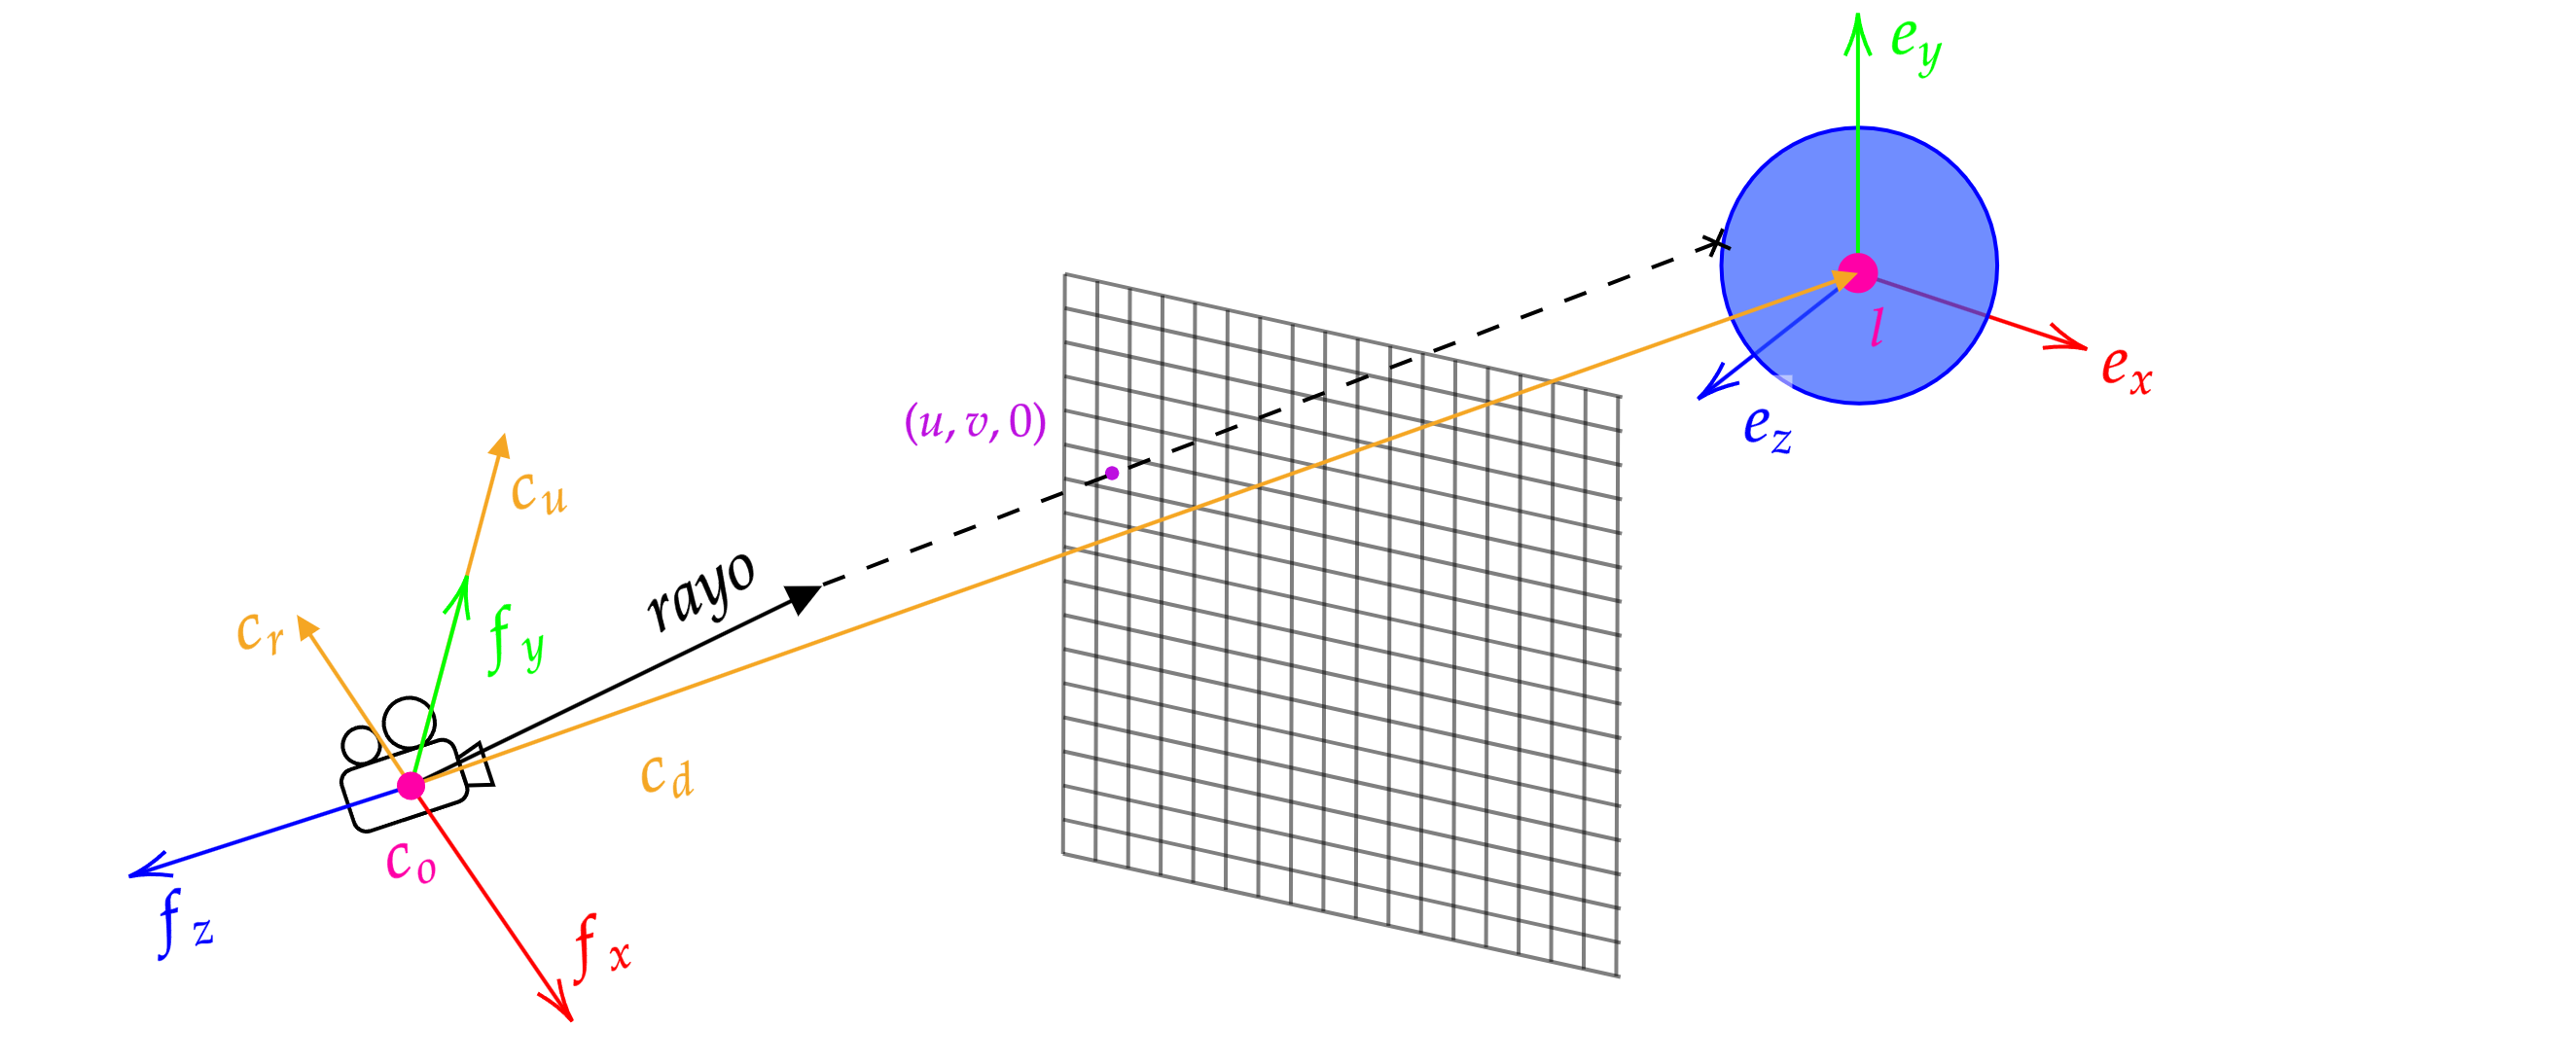
\includegraphics[width=\textwidth]{Plantilla-TFG-master/img/raydir_fix.png}
    \caption{Obtención de la dirección del rayo}
    \label{fig:raydir}
\end{figure}

\subsection{Algoritmos de intersección rayo-escena: \textit{raymarching} y \textit{spheretracing}}\label{sec:tracing}
Una vez que conocemos toda la información del rayo ya estamos en disposición de comprobar si este interseca con $S_{\phi}$. Para esto se pueden utilizar varios algoritmos, de entre los que estudiaremos el \textit{raymarching} y el \textit{spheretracing}. El método del \textit{spheretracing} es una variante del \textit{raymarching}, así que estudiaremos este primero.\newline

El \textbf{\textit{raymarching}} es un método iterativo: a partir de $c_o$, en cada iteración avanzamos en la dirección del rayo una distancia fija $\delta$. Evaluamos entonces nuestra SDF en la posición actual, de forma que si obtenemos un valor muy cercano a $0$ significará que hemos llegado a la isosuperficie. De lo contrario, repetimos el proceso hasta encontrar una intersección o superar un número máximo de iteraciones, en cuyo caso concluiremos que no hay intersección. La \autoref{a:raymarching} ilustra este procedimiento, donde \texttt{DibujarSuperficie()} y \texttt{DibujarFondo()} devuelven ternas RGBA que serán asignadas al píxel actual dependiendo de si hay intersección o no.\newline

\begin{figure}[ht!]
    \centering
    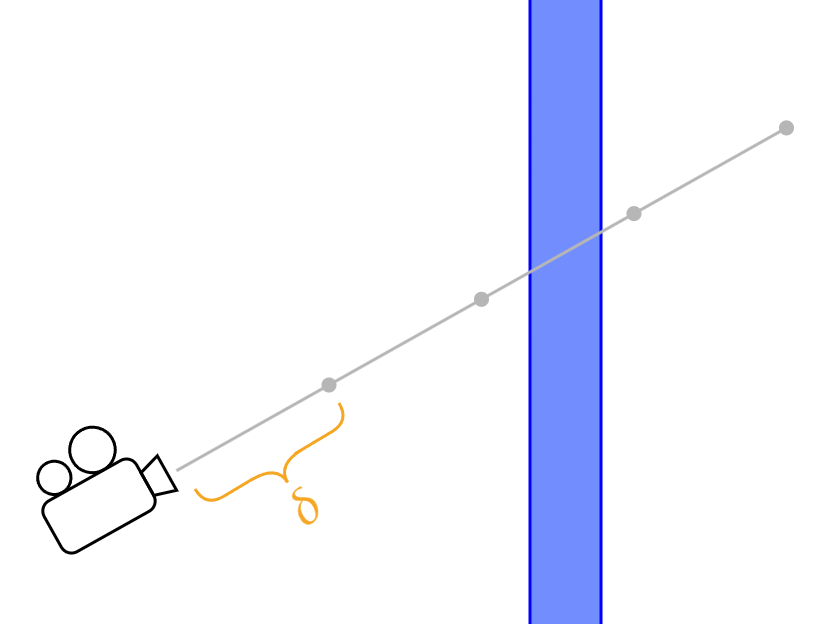
\includegraphics[width=0.4\textwidth]{Plantilla-TFG-master/img/miss.png}
    \caption{Pérdida de intersección en \textit{raymarching} para valores elevados de $\delta$}
    \label{fig:missInter}
\end{figure}

\SetKwComment{Comment}{// }{}
\begin{figure}[ht!]
    \centering
    \begin{minipage}{0.58\textwidth}
        \begin{algorithm}[H]
            \caption{Raymarching}
                \KwData{origen del rayo $c_o$, dirección del rayo $v$}
                \KwResult{terna RGB con el color del píxel actual}
                
                $d \gets 0$ \Comment{distancia total}
                
                \For{i $\in$ MAX\_ITERACIONES} {
                    $p \gets c_o +d\cdot v$
                    
                    sdf $\gets \phi(\text{p})$
                    
                    \If{sdf $< \varepsilon$}{
                       \Return{DibujarSuperficie($p,v,sdf$)}
                    }
            
                    $d\gets d + \delta$\;
            
                    \If{$d >$ MAX\_DISTANCIA}{
                        \Return{DibujarFondo()}
                    }
                }
        \end{algorithm}
    \end{minipage}%
    \hfill
    \begin{minipage}{0.4\textwidth}
        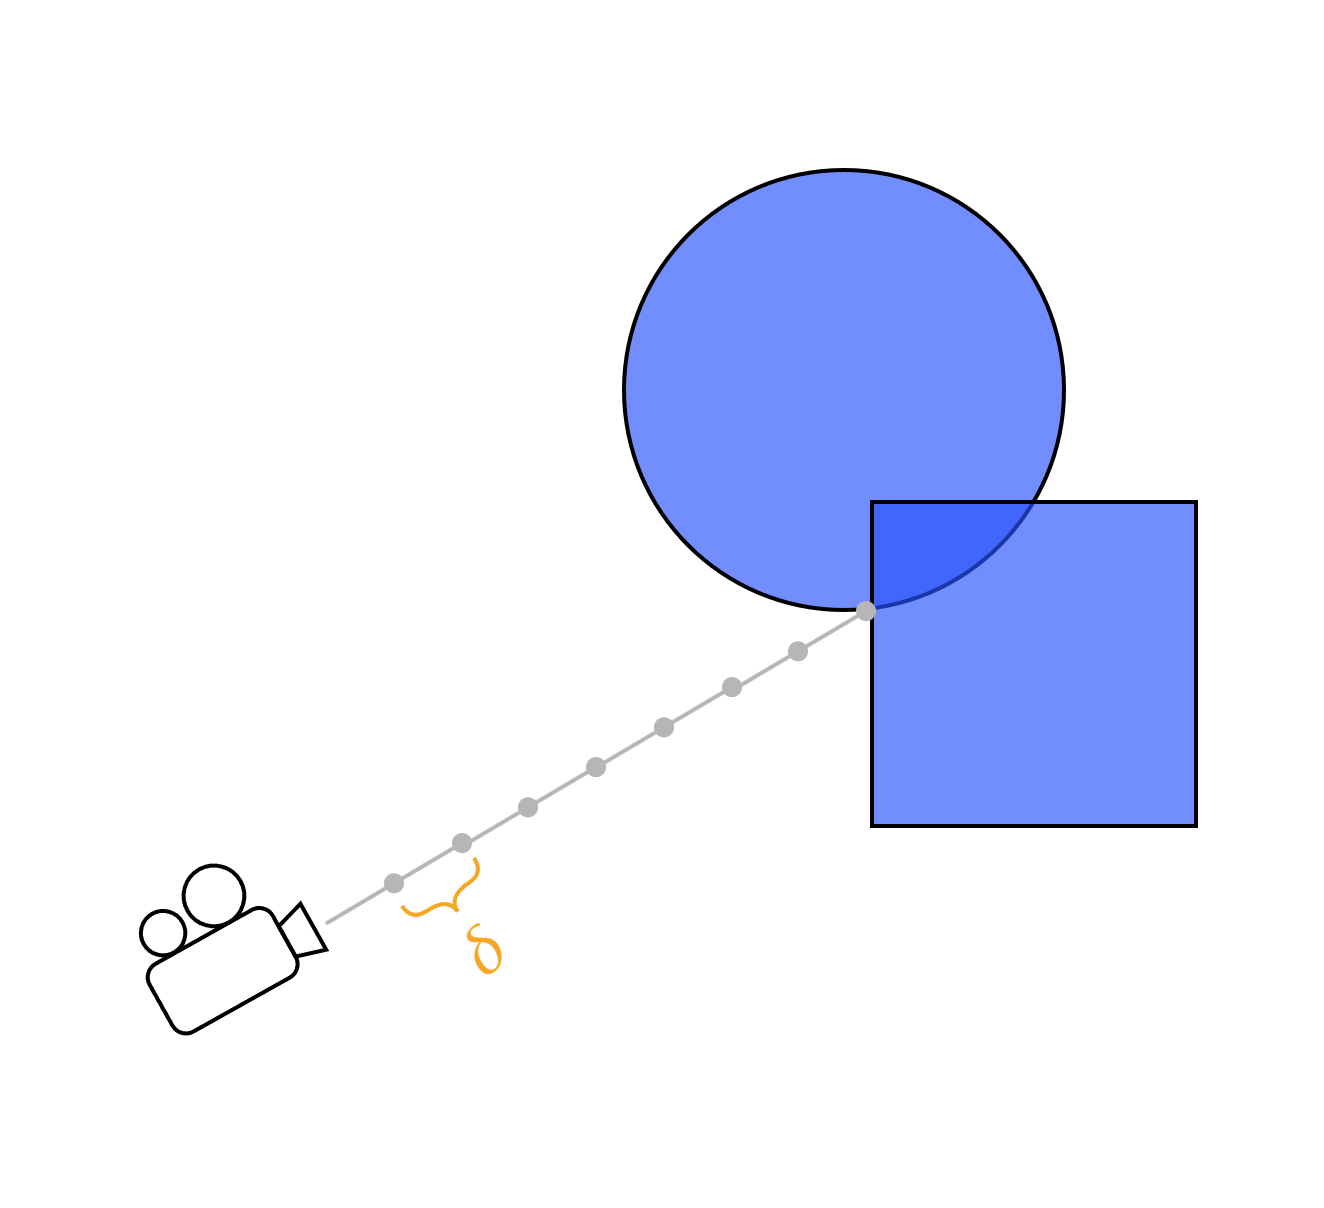
\includegraphics[width=\textwidth]{raymarching.png}
    \end{minipage}
    \caption{Algoritmo de \textit{raymarching}}
    \label{a:raymarching}
\end{figure}

Una desventaja de esta técnica es que puede ser bastante lenta, ya que cuanto más alejados estén los puntos de $S_\phi$ del observador, mayor es el número de iteraciones necesarias para encontrar la intersección en caso de que la haya. En el peor de los casos en el que tal intersección no exista, se habrá realizado el número máximo de iteraciones, que además será bastante alto debido a que el valor de incremento $\delta$ debe ser pequeño si no queremos perder ninguna intersección, como ocurre en la \autoref{fig:missInter}.\newline

Como solución a este problema aparece el \textit{spheretracing}, que reduce drásticamente el número de iteraciones, y por tanto de evaluaciones de $\phi$, necesarias para detectar la intersección. Su funcionamiento es similar al \textit{raymarching}, con la diferencia de que el incremento en la posición del rayo no es fija, sino que es la máxima que podemos tomar en cada momento asegurándonos de no perdernos una intersección. Esta distancia será la mínima del punto actual del rayo a $S_\phi$, que no es más que evaluar $\phi$ en dicho punto.\newline

Este será por tanto el algoritmo que utilizaremos para detectar qué pixels de la pantalla corresponden a la superficie $S_{\phi}$, y se encuentra descrito con detalle en la \autoref{a:spheretracing}. 
Con esto al fin podemos describir la forma que tendrá nuestro \textit{fragment shader} en la \autoref{fig:mainFS}. Claro está que esta versión todavía no es funcional, pues no sabemos qué forma tiene \texttt{DibujarSuperficie}, y como mucho podremos obtener una imagen que separe la isosuperficie del fondo usando colores planos como muestra la \autoref{fig:planos} para una esfera centrada en el origen. Veremos como mejorar esto en la próxima sección.

\begin{figure}[ht!]
    \centering
    \begin{minipage}{0.58\textwidth}
       \begin{algorithm}[H]
            \caption{Spheretracing}
                \KwData{origen del rayo $c_o$, dirección del rayo $v$}
                \KwResult{terna RGB con el color del píxel actual}
                $d \gets 0$ \Comment{distancia actual}
                
                \For{i $\in$ MAX\_ITERACIONES} {
                    $p \gets c_o + d \cdot v$
                    
                    $sdf \gets \phi(p)$
                    
                    \If{sdf $< \varepsilon$}{
                       \Return{$DibujarSuperficie(p,v,sdf)$}
                    }
            
                    $d \gets$ d + sdf
            
                    \If{$d >$ MAX\_DISTANCIA}{
                        \Return{$DibujarFondo()$}
                    }
                }
        \end{algorithm}
    \end{minipage}%
    \hfill
    \begin{minipage}{0.4\textwidth}
        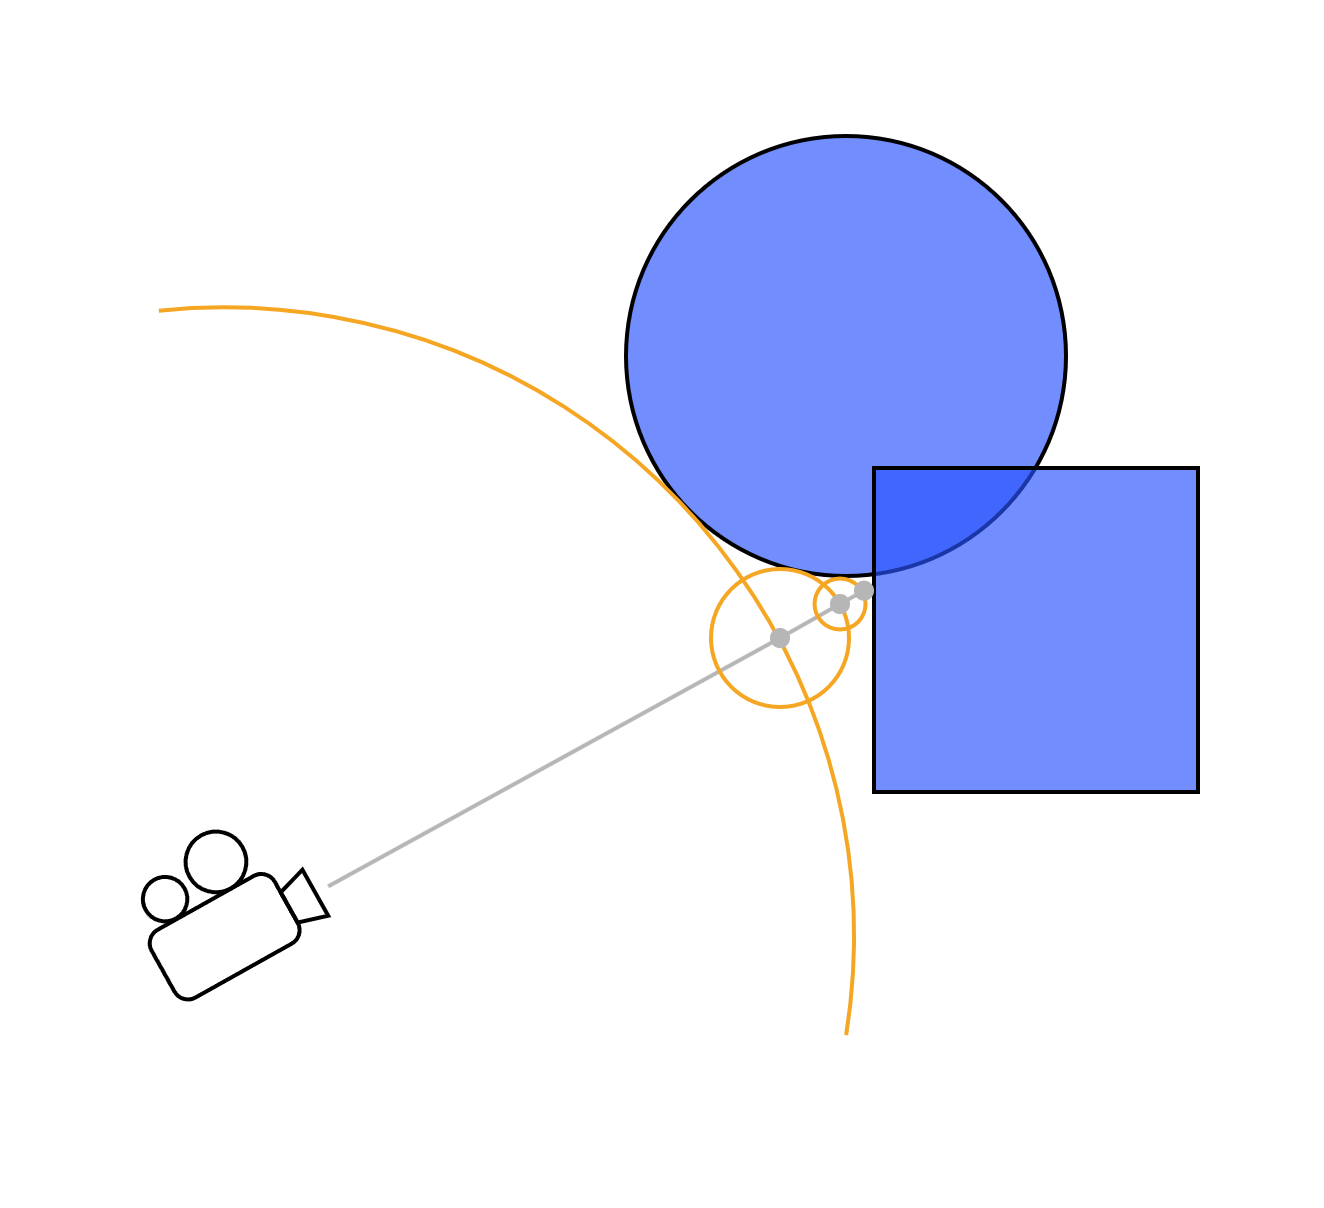
\includegraphics[width=\textwidth]{spheremarching.png}
    \end{minipage}
    \caption{Algoritmo de \textit{spheretracing}}
    \label{a:spheretracing}
\end{figure}

\begin{figure}[ht!]
    \centering
    
       \begin{algorithm}[H]
            \caption{Fragment Shader}
            \KwData{coordenadas de dispositivo $v_{frag}$ del píxel actual}
            \KwResult{color del píxel actual como terna RGBA $v_{col}$}

                $c_0 \gets $ posición de cámara en función de la entrada del ratón

                $l\gets $ punto de atención elegido por el usuario
                
                $uv \gets 2\cdot \frac{v_{frag} - 0.5\cdot u\_resolution}{u\_resolution_y}$\\[5pt]

                $f_1,\ f_2,\ f_3 \gets CalcularMarcoCartesiano(c_0, l)$
                
                $r_d \gets (f_1\ \vert \ f_2\ \vert \ f_3)\cdot normalizar ((uv_x, uv_y,-1))$\\[5pt]

                $color \gets$ spheretracing$(c_0, r_d)$\\[5pt]

                $v_{col} \gets (color_x, color_y, color_z, 1)$
        \end{algorithm}
    \caption{Cuerpo del método \texttt{main} del \textit{fragment shader}}
    \label{fig:mainFS}
\end{figure}


\begin{figure}[ht!]
    \centering
    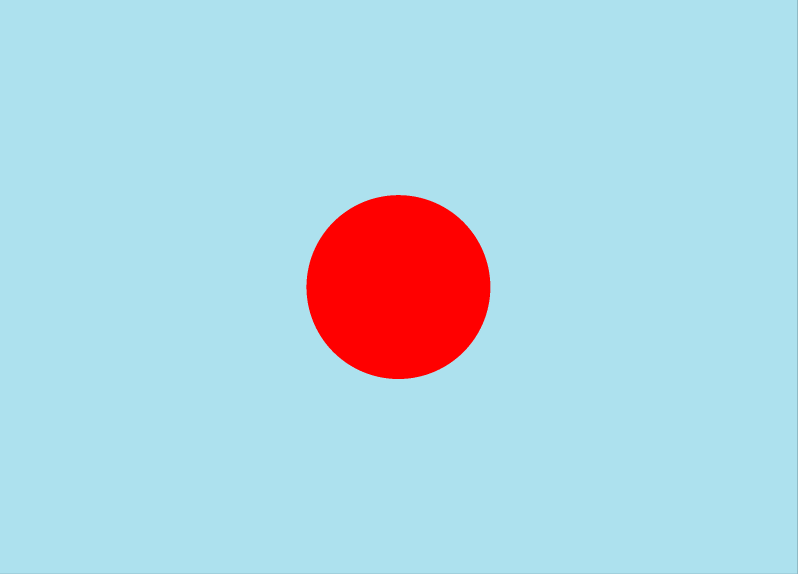
\includegraphics[width=0.8\textwidth]{Plantilla-TFG-master/img/escenaPlana.png}
    \caption{Resultado de \textit{spheretracing} asignando colores planos}
    \label{fig:planos}
\end{figure}


\section{Modelos de iluminación y sombras}\label{sec:ilum}
Ya sabemos qué pixels pertenecen a la superficie, pero no de qué color deben dibujarse. En esta sección estudiaremos diversas técnicas que en conjunto nos permitirán simular de forma plausible qué ocurre cuando se añaden a la escena una o varias fuentes de luz.


\subsection{Modelos de Blinn y Blinn-Phong}
Empezamos viendo cómo las fuentes de luz presentes en la escena iluminan directamente la superficie. Hay multitud de modelos que simulan este comportamiento de forma más o menos realista, siendo uno de los más extendidos el renderizado basado en física (\textit{physically based rendering} o PBR). Sin embargo, este y otros acercamientos similares son utilizados cuando se requiere de un alto grado de fidelidad y adaptabilidad. Nosotros usaremos el modelo de reflexión de Blinn-Phong \cite{apuntes:ig}, también popular pero mucho más simple y computacionalmente menos costoso. A su vez este modelo se basa en el de Blinn, el cual pasamos a estudiar a continuación. \newline

Vamos a considerar que nuestra escena consta de los siguientes elementos.
\begin{itemize}
    \item La \textbf{isosuperficie} $S_{\phi}$ como único objeto a ser dibujado (aunque el modelo es válido para cualquier número de objetos en escena).
    \item Un \textbf{observador} que se encuentra en la posición $c_o\in\R^3$ mirando a un punto $p\in \R^3$.
    \item Un número finito $n$ de \textbf{fuentes de luz}. Llamaremos $l_i$ con $i\in \{1,\dots, n\}$ a los vectores normalizados que apuntan desde $p$ a la posición de cada fuente.
\end{itemize}

Empecemos comprendiendo el fenómeno físico que tratamos de simular. La luz que generan las fuentes no es más que radiación electromagnética. De forma ideal, esta radiación se puede ver como un flujo en el espacio de partículas llamadas \textbf{fotones} que siguen trayectorias rectilíneas a la par que interaccionan con el entorno. Cada una de estas partículas tendrá una energía radiante única en función de su longitud de onda, que irá transfiriendo a aquellos objetos con los que interaccione.

\begin{definicion}[Radiancia]
    Dado un punto $p\in\R^3$, llamamos \textbf{radiancia} a la densidad de energía radiante por unidad de tiempo de los fotones que pasan por un entorno de $p$ en una determinada dirección $v\in\R^3$ con $\Vert v\Vert = 1$. La denotaremos $L(p,v)$, y será representada mediante una terna RGB no acotada. Podemos distinguir a su vez varios tipos de radiancia.
    \begin{itemize}
        \item \textbf{Radiancia emitida $\boldsymbol{L_E(p,v)}$:} radiancia que emite el propio objeto, también llamada emisividad. Normalmente es de intensidad baja y la consideraremos constante.
        \item \textbf{Radiancia incidente $\boldsymbol{L_{I}}(p,v)$:} radiancia que recibe el punto $p$ desde la dirección $v$. 
        \item \textbf{Radiancia reflejada $\boldsymbol{L_{R}}(p,v)$:} cantidad de la radiancia incidente en $p$ que se refleja en la dirección $v$. 
\end{itemize}
\end{definicion}

El objetivo del modelo será por tanto describir la radiancia que percibe el observador desde su posición en el punto $p$. Para ello, se llevan a cabo una serie de simplificaciones:
\begin{itemize}
    \item En un modelo físicamente correcto la luz reflejada en cada punto se dispersaría por el entorno, contribuyendo a la radiancia incidente en otros puntos de la escena. Sin embargo, nosotros no consideraremos la radiancia incidente que no provenga directamente de fuentes de luz. Incluso teniendo un solo objeto en escena como es nuestro caso este modelo es mejorable, pues el objeto puede reflejar radiancia sobre sí mismo. Por tanto, usaremos una radiancia ambiente constante $L_A$ para suplir esta iluminación indirecta.
    \item La radiancia se conserva en el espacio entre objetos.
    \item Las fuentes de luz son direccionales, de forma que no serán visibles en la escena. Además supondremos que emiten una radiancia constante $S_i$ para $i\in \{1,\dots, n\}$.
    \item No se consideran objetos con transparencia.
\end{itemize}
Es natural pensar que la radiancia percibida en un punto $p\in \R^3$ será la suma de la radiancia que emita y la que sea capaz de reflejar. Así, teniendo en cuenta las consideraciones anteriores tenemos que
\begin{equation*}
    L(p,v) = L_A + L_E + \sum_{i=1}^n L_R(p,l_i).
\end{equation*}
Como $L_A$ y $L_E$ son constantes solo nos falta estudiar cómo obtener la \textbf{radiancia reflejada} para cada fuente de luz. Para ello fijamos un índice $m\in \{1,\dots,n\}$ y suponemos a partir de ahora que $p\in S_{\phi}$, pues de lo contrario

\begin{equation*}
    L(p,v) = L_A,\ p\in \R^3\setminus S_{\phi},
\end{equation*}
ya que la única luz que se puede reflejar es la del ambiente y ya está siendo considerada con $L_A$, y al trabajar únicamente con fuentes de luz direccionales $L_E=0$. \newline

Sabemos que cada objeto refleja la luz de manera distinta en función de su material y las propiedades de la fuente. Para representar este comportamiento definimos una función que indique la fracción de radiancia proveniente de $l_m$ que se refleja en un punto $p$ en la dirección $v$ para cada fuente de luz
\begin{equation*}
    f_r \colon \R^3\times \R^3\times \R^3 \to \R^3.
\end{equation*}
Así, la radiancia reflejada es
\begin{equation*}
    L_R(p,v,l_m) = S_m\cdot f_r(p,v,l_m).
\end{equation*}

Podemos distinguir diferentes tipos de reflexión, cada uno contribuyendo de forma diferente a la radiancia reflejada final.

% donde $f_a$, $f_d$ y $f_e$ representan la fracción de radiancia reflejada para cada uno de los tipos de reflexión que podemos distinguir y listamos a continuación. 
\begin{itemize}
    \item \textbf{Reflexión ambiental:} cantidad de iluminación indirecta proveniente de la fuente de luz que refleja el objeto. Al igual que hicimos con $L_A$, tomaremos un valor constante $R_A$ para ella, de forma que la fracción de radiancia ambiental reflejada será
    \begin{equation*}
        f_{ra} =  R_A \in \R^3.
    \end{equation*}
    \item \textbf{Reflexión especular:} define cómo se refleja la luz en objetos brillantes teniendo en cuenta la posición de la fuente de luz y la del observador. Según la ley de refracción, el ángulo de incidencia de la luz será igual al de reflexión, luego podemos obtener la dirección de reflexión $r_m$ reflejando $l_m$ sobre el vector normal unitario en $p$ de la superficie, que llamaremos $N_p$. Así,
    
    \begin{equation*}
        r_m = 2(l_m\cdot N_p)N_p - l_m \in \R^3.
    \end{equation*}

    Sin embargo, solo queremos que haya reflejos en los puntos orientados hacia la fuente de luz y cuando $r_m$ haya sido reflejado en una dirección que el observador pueda apreciar, siendo la intensidad del reflejo mayor cuanto más alineado esté el observador con el vector reflejado. Esto equivale a que se cumpla
    \begin{equation*}
        N_p\cdot l_m >0 \quad \text{ y }\quad  R_m \cdot v>0.
    \end{equation*}
    Para controlar el color y la intensidad de los reflejos usaremos una radiancia $R_E$, de forma que podemos expresar la fracción de radiancia especular reflejada como
    \begin{align*}
        f_{re} \colon \R^3\times \R^3\times \R^3 &\to \R^3,\\
        (p,v,l_m) &\mapsto R_E \cdot \Max(0,l_m\cdot N_p) \cdot \Max(0,r_m \cdot v).
    \end{align*}
    \item \textbf{Reflexión difusa:} modela cómo se refleja la luz en objetos mates en función de la posición de la fuente de luz. Al contrario de lo que ocurre con la reflexión especular, debido a la irregularidad de la superficie del objeto la luz no se refleja en una sola dirección, haciendo que se disperse en direcciones impredecibles. Este comportamiento se simula a través de una radiancia $R_D$ que represente el valor promedio resultado de estos reflejos, y que consideraremos constante. Al igual que antes, solo queremos que el punto esté iluminado cuando esté de cara a la fuente de luz, obteniendo la mayor cantidad de luz cuando está alineado con la fuente. Así, la fracción de radiancia difusa será
    \begin{align*}
        f_{rd} \colon \R^3\times \R^3\times \R^3 &\to \R^3,\\
        (p,v,l_m) &\mapsto R_D\cdot \Max(0,l_m \cdot N_p).
    \end{align*}
\end{itemize}

\begin{figure}[ht!]
    \centering
    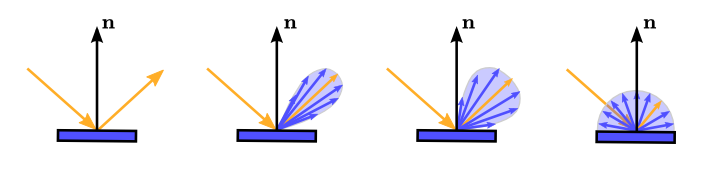
\includegraphics[width=0.85\textwidth]{Plantilla-TFG-master/img/glossyTodiffuse.png}
    \caption{Reflexión de un rayo en una superficie progresivamente más mate \cite{especular}}
    \label{fig:miss}
\end{figure}

\begin{observacion}
    Es necesario que los vectores $l_i$, $v$ y $N_p$ sean unitarios, pues de lo contrario su producto escalar no coincidiría con el coseno del ángulo que forman.
\end{observacion}

En vista de las definiciones anteriores, podríamos simplemente definir
\begin{equation*}
    f_r(p,v,l_m) = f_{ra}+f_{re}(p,v,l_m) + f_{r_d}(p,v,l_m).
\end{equation*}

De esta forma, para diferenciar entre un material totalmente mate como el yeso y uno especular como el metal bastaría tomar valores de $R_D$ y $R_E$ tal que $\Vert R_D\Vert \gg \Vert R_E\Vert$. Sin embargo, a la hora de comparar materiales especulares podríamos observar que aunque ambos generen zonas brillantes no lo hagan de la misma forma. Por ejemplo, tanto el mármol como el metal generan brillos sobre su superficie, pero en el caso del metal estos son más pequeños y brillantes debido a que se trata de un material más pulido. Por tanto, para añadir control sobre el tamaño e intensidad de estas zonas brillantes introducimos el \textbf{coeficiente de brillo} $\alpha \in \R$ en la expresión de $f_{re}$, de forma que cuanto mayor sea su valor más pequeños e intensos serán los brillos generados. En la \autoref{fig:parametrosEspecular} podemos ver el efecto que tienen $R_E,R_D$ sobre la radiancia reflejada \cite{especular}.\newline

\begin{definicion}
    Dado un objeto, definimos su \textbf{material} como la tupla $\{R_A,R_E,R_D,\alpha \}$.
\end{definicion}

Una vez asociado un material a $S_{\phi}$ podemos escribir la expresión final para $f_r$:

\begin{align}\label{eq:fr}
    f_r(p,v,l_i) &= f_{ra} &+\ & f_{re}(p,v,l_i) &+\ &f_{r_d}(p,v,l_i)\\
                 &= R_A    &+\ & R_E \cdot \Max(0,l_i\cdot N_p) \cdot \Max(0,r_i \cdot v)^{\alpha} &+\  &R_D\cdot \Max(0,l_i\cdot N_p). 
\end{align}

\begin{figure}[!h]
     \begin{minipage}[c]{0.45\linewidth}
        \centering
        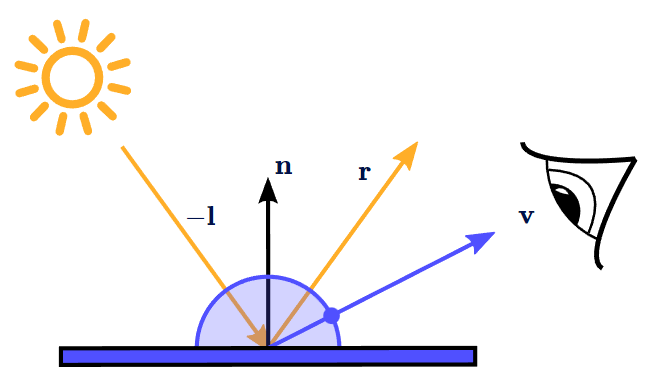
\includegraphics[width=0.95\textwidth]{Plantilla-TFG-master/img/ks0kd1.png}
        \caption{$\Vert R_E\Vert = 0$}
     \end{minipage}
     \begin{minipage}[c]{0.45\linewidth}
        \centering
        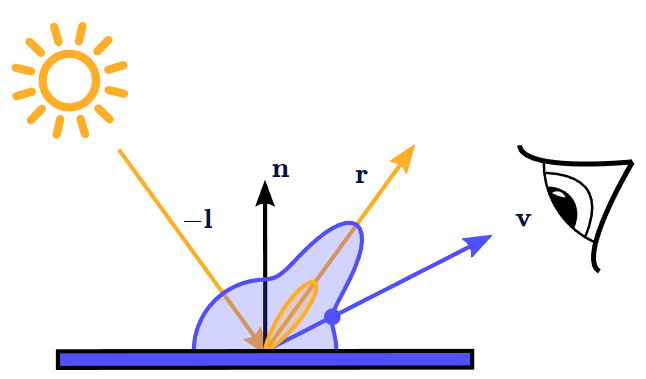
\includegraphics[width=0.95\textwidth]{Plantilla-TFG-master/img/ks1kd1.png}
        \caption{$\Vert R_E\Vert =\Vert R_D\Vert$ y $\alpha$ grande}
     \end{minipage}
     \begin{minipage}[c]{0.45\linewidth}
        \centering
        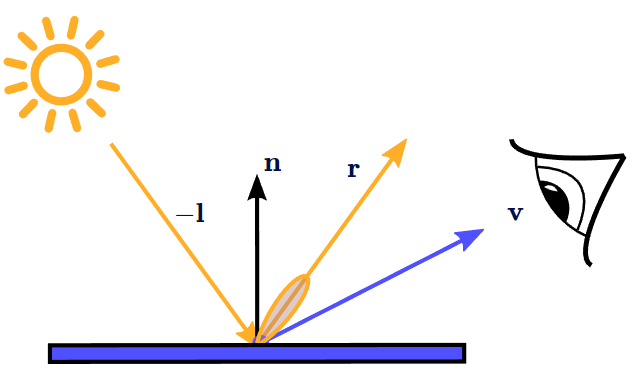
\includegraphics[width=0.95\textwidth]{Plantilla-TFG-master/img/ks1kd0.png}
        \caption{$\Vert R_D\Vert = 0$}
     \end{minipage}
     \begin{minipage}[c]{0.45\linewidth}
        \centering
        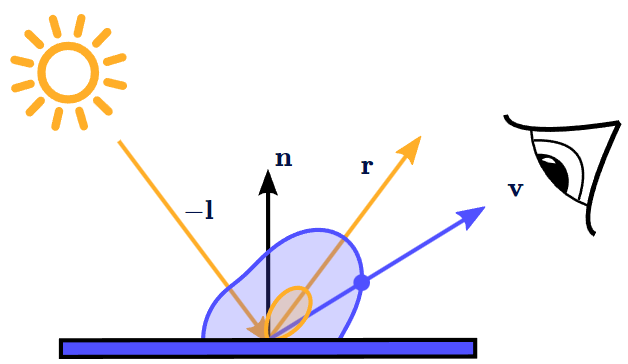
\includegraphics[width=0.95\textwidth]{Plantilla-TFG-master/img/ks1kd1a0.png}
        \caption{$\Vert R_E\Vert =\Vert R_D\Vert$ y $\alpha$ pequeño}
     \end{minipage}
     % \begin{minipage}[c]{0.45\linewidth}
     %    \centering
     %    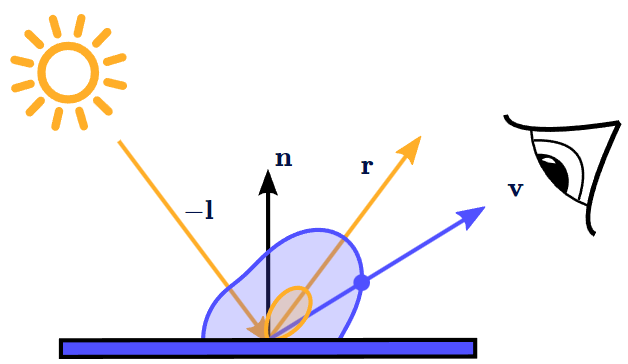
\includegraphics[width=0.95\textwidth]{Plantilla-TFG-master/img/ks1kd1a0.png}
     %    \caption{$k_s = 1$ y $k_d = 0$}
     % \end{minipage}
     \caption{Ejemplo de distintos valores para $R_E,R_D$ y $\alpha$}
     \label{fig:parametrosEspecular}
\end{figure}

Recogemos los resultados obtenidos en la siguiente definición.
\begin{definicion}[Modelo de Blinn]\label{def:blinn} La radiancia percibida en el punto $p\in\R^3$ desde la dirección $v\in\R^3$ con $\Vert v\Vert = 1$ según el modelo de Blinn viene dada por
    \begin{equation*}
        L(p,v) = L_A+L_E+ \sum_{i=0}^n S_i \Bigg[ k_aR_A + \Max(0,l_i\cdot N_p) \Big( k_dR_D + k_eR_E\cdot \Max(0,r_i\cdot v) \Big) \Bigg],
    \end{equation*}

    donde:
    \begin{itemize}
        \item $n \in \N$ es el número de fuentes de luz y $l_i \in R^3$ es el vector normalizado que apunta a $p$ desde cada una de ellas,
        \item $L_A,L_E \in \R^3$ son ternas RGB no acotadas representando la radiancia ambiente y emitida respectivamente,
        \item $S_i \in \R^3$ es una terna RGB no acotada representando la radiancia emitida por la fuente de luz $i$-ésima,
        \item $\alpha \in \R$ es el coeficiente de brillo,
        \item $R_A,R_D,R_E \in \R^3$ son ternas RGB (no acotadas) representando la radiancia reflejada de forma ambiental, difusa y especular respectivamente,
        \item $N_p$ es el vector normal de la superficie en $p$ y $r_i$ es el vector $l_i$ reflejado sobre $N_p$.
    \end{itemize}
\end{definicion}

En 1975 Phong \cite{phong} introdujo una variante a este modelo que hoy conocemos como \textbf{modelo de Blinn-Phong}. Su única diferencia con el de Blinn consiste en el uso del llamado \textit{halfway vector}
\begin{equation*}
    h_m = \frac{l_m + v}{\Vert l_m + v\Vert}.
\end{equation*}

Ahora, en lugar de usar el valor $r_m\cdot v$ hacemos que el brillo sea proporcional al coseno del ángulo entre $h_m$ y $N_p$, de forma que no depende del punto $p$ y solo necesita ser calculado una vez. En la \autoref{fig:phong} podemos ver el comportamiento de $h_m$ para distintas configuraciones de $l_m$ y $v$.
\begin{figure}[!h]
     \begin{minipage}[c]{0.32\linewidth}
        \centering
        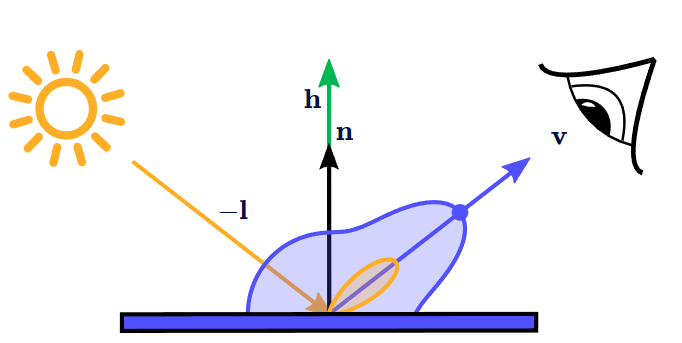
\includegraphics[width=0.95\textwidth, align=b]{Plantilla-TFG-master/img/phong1.png}
     \end{minipage}
     \begin{minipage}[c]{0.32\linewidth}
        \centering
        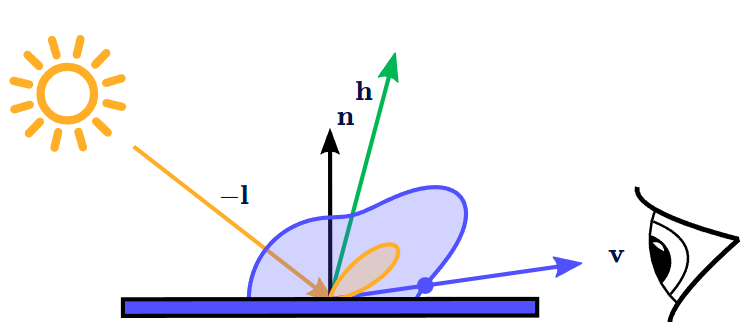
\includegraphics[width=0.95\textwidth, align=b]{Plantilla-TFG-master/img/phong2.png}
     \end{minipage}
     \begin{minipage}[c]{0.32\linewidth}
        \centering
        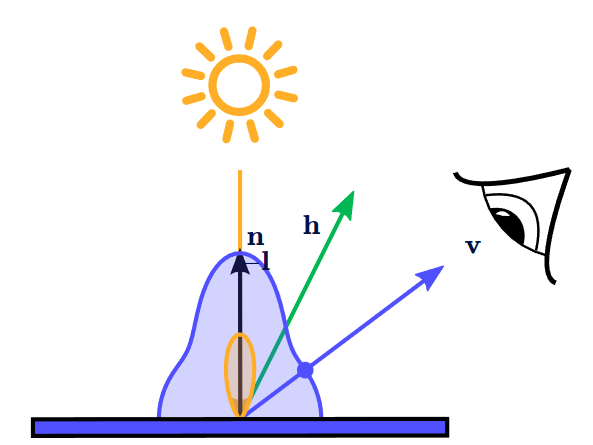
\includegraphics[width=0.95\textwidth, align=b]{Plantilla-TFG-master/img/phong3.png}
     \end{minipage}
     \caption{Comportamiento de  $h_m$ con $\Vert R_S\Vert =\Vert R_D\Vert$}
     \label{fig:phong}
\end{figure}

Aunque pueda parecer una simplificación del modelo de Blinn, lo cierto es que produce resultados más convincentes que este. En particular, mientras que el modelo de Blinn siempre produce brillos redondos en superficies planas, el de Blinn-Phong los genera con una forma más elíptica cuando se observa la superficie desde un ángulo acusado, como se observa en la \autoref{fig:difBlinn}. 

\begin{figure}[!h]
     \begin{minipage}[c]{0.49\linewidth}
        \centering
        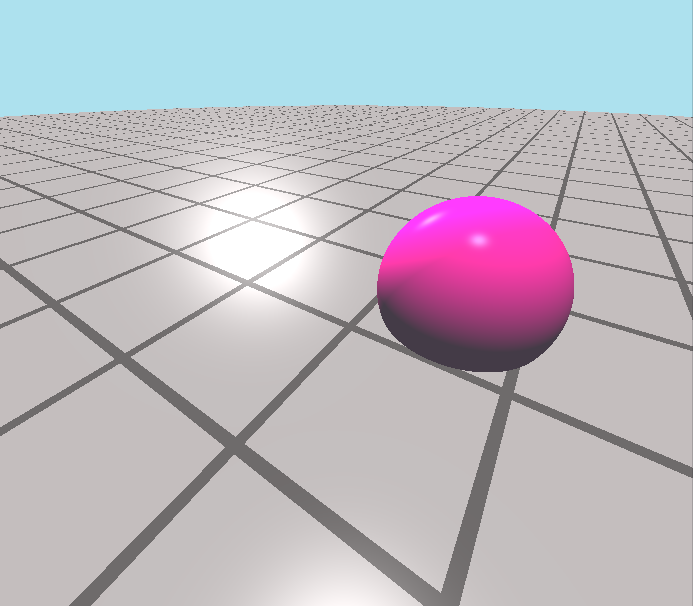
\includegraphics[width=0.9\textwidth]{Plantilla-TFG-master/img/compB.png}
        \caption{Blinn}
     \end{minipage}
     \begin{minipage}[c]{0.49\linewidth}
        \centering
        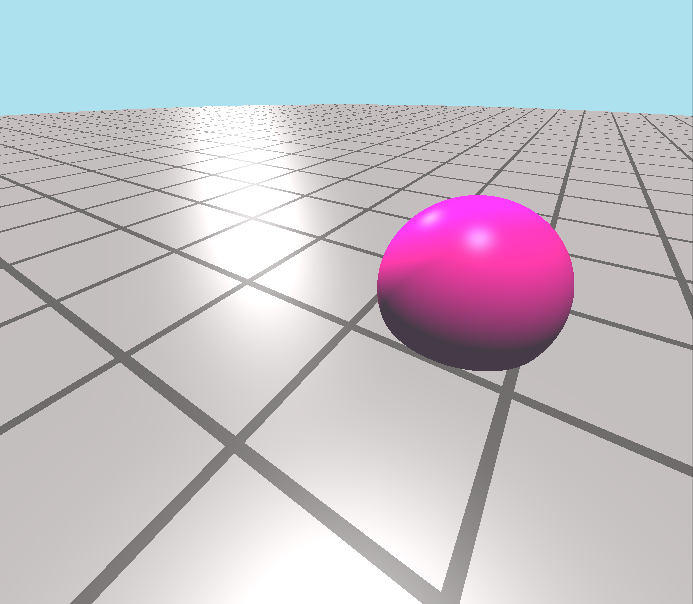
\includegraphics[width=0.9\textwidth]{Plantilla-TFG-master/img/compBP.png}
        \caption{Blinn-Phong}
     \end{minipage}
     \caption{Zonas brillantes en modelos de Blinn y Blinn-Phong}
     \label{fig:difBlinn}
\end{figure}

\begin{definicion}[Modelo de Blinn-Phong]
    En el contexto de la \autoref{def:blinn}, la radiancia percibida en el punto $p\in\R^3$ desde la dirección $v\in\R^3$ con $\Vert v \Vert = 1$ según el modelo de Blinn-Phong viene dada por
    \begin{equation*}
        L(p,v) = L_A+L_E+ \sum_{i=0}^n S_i \Bigg[ k_aR_A + \Max(0,l_i\cdot N_p) \left( k_dR_D + k_eR_E\cdot \left(N_p\cdot \frac{l_i + v}{\Vert l_i + v\Vert} \right)^{\alpha} \right) \Bigg].
    \end{equation*}
\end{definicion}

Ya podemos darle forma a las funciones \texttt{DibujarSuperficie} y \texttt{DibujarFondo} usadas en la \autoref{a:spheretracing}, suponiendo que pasamos como \textit{uniforms} los parámetros del material y los valores $l_i$ y $S_i$ para cada $i\in \{1,\dots, n\}$.
\begin{figure}[ht!]
    \centering
    
       \begin{algorithm}[H]
            \caption{DibujarSupercicie}
                \KwData{punto $p$, dirección del rayo $v$, distancia $\phi(p)$}
                \KwResult{terna RGB con la radiancia percibida en el punto $p$}
                $L \gets L_A$ \Comment{Radiancia final}
                \For{$i \in \{1,\dots, n\}$} {

                    
                    $h \gets normalizar(L_i - v)$ \Comment{Observador en dirección opuesta a la del rayo}
                    
                    $N_p \gets$ CalcularNormal$(p)$
                    
                    $NLi \gets \Max(0,\ N_p\cdot l_i)$
                    
                    $NH \gets \Max(0,\ N_p \cdot h)$\newline

                    $f_{ra} = R_A$
                    
                    $f_{rd} = NLi\cdot R_D$
                    
                    $f_{re} = NLi \cdot R_E \cdot NH^{\alpha}$\newline

                    $L \gets L + S_i\cdot (f_{ra} + f_{rd} + f_{re})$
                }

                \Return{$L$}
        \end{algorithm}
    \begin{algorithm}[H]
            \caption{DibujarFondo}
                \KwResult{terna RGB con el color de fondo de la escena}
                \Return{$L_A$}
        \end{algorithm}

        \caption{Implementación de las funciones \texttt{DibujarSuperficie} y \texttt{DibujarFondo}}
\end{figure}

Solo queda un asunto por tratar. A la vista de la expresión de $f_r$ \eqref{eq:fr} y del código anterior, somos capaces de calcular todos los valores a excepción de uno, el del vector normal. En la siguiente sección veremos presentamos una técnica para calcularlo de forma aproximada. 

\subsubsection{Cálculo del vector normal}
En cualquier modelo de iluminación el acceso al vector normal es indispensable. Cuando se trabaja con mallas de polígonos el vector normal viene dado para cada vértice, pero este no es nuestro caso. En su lugar nosotros usaremos el gradiente de la función distancia con signo para obtenerlo \cite{harvard}.
\begin{proposicion}\label{p:gradient_perp}
  Sea $\phi\colon \R^3\to \R$ diferenciable. Entonces $\nabla\phi$ es perpendicular a $S_\phi$.
\end{proposicion}
\begin{proof}
  Sea $s\in S_\phi$ arbitrario. Tomamos una curva parametrizada:
  \begin{align*}
    \alpha \colon [0,1] & \to S_\phi,\\
    t                   & \mapsto \left(x(t), y(t), z(t) \right),
  \end{align*}
  cumpliendo $\alpha(t_0)=s$ para algún $t_0\in [0,1]$. Veamos que $\nabla\phi(s) \perp \alpha$. Como $ \alpha(t)\subset S_\phi$ la evaluación de $\phi$ en cualquier punto de la curva será cero, y por tanto
  \begin{equation*}
      \frac{d}{dt}\phi(\alpha(t)) = 0.
  \end{equation*}
  Aplicando la regla de la cadena obtenemos
  \begin{equation*}
       \frac{d\phi \circ \alpha}{dt} = \frac{\partial{\phi}}{\partial{x}}\bigg\rvert_s \frac{dx}{dt}\bigg\rvert_{t_0} + \frac{\partial{\phi}}{\partial{y}}\bigg\rvert_s\frac{dy}{dt}\bigg\rvert_{t_0} + \frac{\partial{\phi}}{\partial{z}}\bigg\rvert_s\frac{dz}{dt}\bigg\rvert_{t_0} = \nabla \phi (s) \cdot \frac{d\alpha}{dt}\bigg\rvert_{t_0} = 0.
  \end{equation*}
    Por tanto $\nabla\phi(s)$ es perpendicular al vector tangente de $\alpha$ en $s$, que a su vez está contenido en el plano tangente de $S_\phi$ en $s$, luego $\nabla\phi(s) \perp S_\phi$.
\end{proof}

Hemos visto que calcular el vector normal en cualquier punto equivale a calcular $\nabla\phi$ y que este existe en casi todo punto de $S_{\phi}$ por el \autoref{teo:diff}, pero esto no significa que podamos o debamos obtenerlo de forma analítica. Si bien en muchos casos sería posible hacerlo de forma analítica, esto podría tener asociado un coste computacional que no podemos asumir. Existen varios métodos numéricos para aproximar el gradiente de una función. Uno de los más triviales es el de las diferencias centrales, basado en aproximar el límite de la \autoref{def:parcial} tomando un valor pequeño para $h$. Necesitaríamos entonces realizar seis evaluaciones de $\phi$ para obtener el gradiente, dos por cada parcial. Nosotros usaremos el \textbf{método del tetraedro} \cite{article:tetra}, que sin ser el más preciso,  produce buenos resultados y es rápido, haciendo uso únicamente de cuatro evaluaciones de $\phi$ en la dirección de los vértices de un tetraedro:


\begin{equation*}
    k_0 = (1,-1,-1),\quad k_1 = (-1,-1,1),\quad k_2=(-1,1,-1),\quad k_3=(1,1,1).
\end{equation*}

\begin{proposicion}[Método del tetraedro]
  Dado $p\in S_\phi$, una aproximación de su vector normal $N_p$ se obtiene normalizando el vector
  \begin{equation*}
    \hat{N_p} = \sum_{i=0}^3 k_i\cdot f(p + hk_i)\quad \text{, donde } h\approx 0.
  \end{equation*}
\end{proposicion}

\begin{proof}
  Por la proposición \autoref{p:gradient_perp}, basta comprobar que $\hat{N}$ es colineal a $\nabla \phi(p)$.
  \begin{align*}
    \hat{N} & = \sum_{i=0}^3 k_i\cdot f(p + hk_i) = \sum_{i=0}^3 k_i\cdot f(p + hk_i) - k_i\cdot f(p) = \sum_{i=0}^3 k_i\cdot \left[ f(p+hk_i) - f(p)\right]\\ &= h\sum_{i=0}^3 k_i \nabla_{k_i}f(x)
    = h\sum_{i=0}^3 k_i \cdot \left( k_i \cdot \nabla f(p)\right) = h\sum_{i=0}^3 (k_i\cdot k_i) \nabla f(p) = h\sum_{i=0}^3 \nabla f(p) = 4h\nabla f(p).
  \end{align*}
  Hemos usado que $\sum_{i=0}^3 k_i = (0,0,0)$, $\sum_{i=0}^3 k_i\cdot k_i = (1,1,1)$ y que el producto escalar es un operador lineal.
\end{proof}

\subsection{Sombras}
Los resultados obtenidos en la \autoref{fig:difBlinn} presentan ciertas carencias, siendo la más flagrante la ausencia de sombras arrojadas, que no son consideradas en el modelo de Blinn-Phong. Afortunadamente el uso de las SDFs nos hará la obtención de la información necesaria para añadir sombras a nuestra escena muy sencilla. Para saber si un punto $p\in\R^3$ recibe luz de una $i$-ésima fuente de luz bastará comprobar si hay algún obstáculo entre dicha fuente y el punto. Para hacer esta comprobación usaremos de nuevo \textit{spheretracing}, pero en esta ocasión desde el punto hacia la fuente de luz. Si se detecta alguna intersección significará que el punto $p$ no recibe luz de la fuente y por tanto $L_R(p,v,l_i) = 0,\ \forall v\in \R^3$. Podemos modificar \texttt{DibujarSuperficie} como se muestra en la \autoref{fig:sombras1} para añadir este comprobación.\newline

\begin{algorithm}[H]
        \caption{DibujarSupercicie}
            \KwData{punto $p$, dirección del rayo $v$, distancia $\phi(p)$}
            \KwResult{terna RGB con la radiancia percibida en el punto $p$}
            $L \gets L_A + L_E$ \Comment{Radiancia final}
            \For{$i \in \{1,\dots, n\}$} {

                \Comment{ ··· }
                $sombras \gets CalcularSombras(p, l_i)$

                $L \gets L + S_i\cdot (f_{ra} + f_{rd} + f_{re})\cdot sombras$
            }

            \Return{$L$}
    \end{algorithm}
\begin{figure}[ht!]
    \centering
    \begin{minipage}{0.50\textwidth}
   \begin{algorithm}[H]
            \caption{CalcularSombras}
                \KwData{punto $p_0$, dirección de luz $l_i$}
                \KwResult{factor de sombra en $p_0$ en el rango $[0,1]$}
                 $d \gets \delta$ \Comment{distancia actual}
                
                \For{i $\in$ MAX\_ITERACIONES} {
                    $p \gets p_o + d \cdot v$
                    
                    $sdf \gets \phi(p)$
                    
                    \If{sdf $< \varepsilon$}{
                       \Return{0};
                    }
            
                    $d \gets d + sdf$

                    \If{d > MAX\_DISTANCIA}{
                        \Return{1}
                    }
                }

                \Return{1}
        \end{algorithm}
    \end{minipage}%
    \hfill
    \begin{minipage}{0.48\textwidth}
        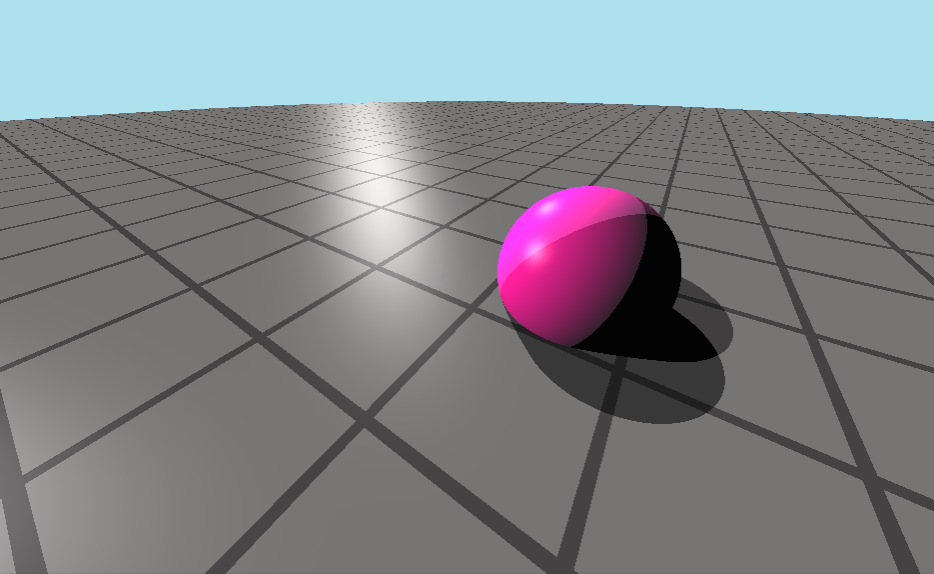
\includegraphics[width=\textwidth]{shadowSimple.png}
    \end{minipage}
    \caption{Cálculo básico de sombras}
    \label{fig:sombras1}
\end{figure}


Realizamos las siguientes apreciaciones respecto al método \texttt{CalcularSombras} propuesto:
\begin{itemize}
    \item Dado que estamos trabajando con luces direccionales situadas a distancia infinita solo podemos hacer \textit{spheretracing} desde $p$ en dirección a la fuente, a pesar de que lo intuitivo sería hacerlo desde el foco de luz hacia el punto.
    \item A diferencia del algoritmo propuesto en \autoref{a:spheretracing} no podemos inicializar $d=0$, ya que entonces se detectaría una intersección en el mismo punto $p$.
\end{itemize}

Estudiando los resultados obtenidos vemos que al añadir sombras obtenemos una imagen mucho más cohesiva y otorgamos a la esfera mayor presencia en la escena. Sin embargo también podremos apreciar que las sombras que genera este método son muy planas y duras. Realmente ahora mismo no tenemos control alguno sobre esto, ya que según nuestra implementación un punto o está totalmente en sombra o totalmente iluminado. Esto no siempre es así en el mundo real, donde podemos encontrar que no toda la región sombreada sea igual de oscura o el borde esté más o menos difuminado en función de las propiedades de la fuente. Podemos simular estos fenómenos de forma muy sencilla usando información de la que ya que disponemos en el algoritmo de \textit{spheretracing}. En particular:
\begin{itemize}
    \item Haremos que cuanto más cerca se encuentre el punto del obstáculo que le hace sombra menos luz reciba. Por tanto la intensidad de la sombra será proporcional a la evaluación de la SDF en el punto actual del rayo:
    \begin{equation*}
        sombra \propto sdf.
    \end{equation*}
    \item Cuando un punto sea alcanzado por la luz pero haya estado muy cerca de ser obstruido dejaremos que refleje solo una fracción de la luz total. Esta cantidad deberá ser mayor cuanto menos haya faltado para perder la intersección, creando un difuminado en el borde:
    \begin{equation*}
        sombra \propto \frac{1}{d}.
    \end{equation*}
\end{itemize}

Esta nueva versión de \texttt{CalcularSombras} se encuentra descrita en la \autoref{fig:sombras2}. En ella se ha añadido un parámetro $k\in \R_0^+$ para controlar la intensidad del efecto de suavizado. En realidad este parámetro hace referencia al \textbf{tamaño de la fuente de luz}, en concreto a su inversa. Así, cuanto más pequeño sea este valor más grande será la fuente de luz, produciendo sombras más difusas. Por ejemplo, el Sol tendrá un valor pequeño para $k$, mientras que una bombilla lo tendría grande. A partir de ahora en nuestra escena de ejemplo fijamos $k=  1.5$ para la fuente de luz que apunta más hacia la cámara, que actuará como el Sol, y $k = 10$ para la otra, que actuará como una linterna.\newline

\begin{figure}[ht!]
    \centering
    \begin{minipage}{0.50\textwidth}
       \begin{algorithm}[H]
            \caption{CalcularSombras}
                \KwData{punto $p_0$, dirección de luz $l_i$, tamaño de luz $k$}
                \KwResult{factor de sombra en $p_0$ en el rango $[0,1]$}
                $sombra \gets 1$
                
                $d \gets \delta$ \Comment{distancia actual}
                
                \For{i $\in$ MAX\_ITERACIONES} {
                    $p \gets p_o + d \cdot v$
                    
                    $sdf \gets \phi(p)$
                    
                    \If{sdf $< \varepsilon$}{
                       \Return{0};
                    }
                    $sombra \gets \Min(sombra, k\cdot \frac{sdf}{d})$
                    
                    $d \gets d + sdf$

                    \If{d > MAX\_DISTANCIA}{
                        \Return{1}
                    }
                }

                \Return{1}
        \end{algorithm}
    \end{minipage}%
    \hfill
    \begin{minipage}{0.48\textwidth}
        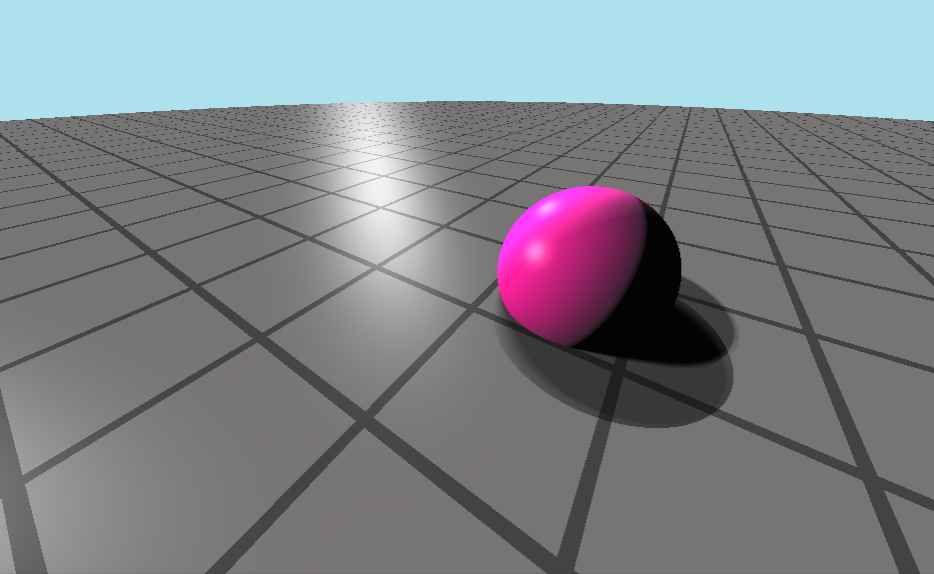
\includegraphics[width=\textwidth]{shadowSoftArtifact.png}
    \end{minipage}
    \caption{Cálculo de sombras suavizadas}
    \label{fig:sombras2}
\end{figure}

Si bien este método genera resultados más realistas en general, también puede generar ciertas imperfecciones en el borde de la sombra, como se puede apreciar en la \autoref{fig:artifactZoom}. Esto es debido a que en el proceso de \textit{spheretracing} podemos saltarnos una intersección que habría aportado más oscuridad que la que finalmente se ha encontrado, generando fugas de luz que siguen el patrón de los puntos en los que se evalúa la SDF. Hay varias formas de solventar esto, como la propuesta por Sebastian Aaltonen \cite{gdc} en la GDC de 2018. Su idea se basa en comprobar intersecciones también en los puntos que se estiman como los más cercanos a la superficie en cada iteración. Nosotros usaremos una técnica introducida por el usuario \texttt{nurof3n} \cite{shadertoy-sombras} en Shadertoy y estudiada posteriormente por Íñigo Quílez.\newline

\begin{figure}[ht!]
    \centering
    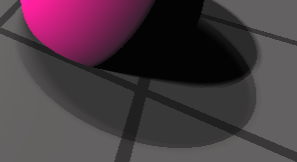
\includegraphics[width=0.7\textwidth]{Plantilla-TFG-master/img/shadowArtifactZoom.png}
    \caption{Detalle de las fugas de luz al calcular sombras}
    \label{fig:artifactZoom}
\end{figure}

La diferencia con nuestro método actual radica en que se permite que el rayo penetre un poco la superficie para detectar los puntos que casi no son alcanzados por un rayo de luz. Por tanto, ahora para cada punto se tiene en cuenta si casi ha sido alcanzado y si casi no ha sido alcanzado por un rayo de luz. Para permitir que el rayo entre en la geometría basta con modificar la condición de ruptura sobre $sdf$ a un número negativo, con la precaución de siempre sumar una cantidad positiva a $d$, pues de lo contrario el trazado del rayo retrocedería. Fijando este valor a $-1$ la variable $sombra$ tendrá un valor en el rango $[-1,1]$ al salir del bucle, pero aún queremos obtener un valor entre $[0,1]$ para representar la cantidad de luz que recibe el punto. Para remapear $sombra$ a este rango podemos usar la función \texttt{smoothstep(a,b,x)} de GLSL, que interpola $x$ suavemente entre $0$ y $1$ en relación con los límites $a$ y $b$. En particular la interpolación que se lleva a cabo es la de Hermite, haciendo que la transición entre distintos puntos de sombra no sea lineal y parezca más natural. Podemos ver el algoritmo final en la \autoref{fig:sombras3} y los resultados que consigue en la \autoref{fig:sombras4}.

\begin{figure}[ht!]
    \centering
    \includegraphics[width=0.3\textwidth]{Plantilla-TFG-master/img/smoothstep.png}
    \caption{Visualización de \texttt{smoothstep} \cite{smoothstep}}
    \label{fig:miss}
\end{figure}

\begin{figure}[ht!]
    \centering
   \begin{algorithm}[H]
        \caption{CalcularSombras}
            \KwData{punto $p_0$, dirección de luz $l_i$, tamaño de luz $k$}
            \KwResult{valor en el rango $[0,1]$ representando la cantidad de sombra recibida en $p_0$}
            $sombra \gets 1$
            
            $d \gets \delta$ \Comment{distancia actual}
            
            \For{i $\in$ MAX\_ITERACIONES} {
                $p \gets p_o + d \cdot v$
                
                $sombra \gets \Min(res, k\cdot \frac{sdf}{d})$
                
                $sdf \gets \phi(p)$

                $d \gets d + \vert sdf\vert$
                
                \If{$sombra < -1 $ \textbf{OR} $d > MAX\_DISTANCIA$}{
                   \textbf{break}
                } 
            }

            \Return{$smoothstep(-1,1,sombra)$}
    \end{algorithm}

    \caption{Cálculo de sombras suavizadas mejorado}
    \label{fig:sombras3}
\end{figure}

\begin{figure}[ht!]
    \centering
    \includegraphics[width=\textwidth]{Plantilla-TFG-master/img/shadowSoft.png}
    \caption{Resultado final del cálculo de sombras}
    \label{fig:sombras4}
\end{figure}



\subsection{Oclusión ambiental}
Al añadir sombras los objetos están mucho más integrados en la escena, pero todavía podemos conseguir un mayo grado de cohesión. En el estado actual de la escena aún hay puntos que no es convincente que reciban luz pero se encuentran totalmente iluminados. Un ejemplo son los puntos de intersección entre la esfera y el suelo. Uno esperaría que poca luz fuera capaz de alcanzar un espacio tan cóncavo, pues la propia geometría de la esfera y el suelo ocluirían la luz. Este fenómeno recibe el nombre de \textbf{oclusión ambiental}, y de nuevo gracias a los SDF nos resultará muy fácil y computacionalmente barato simularlo.\newline

Cuando se trabaja con geometría de polígonos, una de las técnicas más comunes es la oclusión ambiental del espacio de pantalla, o SSAO por sus siglas en inglés. En su versión más básica esta solución usa la información del fotograma actual para consultar por cada píxel el \textif{buffer} de profundidad o \textit{deph buffer} de los píxeles cercanos. Con esta información realiza una aproximación de las características de la geometría en ese entorno y deduce la cantidad de luz que debería poder pasar. El principal problema de esta y otras técnicas basadas en el espacio de pantalla es que al no usar la información real de la geometría, los resultados obtenidos varían según la orientación de la cámara, posición relativa de los objetos en pantalla, etc. Otro método basado en espacio de pantalla que pone de manifiesto este problema es el de los reflejos de espacio de pantalla o SSR, que suele ser usado para simular reflejos como los del agua o espejos en videojuegos. Al usar el mismo principio que SSAO, solo podrá reflejar correctamente los píxeles que estén dibujados en pantalla. Esta limitación hace que cuando un objeto ocluye a otro este no se puede reflejar correctamente y se generen reflejos erróneos como se muestra en la \autoref{fig:ssrVS}, o que si un objeto no aparece en pantalla directamente no sea reflejado, como se representa en la \autoref{fig:ssrEsquema}.

\begin{figure}[!h]
     \begin{minipage}[c]{0.49\linewidth}
        \centering
        \includegraphics[width=0.98\textwidth]{Plantilla-TFG-master/img/ssr_on.png}
        \caption{SSR}
     \end{minipage}
     \begin{minipage}[c]{0.49\linewidth}
        \centering
        \includegraphics[width=0.98\textwidth]{Plantilla-TFG-master/img/ssr_off.png}
        \caption{\textit{Raytracing}}
     \end{minipage}
     \caption{Videojuego Ratchet \& Clank: Una dimensión aparte usando SSR y \textit{raytracing} \cite{ratchet}}
     \label{fig:ssrVS}
\end{figure}

\begin{figure}[!h]
     \begin{minipage}[c]{0.49\linewidth}
        \centering
        \includegraphics[width=0.9\textwidth]{Plantilla-TFG-master/img/ssr2.png}
        \caption{Reflejo detectado}
     \end{minipage}
     \begin{minipage}[c]{0.49\linewidth}
        \centering
        \includegraphics[width=0.9\textwidth]{Plantilla-TFG-master/img/ssr3.png}
        \caption{Reflejo no detectado}
     \end{minipage}
     \caption{Reflejos en agua con SSR}
     \label{fig:ssrEsquema}
\end{figure}

La solución a estos problemas cuando se trabaja con vértices es el uso de técnicas más avanzadas y computacionalmente costosas como el \textit{raytracing}. La buena noticia es que al estar usando SDFs nosotros podremos usar la información real de la geometría de nuestra escena. Obtendremos por tanto información más precisa, y además de forma muy barata, ya que requeriremos de muchas menos evaluaciones del SDF que el algoritmo de \textit{spheretracing}. La técnica que vamos a usar fue ideada por Alex Evans en 2006 \cite{ao}, y se conoce como \textbf{oclusión ambiental muestreada por la normal}.\newline

El método se basa en dado un punto $p\in S_{\phi}$ evaluar el SDF en varios puntos del vector normal $N_p$ a distancias $d_i$ de $p$ para obtener la información de la geometría cercana. Si en el entorno de $p$ hay geometría que le esté obstruyendo la llegada de luz, en alguna de estas evaluaciones se obtendrá un valor menor que $d_i$, mientras que de lo contrario uno esperaría que
\begin{equation*}
    \phi(p + d_i N_p) = d_i,
\end{equation*}
ya que eso significaría que el punto más cercano a $p$ de $S_{\phi}$ es el propio $p$. Así, si hacemos $M$ evaluaciones igualmente espaciadas a lo largo de $N_p$, consideraremos que el punto $p$ no está ocluido si
\begin{equation*}
    \sum_{i=1}^M \phi\Big(p + \frac{i}{M} N_p\Big) - \sum_{i=1}^M \frac{i}{M} = 0.
\end{equation*}
\begin{figure}[ht!]
    \centering
    \includegraphics[width=\textwidth]{Plantilla-TFG-master/img/diagramaAO.png}
    \caption{Cálculo de oclusión ambiental muestreada por la normal}
    \label{fig:sombras4}
\end{figure}
Cuanto mayor sea este valor (no puede ser menor que $0$ por definición de SDF) menos luz será capaz de alcanzar $p$. Así, podemos representar la cantidad de luz ocluida como
\begin{equation*}
    \sum_{i=1}^M \frac{1}{2^i}\cdot \left(\frac{i}{M} - \phi\Big(p + \frac{i}{M} N_p\Big)\right)\in [0,1].
\end{equation*}
El hecho de que esté valor esté acotado en $[0,1]$ viene de que suponemos que $\Vert N_p\Vert = 1$, de forma que
\begin{equation*}
    \phi\left(p + \frac{i}{M} N_p\right) \le 1,
\end{equation*}
ya que siempre habrá algún punto a lo largo de $N_p$ que esté a una unidad o menos de distancia de $p$: él mismo. Por otro lado, hemos usado la exponencial para dar más peso sobre el resultado final a aquellos puntos más cercanos a $p$.\newline

Con esto ya podemos obtener la nueva versión del método \texttt{DibujarSuperficie} que tiene en cuenta la oclusión ambiental descrita en la \autoref{fig:dibujarAO}. En ella hemos introducido una pequeña optimización \cite{ao_opt} cambiando el índice del bucle para no tener que calcular una división en cada iteración. Otra posible optimización sería sustituir la potencia por un un flotante que fuéramos multiplicando por un factor menor que $1$ en cada iteración. Finalmente, podemos apreciar los resultados obtenidos en la \autoref{fig:resAO}, donde para valores tan pequeños de $M$ como $2$ o $4$ ya conseguimos resultados más que convincentes.

% donde hemos usado la exponencial para asegurar que $ao\in [0,1]$, que cuando no haya oclusión obtengamos $ao=1$ y que el resultado tenga un aspecto más natural. Además $k$ controlará la intensidad del efecto. Sin embargo preferiremos ganar algo de eficiencia simulando el comportamiento de la exponencial con una constante que iremos multiplicando por sí misma en cada iteración. Así, la nueva versión del método \texttt{DibujarSuperficie} será el descrito en la \autoref{fig:dibujarAO}.

\begin{figure}
    \centering
        
    \begin{algorithm}[H]
        \caption{DibujarSupercicie}
            \KwData{punto $p$, dirección del rayo $v$, distancia $\phi(p)$}
            $L \gets L_A + L_E$ \Comment{Radiancia final}
            \For{$i \in \{1,\dots, n\}$} {
    
                
                \Comment{ ··· }
                $N_p \gets CalcularNormal(p)$
                
                $sombras \gets CalcularSombras(p, l_i)$
                
                $ao \gets CalcularAO(p, N_p)$
    
                $L \gets L + S_i\cdot (f_{ra} + f_{rd} + f_{re})\cdot sombras \cdot ao$
            }
    
            \Return{$L$}
    \end{algorithm}
    
    \begin{algorithm}[H]
        \caption{CalcularAO}
            \KwData{punto $p$, vector normal $N_p$}
            \KwResult{$ao \in [0,1]$}
            $ao \gets 1$
                    
            $increment \gets \nicefrac{1}{M}$
            
            $i\gets increment$
        
            \While{$i<1$}{
                $sdf \gets \phi(p + iN_p)$
                
                $ao \gets ao - 2^{-iM}\cdot (i-sdf)$
    
                $i\gets i+increment$
            }
                
            \Return{$ao$}
    \end{algorithm}
    
    \caption{Cálculo de oclusión ambiental}
    \label{fig:dibujarAO}
\end{figure}


\begin{figure}[!h]
     \begin{minipage}[c]{0.49\linewidth}
        \centering
        \includegraphics[width=0.98\textwidth]{Plantilla-TFG-master/img/ao2.png}
        \caption{$M=2$}
     \end{minipage}
     \begin{minipage}[c]{0.49\linewidth}
        \centering
        \includegraphics[width=0.98\textwidth]{Plantilla-TFG-master/img/ao4.png}
        \caption{$M=4$}
     \end{minipage}
     \caption{Resultado del cálculo de oclusión ambiental}
     \label{fig:resAO}
\end{figure}

\section{\textit{Antialiasing}}\label{sec:aa}
Vamos a introducir una última mejora en la forma en la que generamos la imagen. Un defecto típico en computación gráfica es el conocido como \textbf{\textit{aliasing}}. Este se caracteriza por la presencia de dientes de sierra en lineas curvas o diagonales, y en nuestro caso se puede apreciar muy fácilmente en los bordes del cubo y en la cuadrícula del suelo en la distancia (\autoref{subfig:noAA}). En el mercado actual existen multitud de alternativas como solución a este problema. Algunos ejemplos son FXAA, basado en espacio de pantalla, o SSAA y MSAA, que usan la técnica del \textbf{supermuestreo} o \textbf{\textit{supersampling}} junto con filtros de suavizado. Nosotros implementaremos una versión de SSAA (\textit{Supersampling Anti-Aliasing}), pero antes debemos entender por qué aparece el problema del \textit{aliasing} en primer lugar. \newline

Toda pantalla tiene resolución finita, y por tanto la definición con la que puede mostrar la información es limitada. Al realizar la proyección sobre la pantalla puede ocurrir que una primitiva no ocupe un píxel completo, y como cada píxel solo puede mostrar un único color hay que elegir algún criterio para determinar qué hacer en esos casos. El más común es considerar que el píxel pertenece a la primitiva si su proyección cubre el centro del píxel. En nuestro caso esto se traducía en trazar el rayo a través del centro del píxel en el algoritmo de \textit{spheretracing}. Al hacer esta aproximación es cuando aparecen los dientes de sierra, pues a no ser que se trate de una línea totalmente vertical u horizontal, es como si intentásemos construir una rampa con escalones.\newline

Lo cierto es que no podemos hacer desaparecer este problema, pues es algo intrínseco de la naturaleza discreta de las pantallas y los sistemas de muestreo. En nuestro caso esto último se traduce en que no podemos trazar infinitos rayos. No obstante, lo que sí podemos hacer es tratar de disimularlo. En lugar de tomar una decisión binaria de si un píxel debe ser de un color u otro podemos intentar tener en cuenta la aportación de otras primitivas que estén cercanas dentro del píxel aunque no ocupen su centro. Una primera idea podría ser que una vez asignado un color a un píxel se hiciera la media con sus píxeles vecinos para así generar una transición suave entre ellos. Sin embargo este acercamiento presenta dos grandes inconvenientes:
\begin{itemize}
    \item Estaríamos perdiendo parte de la información original, y por ende, haciendo la imagen más borrosa.
    \item El responsable de asignar el color de cada píxel es una instancia del \textit{fragment shader}, y como ya comentamos, los \textit{shaders} son programas independientes y no tienen información sobre el resto de instancias. Por tanto este método sería de postprocesado, es decir, sería ejecutado una vez hubiera sido generada la imagen.
    
\end{itemize}

De esto podemos sacar la conclusión de que la solución debe ser local a cada píxel, y de ser posible que no conlleve la pérdida de información. La opción de hacer una media entre varias muestras de píxeles sigue pareciendo razonable, lo que nos lleva a la idea detrás de SSAA: tomar más muestras dentro de cada píxel. Para ello, tendremos que trazar rayos por más puntos dentro del píxel, esto es, dibujar la imagen con mayor resolución, de donde viene el nombre de supermuestreo. El patrón en el que tomamos las nuevas muestras es de nuestra elección. En la \autoref{fig:patrones} se muestran algunos patrones comunes, de los cuales optaremos por el uniforme por su sencillez y porque proporciona resultados bastante buenos en general. El número de evaluaciones también está a nuestra elección, pero no hay que olvidar el factor del rendimiento, ya que usando este patrón el número de rayos crece exponencialmente por cada nuevo nivel adicional de precisión.
\newline

\begin{figure}[htbp]
    \centering
    \begin{subfigure}[b]{0.25\textwidth}
        \centering
        \includegraphics[width=\textwidth]{Plantilla-TFG-master/img/aa1.png}
        \caption{Uniforme}
    \end{subfigure}
    \hfill
    \begin{subfigure}[b]{0.25\textwidth}
        \centering
        \includegraphics[width=\textwidth]{Plantilla-TFG-master/img/aa2.png}
        \caption{Rejilla girada}
    \end{subfigure}
    \hfill
    \begin{subfigure}[b]{0.25\textwidth}
        \centering
        \includegraphics[width=\textwidth]{Plantilla-TFG-master/img/aa3.png}
        \caption{Aleatorio}
    \end{subfigure}
    
    \medskip
    
    \begin{subfigure}[b]{0.25\textwidth}
        \centering
        \includegraphics[width=\textwidth]{Plantilla-TFG-master/img/aa4.png}
        \caption{\textit{Quasi-Monte Carlo}}
    \end{subfigure}
    \hfill
    \begin{subfigure}[b]{0.25\textwidth}
        \centering
        \includegraphics[width=\textwidth]{Plantilla-TFG-master/img/aa5.png}
        \caption{HRAA}
    \end{subfigure}
    \hfill
    \begin{subfigure}[b]{0.25\textwidth}
        \centering
        \includegraphics[width=\textwidth]{Plantilla-TFG-master/img/aa6.png}
        \caption{\textit{Flipquad}}
    \end{subfigure}
    \caption{Patrones de supermuestreo \cite{supersamp}}
    \label{fig:patrones}
\end{figure}

Modificar por dónde pasan los rayos dentro de cada píxel equivale a cambiar cómo calculamos los \texttt{uv}. Llamaremos a partir de ahora $AA$ al factor de escalado de la imagen, de forma que por cada píxel haremos pasar $4^{AA-1}$ rayos. Para hallar los nuevos puntos de muestra bastará con subdividir el píxel en $AA^2$ cuadrantes y quedarnos con el centro de cada uno. Si recordamos que $v_{frag}$ devuelve las coordenadas del centro del píxel, que el ancho y alto del píxel es una unidad, y que tenemos que hacer $AA$ subdivisiones en cada eje, es evidente que podemos obtener los nuevos puntos de muestra desplazando el origen usual del píxel la cantidad
\begin{equation*}
    offset_{m,n} = (m+\nicefrac{1}{2},n+\nicefrac{1}{2}))\cdot subdivision - \left( \frac{lado}{2}, \frac{lado}{2}\right) = \frac{ (m+\nicefrac{1}{2},n+\nicefrac{1}{2}))}{AA} - \left( \frac{1}{2}, \frac{1}{2}\right),
\end{equation*}
donde $m,n\in \{0,\dots, AA-1\}$.\newline
\begin{figure}[!h]
    \centering
    \begin{subfigure}[b]{0.4\textwidth}
        \centering
        \includegraphics[width=\textwidth]{Plantilla-TFG-master/img/grid1.png}
        \caption{$AA = 1$}
    \end{subfigure}
    \hspace{15pt}
    \begin{subfigure}[b]{0.4\textwidth}
        \centering
        \includegraphics[width=\textwidth]{Plantilla-TFG-master/img/grid2.png}
        \caption{$AA = 2$}
    \end{subfigure}
    \hfill
     \caption{\textit{Antialiasing} para diferentes valores de $AA$}
\end{figure}

Para trasladar esto a nuestro \textit{fragment shader} tan solo habrá que realizar un doble bucle e ir sumando el color obtenido por \textit{spheretracing} en una variable que luego ponderaremos por el número total de muestras, $AA^2$. La nueva versión del \textit{fragment shader} se describe en la \autoref{fig:divPixel}.

\begin{figure}[ht!]
    \centering
    \begin{minipage}{0.69\textwidth}
      \begin{algorithm}[H]
            \caption{Fragment Shader}
            \KwData{coordenadas de dispositivo $v_{frag}$ del píxel actual}
            \KwResult{color del píxel actual como terna RGBA $v_{col}$}
            $c_0 \gets $ posición de cámara en función de la entrada del ratón

            $l\gets $ punto de atención elegido por el usuario
            
            $color\gets (0,0,0)$
            
            \For{$m \in \{0,\dots, AA-1\}$}{
            \For{$n \in \{0,\dots, AA-1\}$}{
                $offset \gets \frac{(m,n)}{AA} - (0.25, 0.25)$\\[8pt]
                
                $uv \gets 2\cdot \frac{(v_{frag}+offset)- 0.5\cdot u\_resolution.xy}{u\_resolution.y}$\\[8pt]

                $r_d \gets (f_1\ \vert \ f_2\ \vert \ f_3)\cdot normalizar((uv_x, uv_y,-1))$\\[5pt]

                $color \gets color + spheretracing(c_0, r_d)$
                }
            }

            $color \gets color / AA^2$
            
            $v_{col} \gets (color_x, color_y, color_z, 1)$
        \end{algorithm}
    \end{minipage}%
    \hfill
    \begin{minipage}{0.31\textwidth}
        \includegraphics[width=\textwidth]{buclePixels.png}
    \end{minipage}
    \caption{Cuerpo del método \texttt{main} del \textit{fragment shader}}
    \label{fig:divPixel}
\end{figure}

Es evidente que $AA=1$ equivale a no aplicar \textit{antialiasing}, pero tendrá el efecto de desplazar la imagen medio píxel hacia abajo y a la izquierda, pues el único de cada píxel pasará por su esquina inferior. Por tanto, aunque no sea totalmente necesario, se puede añadir una comprobación para calcular los $uv$ como hacíamos originalmente en este caso. En la \autoref{fig:resAA} podemos ver que la pérdida de rendimiento no es en vano y obtenemos una imagen mucho más suave que la original. Sin embargo, no conviene tomar un valor de $AA$ mayor que $3$, pues generará mucha sobrecarga y la mejora no es muy apreciable. Finalmente y para concluir la sección, en el \autoref{ap:comparacionEscenas} podemos ver la construcción que hemos hecho de la escena paso a paso, viendo el efecto que ha tenido en el aspecto final cada técnica que hemos ido añadiendo.

\begin{figure}[htbp]
    \centering
    \begin{subfigure}[b]{0.3\textwidth}
        \centering
        \includegraphics[width=\textwidth]{Plantilla-TFG-master/img/aa1_zoom.png}
        \caption{Detalle con $AA = 1$}
        \label{subfig:noAA}
    \end{subfigure}
    \hfill
    \begin{subfigure}[b]{0.3\textwidth}
        \centering
        \includegraphics[width=\textwidth]{Plantilla-TFG-master/img/aa2_zoom.png}
        \caption{Detalle con $AA = 2$}
    \end{subfigure}
    \hfill
    \begin{subfigure}[b]{0.3\textwidth}
        \centering
        \includegraphics[width=\textwidth]{Plantilla-TFG-master/img/aa3_zoom.png}
        \caption{Detalle con $AA = 3$}
    \end{subfigure}

    \medskip
    
    \begin{subfigure}[b]{\textwidth}
        \centering
        \includegraphics[width=\textwidth]{Plantilla-TFG-master/img/escena9_AA3.png}
        \caption{Escena completa con $AA=3$}
    \end{subfigure}
    
    \caption{Resultados de añadir \textit{antialiasing}}
    \label{fig:resAA}
\end{figure}






% !TeX root = ../libro.tex
% !TeX encoding = utf8

\chapter{Desarrollo e implementación}
En esta sección veremos cómo se han usado las técnicas y conceptos presentados para la realización de una aplicación web que permita al usuario crear e interactuar superficies a través de SDFs, ecuaciones implícitas y paramétricas. El motivo de desarrollar una aplicación web es que sea accesible al mayor número de usuarios y de la forma más cómoda posible. Se ha decidido usar \href{https://es.reactjs.org/}{React} para esta tarea, una biblioteca de JavaScript (y TypeScript) para interfaces de usuario. Es una librerçia muy popular, y por tanto muy bien documentada y con muchos paquetes de la comunidad disponibles. Las principales características de React son:
\begin{itemize}
    \item Utiliza la \textbf{extensión de sintaxis} JSX, la cual permite escribir código JavaScript como si se tratase de HTML o XML. Se pueden usar expresiones JSX dentro de bucles \texttt{for} o entornos condicionales \texttt{if}, y dentro de ellas se pueden agregar expresiones JS entre corchetes. 
    \item Se basa en \textbf{componentes autocontenidos y reutilizables}. La forma más común actualmente de declarar componentes es a través de funciones que reciben argumentos, o \texttt{props}, y devuelven una expresión JSX. Todos los componentes reciben el parámetro \texttt{children} por defecto, conteniendo la expresión JSX de los componentes que se encuentren entre las etiquetas de apertura y cierre del componente. El flujo de datos es unidireccional del componente padre a sus hijos.
    \item Utiliza un \textbf{DOM virtual} para solo actualizar los componentes cuyo estado o \texttt{props} han cambiado. En componentes funcionales, la manera de indicar variables que desencadenen un re-renderizado al ser modificadas es a través de \texttt{hooks}. En general, estos son funciones de JS que permiten crear y acceder al estado y ciclos de vida de React. Los principales son \texttt{useState}, usado para declarar una variable junto con su \textit{setter}, y \texttt{useEffect}, que permite ejecutar código cuando se actualice el componente. Si solo se quiere reaccionar a cambios de ciertos \textit{hooks} se puede indicar en las dependencias.
\end{itemize}

Un ejemplo de uso básico de JSX, componentes funcionales y manejo de estado sería el siguiente:
\begin{lstlisting}
function Tarjeta(props) {
  return (
    <div>
        {props.children}
        {props.nombre}
    </div>
  );
}

function Main() {
    const [miNombre, setMiNombre] = React.useState("Daniel");

    useEffect(()=>{
        console.log("Solo me ejecuto una vez al inicio");
    }, []);
    
    useEffect(()=>{
        console.log("Has cambiado el nombre");
    }, [miNombre]);
    
  return (
    <TarjetaNombre nombre={miNombre}>
      <h1>Hola, mi nombre es</h1>
    </TarjetaNombre>
  );
}
\end{lstlisting}

Las principales ventajas que aporta son:
\begin{itemize}
    \item La aplicación puede ser ejecutada en cualquier navegador, haciendo que sea mucho más accesible,
    \item Está basada en componentes modulares, lo que la hace escalable. Además. debido a su popularidad, hay una infinidad de librerías de terceros a nuestra disposición, ya sea específicas de React o de JavaScript.
\end{itemize}

% Un aspecto fundamental a lo largo de todo el desarrollo será el del rendimiento ya que las aplicaciones web solo tienen a su disposición una hebra de ejecución (la de interfaz de usuario), haciendo de cuello de botella para el resto de cálculos.\newline

La aplicación consta de tres componentes principales. Dos de ellos son con los que interactúa el usuario, uno en la que se le permite crear primitivas introduciendo directamente una SDF, ecuaciones implícitas o paramétricas, y otro que contiene un editor de nodos en forma de árbol para aplicar operaciones sobre las primitivas creadas y guardar los resultados obtenidos. El último componente actúa como gestor de almecenamiento y estado de la aplicación. A continuación estudiamos cada componente por separado describiendo los subcomponentes que la conforman y cómo estos interaccionan entre sí.


\section{Editor de nodos}
Este componente se base en \href{https://github.com/wbkd/react-flow}{React Flow}, un paquete muy completo que permite la implementación de diagramas interactivos basados en nodos. Cada nodo tendrá cierto número de puertos de entrada (solo permite la conexión con un nodo) y uno de salida (permite conectarse a varios nodos). Se nos permite declarar tipos de nodos según nuestras necesidades. Nosotros usaremos dos categorías principales de nodos.\newline

El \textbf{nodo de primitiva} es el más sencillo, y permite seleccionar una primitiva entre las guardadas para ser conectada a uno o varios nodos de operaciones.\newline

Los \textbf{nodos de operaciones} implementan las operaciones explicadas en la \autoref{sec:operaciones} y las aplican a las primitivas que reciben por sus puertos de entrada. A su vez hay cuatro tipos diferentes de estos nodos, uno por cada tipo de operación. Los nodos de operaciones de transformación, deformación y repetición tienen un único puerto de entrada, pues son operadores unarios. El nodo booleano sin embargo es capaz de recibir un número arbitrario de primitivas, ya que aunque los operadores booleanos son binarios, si se quiere realizar una misma operación de forma reiterada sobre varias primitivas puede ser muy tedioso. Así, si un nodo booleano recibe las primitivas $A_i$ con $i=1,\dots, n$, irá aplicando la operación de forma sucesiva sobre el resultado anterior según el orden de conexión. Por ejemplo, para la unión tendríamos
\begin{equation*}
    \bigcup_{i=0}^n A_i = A_n\bigcup (A_{n-1} \bigcup ( \cdots A_2 \bigcup A_1)).
\end{equation*}

La estructura de todos los nodos es similar. Todos cuentan con un encabezado que muestra de qué tipo son, un desplegable para elegir la primitiva u operación a usar seguido de un área con controles para los parámetros que pueda tener la primitiva y operación, un lienzo para mostrar el resultado de las operaciones aplicadas hasta el momento y un botón para contraer el nodo ocultando toda la información excepto el encabezado. Debido a esto tiene sentido tener un componente nodo general que se pueda adaptar a diferentes tipos de uso. El encabezado y elementos del desplegable se pasan fácilmente a través de \texttt{props}. Sin embargo para los parámetros sí que depende fuertemente del tipo de nodo en particular, y serán implementados por cada tipo de nodo por separado y pasado al general a través del parámetro \texttt{children}.\newline

Para gestionar el estado del editor de nodos usamos de nuevo Zustand, que principalmente contendrá la información de los nodos, las conexiones entre ellos, y varias funciones para gestionarlos (añadir, eliminar, actualizar, etc.). En particular, la información de cada nodo incluye su SDF, de forma que cuando un nodo detecta una nueva conexión en algún puerto de entrada se leen las SDFs de los nodos conectados y junto con los propios parámetros del nodo se actualiza la SDF del nodo. Cuando se elimina alguna conexión en el caso de los nodos diferentes al booleano simplemente la SDF pasa a ser indefinida, ya que solo tienen una entrada. En el caso del booleano habrá que tener en cuenta si todavía queda alguna entrada, reorganizar las restantes para que no haya puertos vacíos distintos al último, y reducir el número de puertos a uno menos. Para esto, se detecta la posición del puerto que se ha eliminado y se modifican las conexiones siguientes para cambiar su puerto al inmediatamente anterior. 
\begin{figure}[!h]
    \centering
    \begin{subfigure}[b]{0.45\textwidth}
        \centering
        \includegraphics[width=\textwidth]{Plantilla-TFG-master/img/booleanBorrar1.png}
        \caption{Antes de eliminar}
    \end{subfigure}
    \hspace{15pt}
    \begin{subfigure}[b]{0.45\textwidth}
        \centering
        \includegraphics[width=\textwidth]{Plantilla-TFG-master/img/booleanBorrar2.png}
        \caption{Tras eliminar segunda conexión}
    \end{subfigure}
    \hfill
     \caption{Ejemplo de eliminación de conexión en nodo booleano}
\end{figure}

Cada nodo tiene una instancia de un componente \texttt{Shader}. Este recibe como parámetro la SDF de cada nodo, y lo renderiza usando \textit{spheretracing} como se explicó en la \autoref{sec:render} aplicando los algoritmos de iluminación y sombras de la \autoref{sec:ilum}. Para la creación del lienzo se ha usado el paquete \href{https://github.com/gre/gl-react}{gl-react}

Como \texttt{uniforms} se pasan: 
\begin{itemize}
    \item Material de la primitiva como varios \texttt{vec3} y \texttt{float}, 
    \item Resolución del lienzo en píxeles como un \texttt{vec2},
    \item La dirección, color y tamaño de las luces como \texttt{float[]} agrupados de tres en tres en el caso de la dirección y el color. Dado que GLSL solo admite arrays de longitud fija, se ha fijado el número de luces en cuatro, aunque por defecto solo se utilizan dos al igual que en el ejemplo de la \autoref{sec:ilum},
    \item Dos ángulos como un \texttt{vec2} y una distancia como \texttt{float} actuando como coordenadas esféricas del observador respecto al origen. Ambos parámetros se controlan por el usuario, los ángulos con el movimiento del ratón y la distancia con la rueda.
\end{itemize}

\section{Panel de primitivas}

\section{Gestor de estado}
Para esta tarea se ha hecho uso de \href{https://github.com/pmndrs/zustand}{Zustand}, un paquete de gestión de estado para JavaScript. Con él se pueden crear contenedores formados por atributos y métodos para gestionarlos. Cuando un componente quiere acceder a un contenedor, basta con que se suscriba a sus cambios a través del \textit{hook} que proporciona Zustand: \texttt{useStore}. Se hace uso de dos contenedores: uno para las primitivas definidas y otro para gestionar el estado del editor de nodos. De este último hablaremos en la siguiente sección, pues solo es usado por el componente del editor de nodos. Sin embargo el contenedor de primitivas es usado tanto por el editor de nodos como por el creador de primitivas, ya que ambos deben leer de él para saber cuales son las primitivas disponibles y pueden escribir para crear una nueva primitiva, ya sea a través del diálogo un diálogo de creación o como resultado del editor de nodos. 

\section{Librería de polinomios multivariable}
Si bien tenemos a nuestra disposición un gran número de librerías externas, en el momento de realización de la aplicación no encontré ninguna alternativa viable para trabajar con polinomios multivariable en JavaScript de forma nativa. Como alternativas se barajó el uso de la API de \href{https://wiki.geogebra.org/en/Reference:GeoGebra_Apps_API}{Geogebra} o realizar llamadas a código Python que usara \href{https://www.sagemath.org/}{SageMath}. Sin embargo, por motivos de rendimiento y completitud, se decidió desarrollar una librería nativa en TypeScript para el manejo de polinomios en varias variables y cálculo de bases de Groebner. Se encuentra disponible en \href{https://github.com/Daniel2000815/multivariate-polynomial}{GitHub} junto a su documentación, ejemplos de uso y tests usados.\newline

La librería consta de tres clases que pasamos a estudiar a continuación.

\subsection{Clase \texttt{Monomial}}

\subsection{Clase \texttt{Polynomial}}

\subsection{Clase \texttt{Ideal}}
\chapter{Pruebas y rendimiento}\label{chapter4}
En los siguientes apartados vamos a mostrar el procedimiento seguido para validar y medir las capacidades de dos de las piezas más importantes de la aplicación: el componente del lienzo y la librería \texttt{multivariate-polynomial}.  Estas comprobaciones han sido una fase esencial en la evolución de la aplicación. El lienzo debe de presentar un rendimiento lo suficientemente bueno en todos los dispositivos para una buena experiencia de usuario. Esto es cierto también en el caso de la librería de polinomios, pero en su caso habrá además que comprobar que todos sus métodos y algoritmos producen resultados correctos.

\section{Lienzo}
La sección de la aplicación \texttt{Playground} mencionada en la \autoref{sec:lienzoImplem} fue ideada originalmente como un escenario de pruebas de rendimiento que no estaría en el entorno de producción, pero eventualmente su estado avanzó hasta tomar la forma actual. En su primera etapa de desarrollo, este componente solo contaba con un lienzo dibujando una escena de prueba similar a la de la \autoref{fig:resAA} con una cámara orbitando de forma continua, un medidor de su resolución, y unos interruptores con los que elegir qué algoritmos de visualización usar. Actualmente esta sección cuenta además con controles para los materiales de las primitivas y las propiedades de las luces, incluyendo color, tamaño e intensidad, y está totalmente disponible su uso al usuario. Junto a la información del rendimiento de las herramientas de desarrollador de Google Chrome, que permiten medir los FPS (fotogramas por segundo) de la aplicación, tenemos información suficiente para evaluar el rendimiento del lienzo.\newline

Se han hecho pruebas de rendimiento en dos equipos diferentes, uno de sobremesa y un portátil, cuyas características se muestran en la \autoref{fig:specs}. En ambos equipos se han probado todas las combinaciones de activación de los algoritmos de visualización de sombras y oclusión ambiental junto a valores del factor de supermuestreo $AA$ del \textit{antialiasing} entre uno (no aplicar \textit{antialiasing}) y cuatro (resolución interna dieciséis veces mayor a la mostrada), todo esto en dos configuraciones de resolución para el lienzo. En las gráficas que iremos mostrando a continuación se representan en el eje vertical los fotogramas por segundo medidos, y en el horizontal el factor de escalado del \textit{antialiasing}, pues veremos que será este factor el que más afecte al rendimiento.\newline
\begin{figure}[hb!]
    \centering
    \begin{table}[H]
\begin{tabular}{l|l|l|}
\cline{2-3}
                                        & \textbf{Sobremesa}                      & \textbf{Portátil}                               \\ \hline
\multicolumn{1}{|l|}{\textbf{GPU}}      & NVIDIA GeForce GTX 1060 6GB             & NVIDIA GeForce GTX 1650                         \\ \hline
\multicolumn{1}{|l|}{\textbf{CPU}}      & Intel(R) Core(TM) i5-8400 @ 2.80GHz & AMD Ryzen 7 4800H @ 2.90 GHz \\ \hline
\multicolumn{1}{|l|}{\textbf{RAM}}      & 8,00 GB                                 & 16,0 GB                                         \\ \hline
\multicolumn{1}{|l|}{\textbf{Pantalla}} & 2560 px $\times$ 1440 px $\times$ 144 hz               & 1920 px  $\times$ 1080 px  $\times$ 60 hz                                  \\ \hline
\end{tabular}
\end{table}
    \caption{Especificaciones de los equipos usados en las pruebas}
    \label{fig:specs}
\end{figure}

\begin{figure}[ht!]
    \centering
    \includegraphics[width=\textwidth]{Plantilla-TFG-master/img/playground.png}
    \caption{Sección \texttt{Playground} de la aplicación usada para medir el rendimiento de esta}
\end{figure}


Empecemos estudiando el ordenador de sobremesa en su configuración de resolución más alta para el lienzo (\autoref{fig:sobreHR}). En su versión más básica (sin sombras, oclusión ambiental o \textit{antialiasing}) se obtiene un rendimiento muy alto, tanto que está limitado por la frecuencia de refresco de la pantalla, en este caso 144 Hz. Como habíamos adelantado, el algoritmo más demandante es el de \textit{antialiasing}, y cada vez que se aumenta su factor de escalado el rendimiento se reduce aproximadamente a la mitad para cualquier otra combinación de valores. Todo lo contrario ocurre con el algoritmo de oclusión ambiental, cuyo efecto en el rendimiento es prácticamente anecdótico, incluso en esta resolución tan alta. El de cálculo de sombras sin embargo sí que reduce el rendimiento en alrededor de un $25\%$ en todos los casos. De hecho, al aplicar ambos algoritmos simultáneamente se obtiene prácticamente el mismo rendimiento que aplicando solo el de sombras.\newline
\begin{figure}[ht!]
    \centering
    \includegraphics[width=\textwidth]{Plantilla-TFG-master/img/graficas/SobremesaHR.png}
    \caption{Rendimiento en ordenador de sobremesa con resolución alta}
    \label{fig:sobreHR}
\end{figure}

En la configuración de resolución baja obtenemos medidas en la misma línea, pero con una diferencia fundamental. Esta es que el impacto de aumentar el valor de $AA$ es menor, en concreto de un $30\%$ en lugar de un $50\%$ (también ocurre con el cálculo de sombras, que pasa a una reducción del rendimiento de un $10-15\%$). Esto es debido a que, si recordamos de la \autoref{sec:aa}, el número de rayos a trazar por cada píxel crece en función de $AA^2$, y por consiguiente reducir el número de pixels inicial disminuye también enormemente el número final de rayos. En efecto, dado que ahora trabajamos con un cuarto de la resolución anterior, el número de rayos a evaluar por píxel en esta configuración con $AA=n$ es el mismo que en la configuración de resolución alta con $AA=n-2$. A primera vista podría parecer que el rendimiento debería ser el mismo en ambos escenarios, pero en la \autoref{fig:sobreLR} podemos observar que esto no ocurre. El motivo de esto es que no todo el tiempo de renderizado se dedica a cálculos relacionados con los rayos, sino que el \textit{shader} también emplea otra parte de este tiempo en cálculos que se hacen una única vez por píxel (independientemente de $AA$), y otra en tiempos fijos (independientes de $AA$ y del número de pixels).
\begin{table}[!ht]
    \centering
    \begin{tabular}{|l|l|l|l|l|}
        \hline
        & $\boldsymbol{AA=1}$ & $\boldsymbol{AA=2}$ & $\boldsymbol{AA=3}$ & $\boldsymbol{AA=4}$ \\ \hline
        \textbf{2560 px $\times$ 1280 px} & $3,2768 \times 10^6$  & $6,5536  \times 10^6$ & $13,1072  \times 10^6$ & $26,2144 \times 10^6$ \\ \hline
        \textbf{1280 px $\times$ 640 px} & $0,8192  \times 10^6$ & $1,6384  \times 10^6$  & $3,2768 \times 10^6$ &  $6,5536  \times 10^6$ \\ \hline
    \end{tabular}
    \caption{Rayos a trazar en función de la resolución inicial y $AA$}
\end{table}

Este decremento tan sustancial en el número de rayos hace que obtengamos una gran mejora en el rendimiento, como era de esperar, y desactivando las sombras obtenemos 144 Hz incluso con $AA=2$. Es fácil suponer por tanto que para $AA=1$ las medidas están claramente limitadas por la tasa de refresco del monitor y serían mucho mayores al valor medido, de en torno a los 200 Hz si asumimos que el rendimiento se reduce en un $30\%$ al aumentar $AA$ y que para $AA=2$ las medidas obtenidas no están siendo limitadas.\newline
\begin{figure}[ht!]
    \centering
    \includegraphics[width=\textwidth]{Plantilla-TFG-master/img/graficas/SobremesaLR.png}
    \caption{Rendimiento en ordenador de sobremesa con resolución baja}
    \label{fig:sobreLR}
\end{figure}

A vista de las gráficas anteriores podríamos pensar que usar $AA=3$ es una buena opción, pues obtenemos unas medidas bastante buenas de FPS. En concreto, en resolución baja obtenemos alrededor de 100 FPS, y con resolución alta llegamos a conseguir 40 FPS. En ambos casos obtenemos valores por encima de los 30 FPS, que suele ser considerado el mínimo para una buena experiencia interactiva. Sin embargo, hay que tener en cuenta que hay otros factores además de los fotogramas por segundo que influyen en la fluidez de la imagen, entre los que destaca el \textit{frametime}.\newline

El \textbf{\textit{frametime}} es el tiempo en milisegundos que se tarda en renderizar cada fotograma, incluyendo tanto los cálculos visuales como otros adicionales (motor de físicas, postprocesado, etc.). Queremos que este tiempo sea lo más estable posible a lo largo de la ejecución del programa, pues representa cada cuanto tiempo se nos presenta un fotograma nuevo en pantalla. Así, si el \textit{frametime} fluctúa mucho tendremos la sensación de que la imagen no es fluida independientemente del número de fotogramas por segundo que se muestren, ya que para el cálculo de estos solo se tiene en cuenta el numero final de fotogramas presentados. Por ejemplo, en una aplicación a 60 FPS, querríamos que el \textit{frametime} fuera de 
\begin{equation*}
   frametime = \frac{\cancel{1s}}{60 \text{ fotogramas}}\cdot \frac{1000 ms}{\cancel{1s}} = \frac{16,667 ms}{\text{fotograma}}.  
\end{equation*}
\begin{figure}[!ht]
    \centering
    \includegraphics[width=\textwidth]{Plantilla-TFG-master/img/gow.png}
    \caption{Videojuego God of War: Ragnarök obteniendo un \textit{frametime} estable de 16.667 ms en PS5 \cite{gow}}
\end{figure}

Las herramientas de desarrollador de Google Chrome permiten también medir el \textit{frametime} de nuestra aplicación. Para valores de $AA$ menores a dos obtenemos una gráfica totalmente plana, indicando que el \textit{frametime} es muy estable, y en consecuencia el movimiento de la cámara del lienzo se percibe fluido. En cambio, a partir del valor $AA=3$ empezamos a obtener una gráfica con muchos picos, a pesar de que estemos obteniendo un gran número de fotogramas por segundo, como muestra la \autoref{fig:frametime}. Podemos afirmar por tanto que el valor de $AA=2$ es la mejor elección en general, pues nos proporciona una imagen mucho más nítida a la que obtendríamos sin \textit{antialiasing} sin sacrificar la fluidez que espera el usuario.\newline
\begin{figure}[!h]
     \begin{minipage}[c]{0.4\linewidth}
        \centering
        \includegraphics[width=0.98\textwidth]{Plantilla-TFG-master/img/graficas/frametimeG.png}
        \caption{$AA=2$}
     \end{minipage}
     \hfill
     \begin{minipage}[c]{0.4\linewidth}
        \centering
        \includegraphics[width=0.98\textwidth]{Plantilla-TFG-master/img/graficas/frametimeB.png}
        \caption{$AA=3$}
     \end{minipage}
     \caption{Gráficas de \textit{frametime} según el valor de $AA$}
     \label{fig:frametime}
\end{figure}

En el ordenador portátil (\autoref{fig:laptop}) medimos un comportamiento similar al del equipo de sobremesa, con la diferencia de que las medidas obtenidas decrecen proporcionalmente al peor \textit{hardware}. En particular, ahora la pantalla ahora tiene una tasa de refresco y resolución menores. Con resolución alta (que en realidad es tan solo un poco mayor que la resolución baja del ordenador de sobremesa) obtenemos buenos resultados con hasta $AA=2$, pero si seguimos aumentando el factor de escalado obtenemos FPS muy bajos, que aún sin tener en cuenta la inestabilidad del \textit{frametime}, harían la aplicación inutilizable. Con resolución baja obtenemos resultados mucho mejores, y se ve claramente la limitación en el refresco de la pantalla a 60 Hz, pues obtenemos 60 FPS tanto con $AA=1$ como $AA=2$ con sombras y oclusión ambiental. Con $AA=3$ obtenemos también buen rendimiento, pero el problema del \textit{frametime} persiste, luego sigue siendo recomendable quedarnos con $AA=2$.\newline
\begin{figure}[!ht]
     \begin{minipage}[c]{\linewidth}
        \centering
        \includegraphics[width=0.98\textwidth]{Plantilla-TFG-master/img/graficas/LaptopHR.png}
        \caption{Resolución alta}
     \end{minipage}
     \begin{minipage}[c]{\linewidth}
        \centering
        \includegraphics[width=0.98\textwidth]{Plantilla-TFG-master/img/graficas/LaptopLR.png}
        \caption{Resolución baja}
     \end{minipage}
     \caption{Rendimiento en ordenador portátil}
     \label{fig:laptop}
\end{figure}

A la vista de los resultados presentados, podemos concluir que la configuración más óptima para proporcionar una buena experiencia al usuario, tanto en rendimiento como en calidad visual, es tomar $AA=2$ y activar la oclusión ambiental. En lo que respecta a las sombras, puede ser necesario tener que desactivarlas si se trabaja en un equipo con prestaciones muy bajas, pero en general son una opción viable y añaden mucha riqueza a la escena. Esta es precisamente la configuración de los lienzos que aparecen en cada nodo del editor de nodos. Uno podría pensar que en un caso de uso complejo del editor como fue el mostrado en la \autoref{fig:ejemploCSG}, el rendimiento se vería afectado al contar con tantas instancias del lienzo. Sin embargo, nada más lejos de la realidad, ya que se obtiene un rendimiento estable al mayor número de FPS que la pantalla permite en ambos equipos. ¿Cómo es esto posible? Principalmente por dos motivos.
\begin{enumerate}
    \item Los lienzos presentes en los nodos tienen una resolución típica mucho menor a la usada en las pruebas.
    \item El lienzo no calcula nuevos fotogramas a no ser que sea necesario. Es por este motivo que en el lienzo de prueba la cámara se movía continuamente, pero en el caso del editor la cámara está fija a no ser que el usuario interactúe con ella mediante el ratón. Esto hace que en cada momento como mucho habrá un solo lienzo que se esté actualizando continuamente, mientras que el resto estarán en un estado de reposo.
\end{enumerate}

\section{Librería de polinomios en varias variables}\label{sec:libreria}
Dado que las clases que conforman la librería tienen un alto grado de dependencia entre sí, primero se desarrolló \texttt{Monomial}, después \texttt{Polynomial}, y finalmente \texttt{Ideal}. Durante el desarrollo de todas ellas se fueron generando tests para comprobar su correcto funcionamiento, desde los métodos más básicos hasta comprobaciones de seguridad en casos extremos. Las principales ventajas que nos ha aportado esta forma de trabajar son las siguientes.
\begin{itemize}
    \item Al trabajar, por ejemplo, sobre la clase \texttt{Polynomial}, al ya habernos cerciorado de que \texttt{Monomial} funciona correctamente, podemos estar seguros de que los fallos que nos encontremos estarán dentro de esta nueva clase y enfocar nuestros esfuerzos en consecuencia.
    \item En varias ocasiones se introdujeron cambios de importancia en alguna de las clases, por ejemplo cambiar el tipo del atributo \texttt{coef} de \texttt{Monomial} de \texttt{number} a \texttt{Fraction}. Al contar con los tests podemos comprobar de forma rápida que todo sigue funcionando correctamente y de forma transparente al resto de componentes que la usen.
\end{itemize}

Para la generación de los tests se ha usado MochaJS \cite{mocha}, que también nos permite medir el rendimiento de los tests que deseemos. Los tests se encuentran disponibles en el mismo repositorio que el de la librería. Los que comprueban los métodos básicos de las clases \texttt{Monomial} y \texttt{Polynomial}, tales como suma, producto, comparaciones o inserción de variables, se encuentran en los archivos \texttt{tests/monomial.ts} y \texttt{tests/polynomial.ts}, y no requieren mucha explicación. Sí son mas interesantes otros dos archivos de tests adicionales, uno de \texttt{Polynomial} para todos los métodos relacionados con bases de Gröbner (cálculo, reducción, comprobación de si es base, etc.), y otro para \texttt{Ideal} con pruebas de aplicación del algoritmo de implicitación.\newline

En el caso de los de los tests de \texttt{Polynomial}, es de vital importancia asegurarnos de que los métodos que comprueban si un conjunto de polinomios es base de Gröbner de un ideal dado y si una base es reducida funcionan correctamente, pues usaremos estos para el resto de tests más adelante. Para ello nos hemos apoyado en el uso de SageMath, que nos proporciona métodos que nos permiten realizar estas comprobaciones fácilmente. Dado un ideal, estos son \texttt{is\_groebner}, que verifica si una lista de polinomios es base de Gröbner del ideal, y \texttt{groebner\_basis()}, que calcula una base de Gröbner reducida suya. Un ejemplo de uso de estos métodos es el siguiente.
\begin{lstlisting}[language=Python, literate={^}{$\textasciicircum$}1]
    x,y,z = QQ['x,y,z'].gens()
    I = ideal(x^5 + y^4 + z^3 - 1,  x^3 + y^3 + z^2 - 1)
    B = I.groebner_basis()
    B.is_groebner() # True
\end{lstlisting}
Una vez convencidos de que estos métodos de comprobación funcionan, podemos usarlos para validar los tests de las funciones que calculan y reducen bases de Gröbner. Como no tendremos que hacer las comprobaciones a mano, nos podemos permitir generar un gran número de tests, en este caso de hasta 50 ideales con conjuntos de generadores cada vez más complejos. Es esta además una buena oportunidad para empezar a realizar mediciones sobre el rendimiento de la librería. Además del tiempo de cómputo necesario para calcular todas las bases, podemos medir también el impacto que tiene el uso de los criterios de Buchberger introducidos en el \autoref{t:criterios}. Otro factor de nuestro interés es medir si la inclusión del uso de nuestra propia clase de fracciones en lugar del tipo genérico \texttt{number} tiene algún impacto en el rendimiento. En la \autoref{fig:criterios20} se muestran todas estas comparaciones sobre un conjunto de veinte ideales en el ordenador portátil (todas las pruebas de esta sección se realizarán en este equipo).\newline
\begin{figure}[!ht]
    \centering
    \includegraphics[width=\textwidth]{Plantilla-TFG-master/img/graficas/Criterios20-2.png}
    \caption{Rendimiento del cálculo de bases de Gröbner reducidas en una muestra de 20 ideales}
    \label{fig:criterios20}
\end{figure}

Si empezamos observando el número de reducciones a cero innecesarias, ambos criterios detectan un número similar ellas. No obstante, este número crece si ambos criterios se usan en tándem, lo cual indica que los casos que detectan uno y otro difieren, en este caso sobre un $30\%$. Como consecuencia de esto los tiempos son también menores cuando se usan ambos criterios, aunque la diferencia no es muy significativa respecto a no usar ninguno en este caso. El uso de fracciones no parece tener tampoco ninguna repercusión destacable en los tiempos obtenidos.\newline
\begin{figure}[!ht]
    \centering
    \includegraphics[width=\textwidth]{Plantilla-TFG-master/img/graficas/Criterios50-2.png}
    \caption{Rendimiento del cálculo de bases de Gröbner reducidas en una muestra de 50 ideales}
    \label{fig:criterios50}
\end{figure}

Si aumentamos el número de bases a calcular a 50 observamos que varias medidas que en la prueba anterior parecían similares ahora empiezan a distanciarse. Como primera diferencia vemos que el primer criterio ha conseguido detectar más reducciones innecesarias que el segundo, aunque este último mantiene la tendencia de detectar un $30\%$ diferentes a las del primero. Otra ventaja del primer criterio sobre el segundo es que los casos que detecta parecen ser los más útiles, ya que el tiempo total de ejecución entre usar el segundo criterio o no usar ninguno es el mismo, así como el de usar el primero o ambos a la vez. Respecto a las diferencias entre usar la clase \texttt{Fraction} o no, encontramos resultados sorprendentes, y es que usar fracciones nos proporciona mejor rendimiento que el tipo nativo \texttt{number} en todos los casos. Esta ventaja a priori tan inesperada tiene una explicación muy simple si analizamos la implementación de nuestra clase, en concreto del método de división. En él se calcula la división de dos fracciones como el producto cruzado de sus numeradores y divisores. Es decir, para dividir dos fracciones en ningún momento estamos realizando una división de flotantes, sino dos multiplicaciones. Lo que en última instancia nos importa para mejorar el rendimiento es consumir la menor cantidad posible de ciclos de reloj, y mientras que una multiplicación únicamente usa 1-2 ciclos, una división puede llegar a exceder los 24. Como en el algoritmo de división de polinomios se realizan cientos de reducciones del término líder, y en cada una de ellas dos divisiones, esta diferencia de ciclos se acumula hasta llegar a suponer una ventaja de 100 ms en nuestras pruebas.  \newline

Una vez analizado el comportamiento de la librería sobre un conjunto amplio de datos, pasamos a estudiar casos más concretos y prácticos del uso de cálculo de bases de Gröbner reducidas: la implicitación. Los tests de la clase \texttt{Ideal} buscan comprobar el correcto funcionamiento del algoritmo de implicitación implementado, para lo cual se han usado parametrizaciones racionales del plano y diversas superficies cuádricas de las que conocemos su ecuación implícita. Para tener más datos sobre los que trabajar, también se han usado parametrizaciones aleatorias cuya ecuación implícita asociada se ha obtenido con la ayuda de SageMath con el siguiente código.
\begin{lstlisting}[language=Python, literate={^}{$\textasciicircum$}1]
# Definimos anillo
# l es la variable de eliminacion; s,t variables de las parametrizaciones
P.<s,t,l,x,y,z> = PolynomialRing(QQ, 6, order='lex')

def implicitate(f1,f2,f3,q1,q2,q3):
    
    I = ideal(q1*x-f1, q2*y-f2, q3*z-f3, 1-q1*q2*q3*l)
    B = I.groebner_basis()
    
    # generadores del ideal de eliminacion
    return [p for p in B if all(var not in p.variables() for var in [s, t, l])]
\end{lstlisting}
Todas las parametrizaciones usadas en los tests se listan en la \autoref{fig:superficiesRac} junto a sus ecuaciones implícitas, las cuales la librería ha calculado sin problema.\newline
\begin{table}[]
 \begin{tabularx}\textwidth{@{}lMM@{}}
 \toprule
 \textbf{Superficie} & \multicolumn{1}{l}{\textbf{Ecuación implícita}}
                              & \multicolumn{1}{l}{\textbf{Parametrización racional}}\\ \midrule
  Plano              & x+y+z-1=0 &\begin{cases} x=s+t\\y=s\\ z=t  \end{cases}\\[20pt]
  Paraboloide elíptico     & x-y^2-z^2=0 & \begin{cases} x=t^2 + s^2\\ y=t\\ z=s\end{cases} \\[20pt]
  Paraboloide hiperbólico         & x^2 - y^2 - z = 0 & \begin{cases} x=t\\ y=s\\ z=t^2 - s^2\end{cases} \\[20pt]
  Esfera unidad         &  x^2 + y^2 + z^2 - 1=0
                      & \begin{cases}
                          x=\frac{2s}{s^2+t^2+1}\\ y=\frac{2t}{s^2+t^2+1}\\ z=\frac{s^2+t^2-1}{s^2+t^2+1}
                      \end{cases}\\[20pt]
  Elipsoide   & x^2 + y^2 - z=0 & \begin{cases} x=s\\ y=t\\ z=s^2+t^2\end{cases} \\[20pt]
  Sage 1   & x+y-1=0 & \begin{cases} x=\frac{t-s}{t}\\ y=\frac{s}{t}\\ z=\frac{s^3+t^2}{t^2}\end{cases} \\[20pt]
  Sage 2   & xz-x-1=0 & \begin{cases} x=\frac{s}{t}\\ y=\frac{s}{t^2}\\ z=\frac{s+t}{s}\end{cases} \\[20pt]
  Sage 3   & x+yz-z=0 & \begin{cases} x=\frac{s}{st}\\ y=\frac{t^2-s}{t^2}\\ z=\frac{t}{s}\end{cases} \\[20pt]
  Sage 4   & y - \frac{z^2}{3}=0 & \begin{cases} x=\frac{t-s^2}{st}\\ y=\frac{s^2}{3}\\ z=s\end{cases} \\
 
  \bottomrule
  \end{tabularx}
  \caption{Superficies usadas en los tests de implicitación}
  \label{fig:superficiesRac}
\end{table}

Pasando al rendimiento, podemos ver el tiempo empleado para cada parametrización en la \autoref{fig:tiemposImpRed}. Para las superficies cuádricas se obtienen muy buenos resultados, de en torno a los 10 ms. La única excepción es el caso de la esfera, que es muy demandante debido al gran número de reducciones a cero que acarrea. Tiempo similares a los de la esfera se obtienen para el cálculo de las implícitas obtenidas con Sage, que sin llegar a ser de un segundo, sí es cierto que puede llegar a ser un elemento distractor en una aplicación interactiva, aunque para su uso en diferido se trata de tiempos razonables.\newline
\begin{figure}[!ht]
    \centering
    \includegraphics[width=\textwidth]{Plantilla-TFG-master/img/graficas/TiemposImpRed.png}
    \caption{Rendimiento de la implicitación sobre varias parametrizaciones}
    \label{fig:tiemposImpRed}
\end{figure}

Acabamos el capítulo mostrando una comparativa de tiempos entre nuestra librería y Sage, a sabiendas de que obtendremos resultados bastante peores por dos motivos principales.
\begin{enumerate}
    \item Sage es de los \textit{software} de código abierto más completos y optimizados. En concreto, para el cálculo de bases de Gröbner usa Singular, la librería de código abierto más potente en cuanto al cálculo de bases de Gröbner a fecha de realización de este trabajo.
    \item JavaScript no está pensado para optimizar este tipo de cálculos, sino que está diseñado para ejecutarse en navegadores web y brindar interactividad a las páginas web. Además, si bien nuestra versión del algoritmo implementa importantes optimizaciones, esta podría admitir otras que no se han abordado en este trabajo.
\end{enumerate}
El principal objetivo de esta comparación es por tanto ver cómo de cerca hemos conseguido quedarnos respecto a SageMath. En la \autoref{fig:sageVs} vemos que usando \texttt{groebner\_basis}, Sage consigue realizar cada una de las implicitaciones en torno a los 2 ms, siendo estas parametrizaciones en tan solo dos variables muy sencillas para esta versión del algoritmo. Usando  el método \texttt{buchberger}, aún siendo este una versión básica del algoritmo de Buchberger, consigue ser más rápido que nuestra implementación por los motivos mencionados anteriormente, a excepción del caso de la esfera, donde obtiene tiempos similares a nuestra versión.
\begin{figure}[!ht]
    \centering
    \includegraphics[width=\textwidth]{Plantilla-TFG-master/img/graficas/TiemposImp.png}
    \caption{Comparativa de rendimiento entre Sage y \texttt{multivariate-polynomial}}
    \label{fig:sageVs}
\end{figure}
% Es de esperar que a medida que crezca la complejidad de los generadores o el número de variables, la diferencia de tiempo también aumente. No obstante, los resultados obtenidos 

\chapter{Conclusión y líneas futuras}\label{chapter5}

Una vez expuestos todos los resultados de los capítulos anteriores, podemos concluir que hemos cumplido todos los objetivos propuestos en la introducción de este trabajo, además de haber realizado varios logros clave:
\begin{enumerate}
    \item Estudio de los \textbf{algoritmos de rasterización y \textit{raytracing}} de visualización por computador, y cómo combinarlos para el renderizado de superficies definidas por SDFs de forma eficiente en la gran mayoría de dispositivos actuales usando técnicas de iluminación avanzadas y \textit{antialiasing}, elaborando los \textit{vertex} y \textit{fragment shaders} necesarios.
    \item Implementación de una \textbf{librería de código abierto propia en TypeScript} para el manejo de polinomios en varias variables, incluyendo implementaciones de algoritmos de cálculo de bases de Gröbner e implicitación.
    \item Desarrollo de una \textbf{aplicación web con React eficiente, accesible a todo el mundo, y de código abierto}, que permite definir y modificar con una gran variedad de operadores superficies definidas mediante SDFs y ecuaciones paramétricas o implícitas.
\end{enumerate}
En el transcurso de la obtención de estos resultados ha sido necesario hacer una intensiva labor de investigación a través de artículos y documentaciones del ámbito tanto matemático como informático. Además, para asegurar la calidad y buen funcionamiento de los productos \textit{software} elaborados, tanto de la aplicación como de la librería, se han realizado pruebas de rendimiento y tests de forma constante durante su desarrollo.\newline

Considero que el \textit{software} desarrollado en este trabajo realiza una valiosa \textbf{contribución} al panorama actual. La librería de polinomios es la única que existe a fecha de realización de este trabajo para trabajar con polinomios en varias variables y bases de Gröbner de forma nativa en TypeScript. De forma similar ocurre con la aplicación web. Si bien existen aplicaciones web que permiten manipular SDFs como se mencionó al principio del documento, ninguna implementa el modelo de árbol ni permite que el usuario defina nuevas primitivas a partir de SDFs, y mucho menos que introduzca  sus ecuaciones paramétricas o implícitas.\newline

Entre las \textbf{futuras líneas} de desarrollo de la aplicación es de especial interés añadir la posibilidad de trabajar con mallas de polígonos. Existen métodos tanto para obtener una SDF aproximada dada una malla de triángulos \cite{meshToSDF2, meshToSDF3, meshToSDF4, meshToSDF5}, como para obtener una malla a partir de una SDF \cite{sdfToMesh, sdfToMesh2, sdfToMesh3, sdfToMesh4}. La inclusión de esta funcionalidad (\autoref{fig:meshToSDF}) añadiría una función muy interesante a la aplicación que hemos desarrollado, y permitiría un flujo de trabajo mucho más cómodo entre ella y programas de edición y visualización de geometría de terceros, pues trabajar con mallas sigue siendo lo más común en la industria actual. 
\begin{figure}[!ht]
    \centering
    \includegraphics[width=\textwidth]{Plantilla-TFG-master/img/meshToSDF.png}
    \caption{Inclusión de compatibilidad con mallas de polígonos}
    \label{fig:meshToSDF}
\end{figure}
Otras posibilidades de mejora más sencillas para la aplicación son las relacionadas con la extensión de formas de manipulación de las superficies definidas por SDFs, tales como añadir la posibilidad de trabajar con texturas o la definición de materiales procedurales, o pulir ciertos aspectos de compatibilidad en dispositivos móviles, en los que si bien la aplicación es funcional, la interfaz o la visualización de superficies presenta defectos en algunos modelos.\newline

La librería \texttt{multivariate-polynomial} tiene también margen de mejora, siendo de especial interés permitir usar otros órdenes admisibles que no sean \textit{lex}, como \textit{degrevlex} o cualquier otro que defina el usuario. Quedan también versiones y mejoras del algoritmo de Buchberger por investigar \cite{conc1,conc2,conc3,conc4}. Es cierto que muchas de ellas serían poco prácticas en el entorno de una aplicación web \cite{conc5}, pero podrían suponer una mejora muy interesante para el uso de la librería en otros ámbitos. Ambos cambios mencionados se verían también reflejados en el rendimiento de la aplicación, pues el orden elegido influye en el número de reducciones a cero realizadas en el algoritmo de Buchberger, y este representa la mayor parte del tiempo de ejecución del algoritmo de implicitación racional. También merece la pena explorar algoritmos alternativos para el cálculo de bases de Gröbner, como es el $F_4$ o el $F_5$ \cite{conc6, conc7}. Por último, otra vía interesante es expandir la funcionalidad de la clase \texttt{Ideal} más allá de su uso para realizar implicitación, añadiendo nuevas operaciones, como la suma, división o saturación de ideales, y métodos que comprueben ciertas propiedades del ideal, como si es primario, su dimensión o la pertenencia de un polinomio a su radical, etc.

% --------------------------------------------------------------------
% APPENDIX: Opcional
% --------------------------------------------------------------------

\appendix % Reinicia la numeración de los capítulos y usa letras para numerarlos
%\pdfbookmark[-1]{Apéndices}{appendix} % Alternativamente podemos agrupar los apéndices con un nuevo \part{Apéndices}

% !TeX root = ../libro.tex
% !TeX encoding = utf8

\chapter{Resultados de operaciones sobre SDF}\label{ap:operacionesSDF}

TODO

\endinput
%------------------------------------------------------------------------------------
% FIN DEL APÉNDICE. 
%------------------------------------------------------------------------------------

% !TeX root = ../libro.tex
% !TeX encoding = utf8

\chapter{Resultado de técnicas empleadas al enderezar SDFs}\label{ap:comparacionEscenas}

\begin{figure}[ht!]
    \centering
    \begin{subfigure}[b]{0.3\textwidth}
        \centering
        \includegraphics[width=\textwidth]{Plantilla-TFG-master/img/escena1_plana.png}
        \caption{Colores planos}
    \end{subfigure}
    \hfill
    \begin{subfigure}[b]{0.3\textwidth}
        \centering
        \includegraphics[width=\textwidth]{Plantilla-TFG-master/img/escena2_blinn.png}
        \caption{Modelo de Blinn}
    \end{subfigure}
    \hfill
    \begin{subfigure}[b]{0.3\textwidth}
        \centering
        \includegraphics[width=\textwidth]{Plantilla-TFG-master/img/escena3_blinnPhong.png}
        \caption{Modelo de Blinn-Phong}
    \end{subfigure}
    \medskip
    \begin{subfigure}[b]{0.3\textwidth}
        \centering
        \includegraphics[width=\textwidth]{Plantilla-TFG-master/img/escena4_sombraPlana.png}
        \caption{Sombras planas}
    \end{subfigure}
    \hfill
    \begin{subfigure}[b]{0.3\textwidth}
        \centering
        \includegraphics[width=\textwidth]{Plantilla-TFG-master/img/escena5_sombraSuave1.png}
        \caption{Sombras suaves básicas}
    \end{subfigure}
    \hfill
    \begin{subfigure}[b]{0.3\textwidth}
        \centering
        \includegraphics[width=\textwidth]{Plantilla-TFG-master/img/escena6_sombraSuave2.png}
        \caption{Sombras suaves avanzadas}
    \end{subfigure}
    \medskip
    \begin{subfigure}[b]{0.45\textwidth}
        \centering
        \includegraphics[width=\textwidth]{Plantilla-TFG-master/img/escena7_AO.png}
        \caption{Oclusión ambiental}
    \end{subfigure}
    \hfill
    \begin{subfigure}[b]{0.45\textwidth}
        \centering
        \includegraphics[width=\textwidth]{Plantilla-TFG-master/img/escena9_AA3.png}
        \caption{\textit{Antialiasing}}
    \end{subfigure}

    \caption{Renderizado de SDF aplicando técnicas de iluminación y renderizado avanzadas}
\end{figure}


\endinput
% Añadir tantos apéndices como sea necesario 

% --------------------------------------------------------------------
% GLOSARIO: Opcional
% --------------------------------------------------------------------

%% !TeX root = ../libro.tex
% !TeX encoding = utf8

\chapter*{Glosario}
\addcontentsline{toc}{chapter}{Glosario} % Añade el glosario a la tabla de contenidos

La inclusión de un glosario es opcional.

Archivo: \texttt{glosario.tex}

\begin{description} 
  \item[$\mathbb{R}$] Conjunto de números reales.

  \item[$\mathbb{C}$] Conjunto de números complejos.

  \item[$\mathbb{Z}$] Conjunto de números enteros.
\end{description}
\endinput


% -------------------------------------------------------------------
% BACKMATTER
% -------------------------------------------------------------------

\backmatter % Desactiva la numeración de los capítulos
\pdfbookmark[-1]{Referencias e Índices}{BM-Referencias}

% BIBLIOGRAFÍA
%-------------------------------------------------------------------
\bibliographystyle{ieeetr}
\begin{small} % Normalmente la bibliografía se imprime en un tamaño de letra más pequeño.

  \bibliography{library.bib}
\end{small}


% ÍNDICE TERMINOLÓGICO  (Opcional) 
%------------------------------------------------------------------- 

% Para incluir el índice terminológico es necesario descomentar los siguientes comandos. Incluir un índice terminológico es opcional

% \cleardoublepage 
% \begin{footnotesize} % Normalmente el índice se imprime en un tamaño de letra más pequeño.
% \printindex 
% \end{footnotesize}

\end{document}
